\documentclass[11pt]{report}

\usepackage{amsmath}
\usepackage{float}
\usepackage{array}
\usepackage{amssymb}
\usepackage{esint}
\usepackage{graphicx}
\usepackage{eucal}
\usepackage{textcomp}
\usepackage{units}
\usepackage{setspace}
\usepackage[amssymb,thinqspace,thinspace]{SIunits}
\usepackage{subfig}
\usepackage{bm} 
\usepackage{multirow}
\usepackage[top=1in, bottom=1in, left=1in, right=1in]{geometry}
%\usepackage{epstopdf}
\newcommand{\HRule}{\rule{\linewidth}{0.5mm}}
\setlength{\parskip}{0.3cm}
\onehalfspace
\DeclareGraphicsRule{.tif}{png}{.png}{`convert #1 `dirname #1`/`basename #1 .tif`.png}

\setcounter{secnumdepth}{-1}
\setcounter{tocdepth}{3} 

%\title{Nickel-Base Superalloys and Beyond}
%\author{Jestine Ang}
\date{\today}                              
% Activate to display a given date or no date
\begin{document}
\begin{titlepage}
\begin{center}

% Upper part of the page
\vspace*{5cm}

%\textsc{\Large Ph.D Thesis}\\[0.5cm]
% Title
\HRule \\[0.5cm]
{ \huge Investigation into the manufacture, microstructure and properties of X--X$_3$Si eutectics for ultra-high-temperature applications}\\[0.3cm]
\HRule \\[1.5cm]
% Author and supervisor
%\begin{minipage}{0.4\textwidth}
%\begin{flushleft} \large
%\emph{Author:}\\
\vspace{5cm}

{
\centering
\large

\textsc{Jestine Ang}

\large
Ph.D Thesis

Emmanuel College

Materials Science and Metallurgy

Cambridge University

2012
}

\begin{minipage}{0.4\textwidth}
%\begin{flushright} \large


%\end{flushright}
\end{minipage}
\vfill
% Bottom of the page
%{\large \today}
\end{center}
\end{titlepage}

\textmd{This dissertation is submitted for the Certificate of Postgraduate Study in Natural Sciences at the University of Cambridge. It describes the research carried out in the Department of Materials Science and Metallurgy between October 2007 and August 2008 under the supervision of Dr. Catherine M. F. Rae and Dr. Howard J. Stone.}

\vspace{1in}
\begin{flushright}
Jestine Ang

\today
\end{flushright}
%\maketitle
\tableofcontents
% INPUT NI-BASE HALF
\chapter{Introduction}\label{sec:intro}
Theoretically, fuel efficiency increases concomitantly with increasing turbine inlet temperature, but the lack of suitable materials with higher temperature capabilities (Figure~\ref{fig:TET}) has resulted in diminishing returns in fuel burn over the last 30 years (Figure~\ref{fig:FuelBurn}). Additionally, Dimiduk and Perepezko have recently shown that, on the contrary, over the last 70 years, marginal jet engine fuel efficiency has in fact decreased with rising turbine inlet temperatures ~\cite{dimiduk03} due to the energy required to operate the intricate cooling systems required by the 2$^{nd}$ and 3$^{rd}$ generation nickel-base superalloys used in the hot sections of commercial jet engines.  Using alternative materials that do not require cooling at current operating temperatures will result in improvements in engine efficiency.
%
\begin{figure}[htbp]
\begin{center}
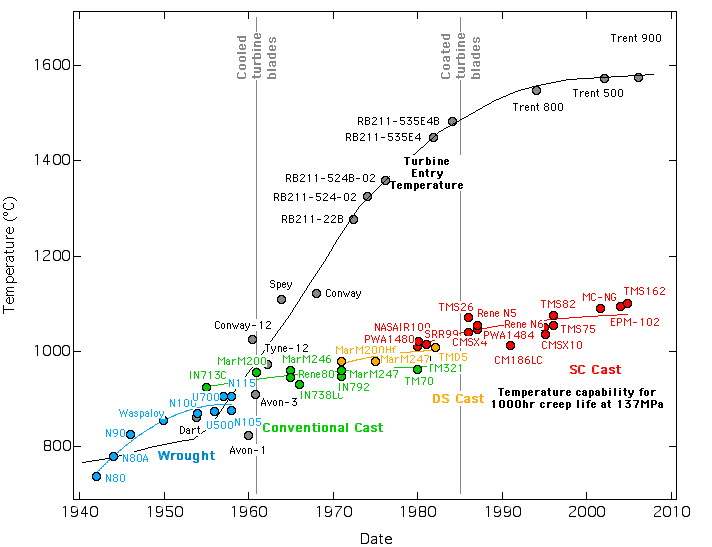
\includegraphics[width=\textwidth]{TET}
\caption{Evolution of the turbine entry temperature (TET) capability of Roll-Royce's civil aeroengines, from 1940 to present.}\label{fig:TET}
\end{center}
\end{figure}
%
\begin{figure}[htbp]
\begin{center}
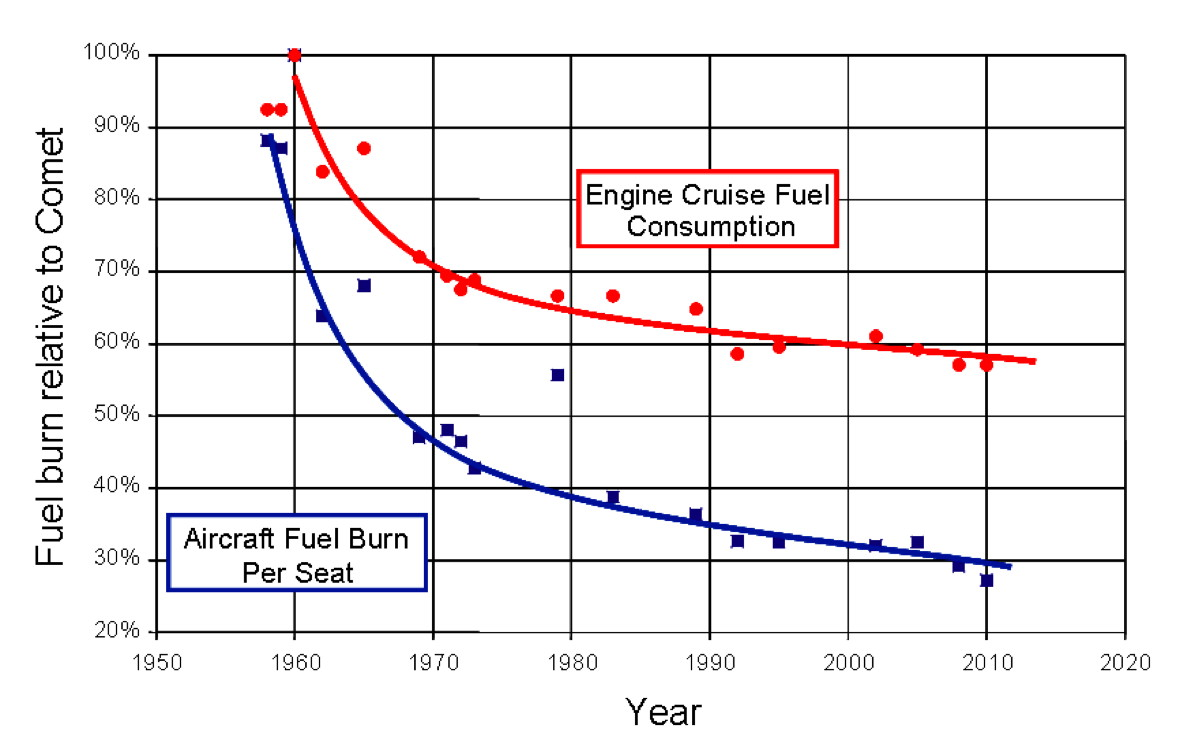
\includegraphics{FuelBurn}
\caption{Fuel burn of Rolls-Royce's civil jet engines, relative to the Comet, from 1960 to present. (Data courtesy of Rolls-Royce masterclass)}\label{fig:FuelBurn}
\end{center}
\end{figure}
%

We want to understand the issues to be faced when designing materials to supercede the commercial nickel-base superalloys used currently. Superalloys have enjoyed unparalleled success for the last 80 years as the high temperature load-bearing material to use ~\cite{reed06}, and there are solid reasons for this. They have a high homologous temperatures, are very resistant to mechanical degradation at high operating temperatures, possess excellent environmental resistance, and are robust, tough and easily machinable ~\cite{betteridge87, sims87}. Knowing how superalloys have evolved, and understanding the difficulties encountered and the successes celebrated thus far by the nickel-base superalloy community provides the starting point for this thesis. An investigation of the most advanced 4$^{th}$ generation superalloys forms the first part of this thesis; the second part is an examination of potential replacement systems and some preliminary results from these materials. 

The incremental approach taken has been to design superalloys with higher temperature capabilities ~\cite{reed06, cumpsty97}.   There have been 3 recognised generations of superalloys defined by alloy composition range. The latest 4$^{th}$ generation superalloys are distinguished by the presences of ruthenium.  Ruthenium was found to suppress topologically close-packed (TCP) phase precipitatation very effectively with little observable detriment to the other desirable properties of superalloys ~\cite{yeh04}.  This permitted the concentration of rhenium, a powerful solid solution strengthener, to be almost doubled without substantial reductions in microstructural stability.  These advanced superalloys with high refractory contents have more highly negative lattice misfits than earlier superalloys, and would directionally coarsen more easily upon the presence of applied stress.  These coarsened precipitates, also known as rafts, are beneficial against high temperature creep.  However, it turns out that this early stage ``rafting" invariably compromises intermediate temperature creep properties, allowing dislocations to cut through them more easily than through unrafted finer cubiodal precipitates ~\cite{hobbs08}.  Understanding the factors that induce early stage rafting, would enable us to determine how to effectively manage them.  

More radical alternative materials to superalloys include two broad classes of materials: intermetallics and ceramics. They offer substantial increases in temperature capability, but have many problems that have not been surmounted as of yet ~\cite{miracle94, kumar94, shah92, sauthoff88, kelly91, kelly96, jackson96, chang91, fleischer94, fleischer85a}. Most notably, their inherent low ductility and fracture toughness at room temperature cause them to have low impact tolerances and to be extremely difficult to process and machine. In this thesis, the compositions that have potential to offer a 100\celsius\ increase in temperature capability over current commercial superalloys will be listed. Systems of compositions that have the potential to realize room temperature fracture toughness and ductility that are higher than current intermetallics and ceramics, while providing the desired increase in temperature capability, will be identified. From literature, eutectic systems with a solid solution toughening phase and a silicide load-bearing phase demonstrate the capacity to fulfill the stated aims. These (Cr,V)$_{solid\ solution}$--(Cr,V)$_3$Si$_{intermetallic}$ eutectics will be characterised to understand their microstructural stability, failure mechanisms, high temperature creep mechanisms and oxidation character.
 
\chapter{Nickel-Base Superalloys}
\section{The Evolution of Nickel-Base Superalloys}

Sims' introduction of the origins of superalloy development in \emph{Superalloys II} ~\cite{sims87} and \emph{The Superalloys} by Reed ~\cite{reed06} both provide excellent overviews on this subject and should be consulted for more detail.  Figure~\ref{fig:evolution} beautifully sums up the evolution of nickel-base superalloys from conception in the 1930s to date, with strengthening phases shown in the top half, and the deleterious phases in the bottom half.
%
\begin{figure}[htbp]
\begin{center}
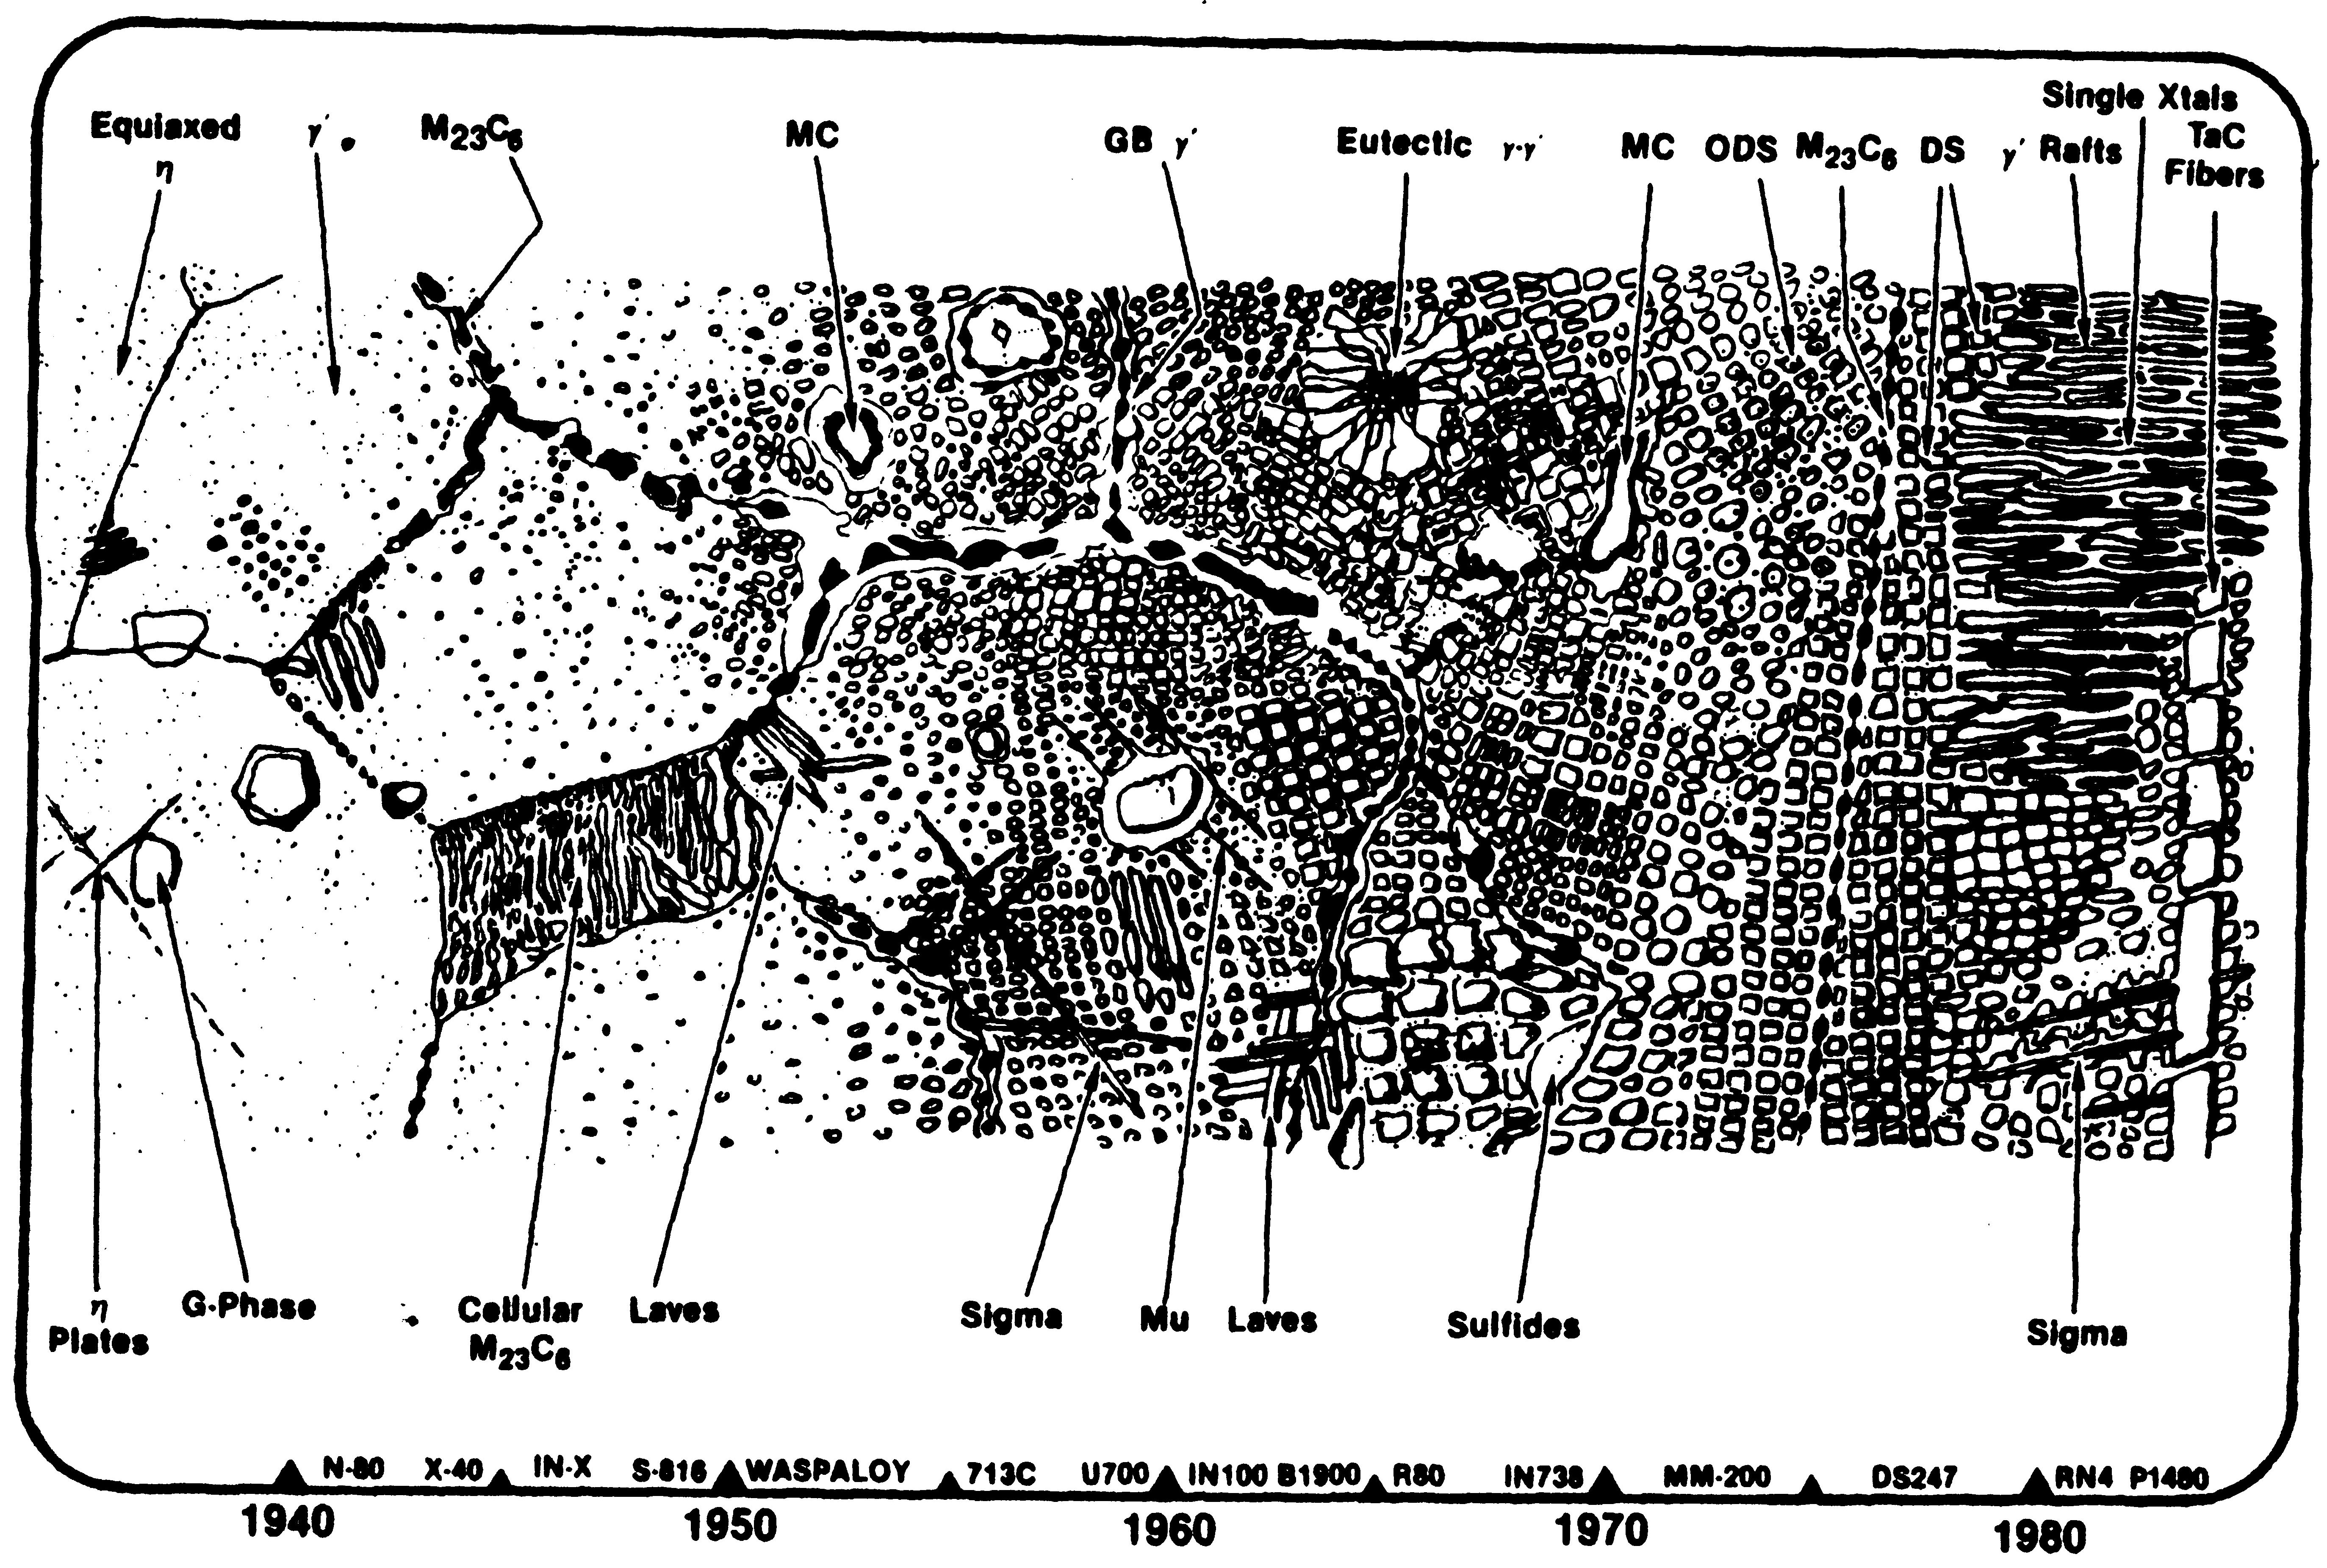
\includegraphics[height=5.5in, angle=90.6]{SuperalloyEvolution}
\caption{Evolution of blade material. Panorama of the development of nickel superalloy microstructure showing both useful and deleterious phases \cite{sims87}.}
\label{fig:evolution}
\end{center}
\end{figure}
%
Superalloys started out as a multi-grained FCC nickel-chromium austenite matrix, with carbides serving as the strengthening phase. This choice of having an FCC matrix is rather fortuitous, as it is now known to be the atomic configuration that can best maintain strength to high homologous temperatures. Aluminium was then found to effectively improve high temperature oxidation resistance, due to the transition of oxide structure from chromia to alumina. Moreover, unbeknownst to the metallurgists, their additions of aluminium also created a small volume fraction of coherent Ni$_3$Al $\gamma'$ precipitates, the sole strengthening phase employed in the most advanced single crystal nickel-base superalloys today. 

With the advent of electron microscopy a decade later, metallurgists were then able to identify carbides and $\gamma'$, and quantify their effects on the high temperature mechanical behaviour alloys. This led to alloys being designed with increasing volume fractions of both phases.  Refractory elements were then found to impart strength to both the solid solution and the precipitates.  Molybdenum was added, followed by tantalum and tungsten. This compromised microstructural stability, and precipitated the formation of embrittling TCP phases. These TCP phases serve as crack nucleation sites, inducing creep cavitation ~\cite{reed99} and causing pre-mature creep failure at high temperatures ~\cite{yeh04}.  As these phases consist mostly of refractory elements, surrounding regions get depleted of their strengthening elements, and this exacerbates localized pre-mature failure. The threshold for solid solution strengthening had been reached.  

Directional solidification was then introduced, allowing for crystal alignment and orientation.  Single crystal superalloys were made possible with the application of grain selectors, which made carbides obsolete, as they were no longer necessary as grain boundary strengtheners.  This widened the heat treatment window and allowed for more complete heat treatment of superalloys.  

In 1986, rhenium was discovered to effectively improve the high temperature mechanical properties of superalloys via solid solution strengthening of the matrix.  Its low diffusivities in nickel at high temperatures were also found to interfere with diffusional creep mechanisms that occur at high temperatures.  Regrettably, its addition induced microstructural instability and inhomogeneity; 2 at.\% resulted in sufficient TCP precipitation to cause premature creep rupture. The alloying ceiling had been reached again.  

Ruthenium was subsequently found to reduce this propensity for TCP formation, by allowing superalloys to tolerate a higher rhenium content. The crystal lattice has to undergo further distortion to accommodate these large refractory atoms, resulting in a more negative lattice misfit.  These superalloys suffer from premature creep failure at intermediate temperatures of 950\celsius, but the reasons for this have not been determined.

Although much of superalloy development has been empirical, the superalloy community is developing advanced modelling techniques to expediate the alloy development process.  Non-linear regression analyses and phase diagram simulations are being used in the prediction of material properties and microstructure. Finite element modelling is used in optimisation of solidification processes.  However, composition, microstructure and processing are very much interdependent. Therefore, it is essential to couple models to incorporate all aspects of alloy design when designing a bespoke product with specific properties.

This is where the superalloys community stands at currently.

\section{Microstructure and Deformation}

In order to understand the consequences of rafting at intermediate temperatures and intermediate stress, it is necessary to detail the superalloy microstructure and its deformation mechanisms during creep in this regime.

\subsection{Dislocations}

The $\gamma$ phase is a nickel-base solid solution with a disordered fcc lattice. The $\gamma'$ intermetallic phase is a Ni$_3$Al fcc superlattice with the L1$_2$ structure. There is a coherent cube-cube orientation  relationship between $\gamma$ and $\gamma'$, and coherent $\gamma'$ precipitates form when lattice misfit is small. These precipitates serve as barriers to dislocation motion, hardening the material ~\cite{copley67}. 

For dislocation motion to proceed, precipitate circumvention or cutting must occur. In commercial blade superalloys, looping of dislocations around precipitates is made difficult by having a high volume fraction of small, discrete particles \cite{reed06, copley67}. This results in narrow matrix channels, which increase the Orowan stress. Dislocation climb is limited by the diffusion rate of the elements at and around the dislocation, and its rate increases with temperature.  During precipitate cutting, an $\frac{a}{2}\left<110\right>$ matrix dislocation moving through an ordered superlattice forms an anti-phase boundary (APB).  The high energy associated with these APBs inhibit dislocation motion through the ordered precipitate.  To minimise this formation energy, the $\frac{a}{2}\left<110\right>$ dislocations typically accomplish precipitate cutting by travelling in pairs or in groups.  The distance between a dislocation pair is dictated by the formation energy of the APB between the dislocations in the precipitate, 
their elastic repulsion energy, the temperature and magnitude of the applied stress. When conditions are unfavourable for either mechanism to proceed, dislocation pile-up occurs at the matrix-precipitate interface, hardening the material.

%There is a driving force from elastic energy of dislocation strain fields for each superdislocation to dissociate into two $\frac{a}{2}\left<110\right>$ dislocations separated by an APB on the $\{111\}$ plane. 

As temperature rises up to 800\celsius, dislocations cross-slip so that the APB fault lies on the $\{001\}$ plane where it has a lower energy. The dislocations become sessile, forming Kear-Wilsdorf locks ~\cite{reed06}. These locks are the cause of the yield stress anomaly, where yield strength increases with temperature. Above 800\celsius, $\gamma'$ softening occurs because the threshold stress for unlocking becomes lower.

MacKay and Ebert hypothesized that the misfit dislocations in the $\gamma$/$\gamma'$  interface are present to relieve the interfacial strains arising from the large negative mismatch~\cite{mackay83}.  These dislocations are similar to those observed in the initial stages of coherency loss of the $\gamma'$ precipitate in long-time aged superalloys, having three-dimensional octagonal networks of $\frac{a}{2}\left<110\right>$ edge dislocations.  Misfit dislocations relax the internal strain energy of a material due to large misfit, therefore decreasing the internal energy of the system. 

Harada and coworkers are of the opinion that dislocations form networks in the $\gamma$ channels that serve as a barrier to precipitate shear, and that these networks hinder the dislocations from entering the vertical $\gamma$ channels.  They hypothesize that superalloys with denser networks would be more resistant to high temperature creep ~\cite{harada06}.

As creep resistance is inversely related to the rate of dislocation motion, an effective means of hindering dislocation motion is precipitate volume fraction optimisation.  The optimal $\gamma'$ volume fraction would minimise the widths of the matrix channels between the precipitates whilst maintaining discreet precipitates.  Dislocations must bow more to enter the matrix channels, which requires higher stress.  Refractory element additions are beneficial as they lower diffusion coefficients and their larger diameters strengthen the solid solution, providing resistance to dislocation motion.


\subsection{Lattice Misfit}

As discussed previously, it is generally desirable for alloys to contain significant quantities of refractory elements to improve creep performance.  Of these elements, only tungsten displays limited partitioning between the matrix and precipitates. Molybdenum and rhenium partition preferentially to the matrix, whilst tantalum partitions to the precipitates \cite{reed04}. In general, however, higher concentrations of refractory elements are typically in the matrix than in the precipitates. The matrix thus has a larger coefficient of thermal expansion than the precipitates. As a consequence, the lattice misfit is typically observed to become more negative upon heating. This has a profound impact on the magnitude of the misfit seen in the alloy at elevated temperature depending upon the composition and hence also the room temperature misfit.

Lattice misfit quantifies the extent of coherency, with larger values signifying higher coherency strains, where the lattice parameter of the precipitate is substantially larger than that of the matrix, or vice-versa.  The lattice misfit is defined by \cite{nabarro96}:
%
\begin{equation}
\delta = \frac{2(a_{\gamma'} - a_\gamma)}{a_{\gamma'} + a_\gamma}
\label{eq:misfit}
\end{equation}
%
The mechanical properties of superalloys have been found to be heavily dependent on $\gamma$/$\gamma'$ interfacial coherency ~\cite{reed06}.  Dislocation movement is impeded by a high lattice misfit due to an increase in elastic strain in the slip plane.  For alloys with positive misfits at room temperature the misfits decrease in magnitude upon heating and may become negative.  In contrast, for an alloy with a negative misfit under ambient conditions, the magnitude of the misfit will typically increase monotonically upon heating.  

With high misfit values, the interfacial energy increases, leading to a more rapid loss of coherency and an increase in the rate of precipitate coarsening.  With the discovery that ruthenium addition allows for increased refractory solubility, refractory element contents have increased, and misfit values have risen accordingly.  It is clear that these higher misfits will not allow coherency to be maintained at the precipitate-matrix interface.  Loss of coherency between the matrix and the precipitate, either by thermal relaxation or through the accumulation of dislocation debris following mechanical deformation, may lead to a reduction in the mechanical properties of the alloy.

\subsection{Creep}

Creep is the plastic deformation at stresses below the flow stress and is dependent on stress, time and temperature ~\cite{nabarro96}.  Reed states that Ni-based single crystal superalloys undergo three stages creep deformation: primary, secondary and tertiary.  He identifies three regimes of creep: primary, tertiary and rafting \cite{reed99}.  

In this report, comments are restricted to the intermediate temperature/intermediate stress tertiary creep regime, with temperature between 850--1000\celsius, and stress between 300--500 \mega\pascal.  In this regime, the three stages of creep are not distinct; instead, there is minimal primary creep, and creep appears to increase logarithmically with time, as the creep strain rate is proportional to the accumulated macroscopic creep strain.

The relevant regime of creep plasticity for the intermediate stress/intermediate temperature creep condition of single crystal nickel-base superalloys is power law creep.  It essentially describes deformation produced by the glide of dislocations in the $\gamma$ phase.  This deformation is limited by dislocation climb around coherent $\gamma'$, which effectively serve as obstacles to prevent plastic flow.  Thermally activated diffusion allow dislocations to climb out of the slip plane, over $\gamma'$ precipitates, and continue to glide along another.  The creep rate is determined by dislocation density and the rate of dislocation movement, and is described by the Orowan equation \cite{nabarro95}:
%
\begin{equation}
\dot{\gamma}  = \rho  b  v  
\end{equation}
%
During high temperature creep, precipitate cutting is difficult due to the lower stress conditions experienced, and this results in dislocations being trapped within the $\gamma$ matrix channels, making dislocation climb around the $\gamma'$ precipitates the dominant mechanism (Figure \ref{fig:LDSX8disloc}). Under intermediate temperature/intermediate stress creep conditions, some precipitate cutting occurs, but precipitate circumvention is dominant. Under low temperature/high stress creep, the stress is experienced by the alloy is high enough to allow precipitate cutting as the principal mechanism for dislocation motion(Figure \ref{fig:LDSX1faults}).
%
\vspace{1cm}
\begin{figure}[H]
\begin{center}
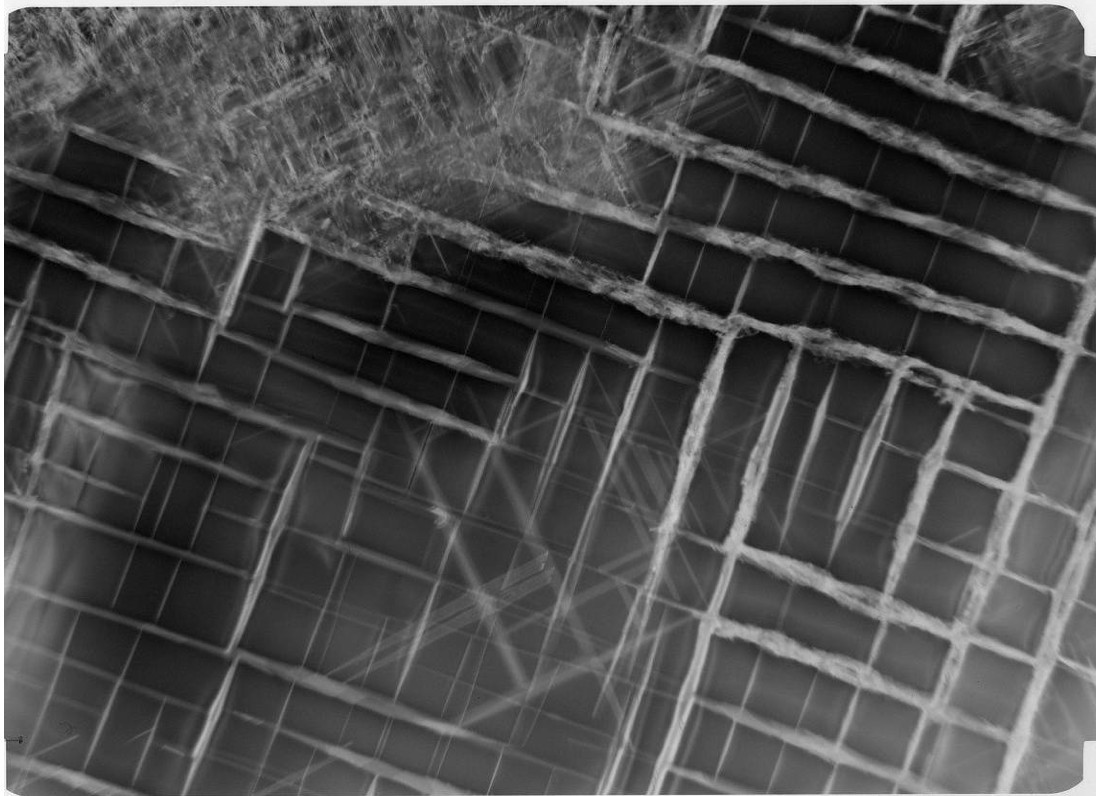
\includegraphics{LDSX8disloc}
\caption{Dislocations located mostly in the $\gamma$ channels of LDSX--8 after heat treatment; very few dislocations have entered the $\gamma'$ precipitates. (courtesy of H.T. Pang)}\label{fig:LDSX8disloc}
\end{center}
\end{figure}
%

\begin{figure}[H]
\begin{center}
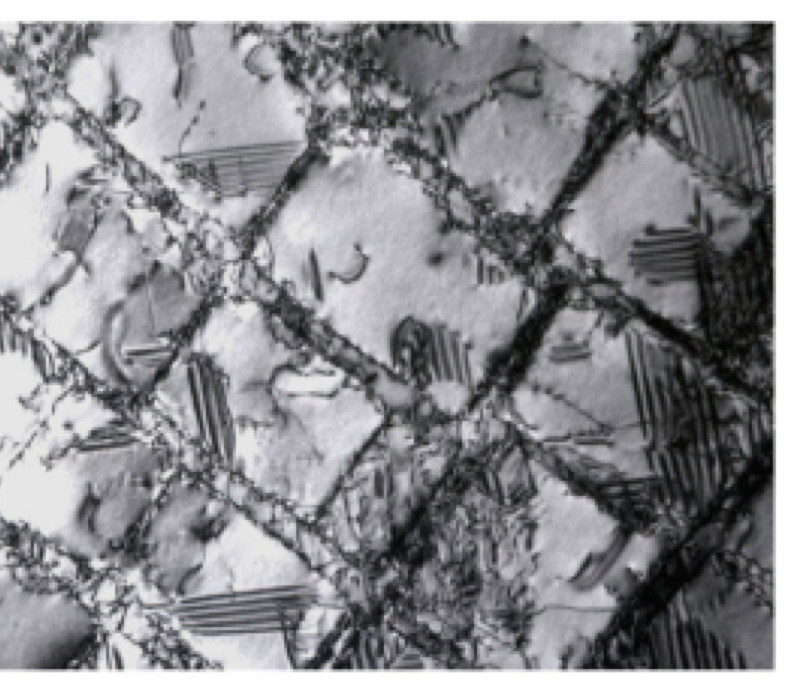
\includegraphics[width=8cm]{LDSX1faults}
\caption{Stacking faults in $\gamma'$ precipitates formed due to dislocation cutting in LDSX--1 after low temperature creep at 750\celsius/800\mega\pascal. (courtesy of L.J. Zhang)}\label{fig:LDSX1faults}
\end{center}
\end{figure}
%
\subsection{Rafting}
When a negatively misfitting alloy is subject to tensile stress at elevated temperatures of above 900\celsius, dislocations form and accumulate in the horizontal channels, relieving the misfit stresses and allowing for the relaxation of coherency stresses on the horizontal $\gamma$/$\gamma'$ interfaces (Figure \ref{fig:CoherencyStress}). This coincides with the cuboidal as-aged $\gamma'$ precipitates coalescing into rafts normal to the tensile loading axis.  This process is known as rafting.  When extensive rafting occurs, the encapsulating $\gamma$ matrix will no longer remain interconnected(Figure \ref{fig:LDSX6rafts}).  
%
\begin{figure}[H]
\begin{center}
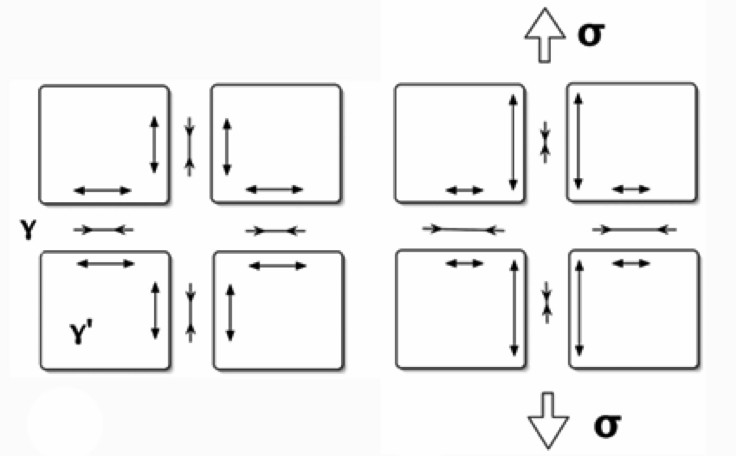
\includegraphics[width=10cm]{CoherencyStress}
\caption{Schematic of coherency stresses arising from an applied tensile stress. (adapted from \cite{reed06})}
\label{fig:CoherencyStress}
\end{center}
\end{figure}
%
\begin{figure}[H]
\begin{center}
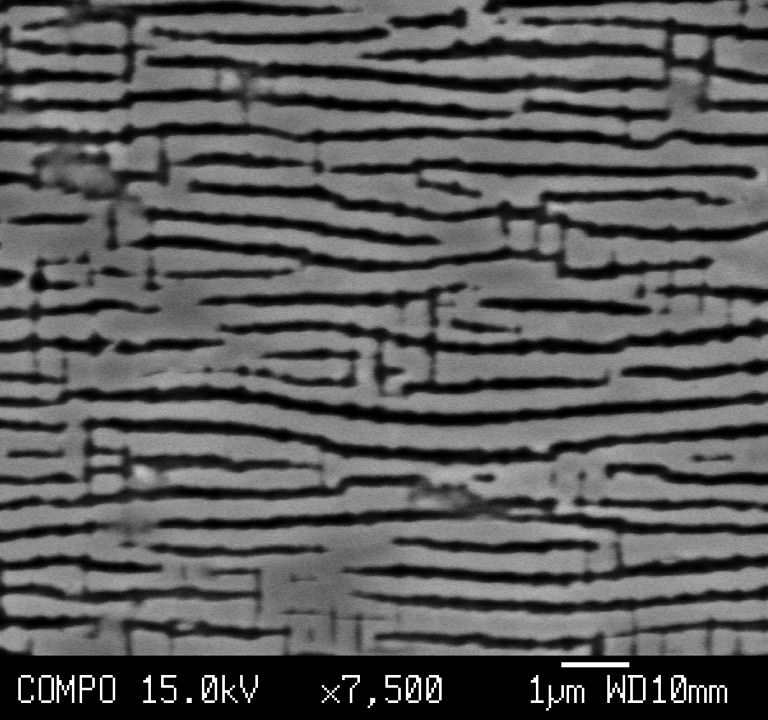
\includegraphics{LDSX6rafts}
\caption{Rafted microstructure of LDSX--6 interrupted after primary creep and subsequent thermal exposure for 500 hours at 950\celsius.}
\label{fig:LDSX6rafts}
\end{center}
\end{figure}
\vspace{-1cm}
%
In the early 1980s, rafting was believed to weaken the alloy's creep properties, due to the increase in interlamellar spacing.  Larger inter-lamellar spacing translates to larger $\gamma$ channels, which do not hinder dislocation motion.  This led to the development of alloys with lower lattice misfit, to obtain minimum coarsening rates with the intention of maximizing creep resistance.  MacKay and Ebert then reported that directional coarsening in single-crystal superalloys with large negative misfit increased creep life by 4 times in the $\left<100\right>$ orientation at 982\celsius\ \cite{mackay83}.  They found rafts were effective barriers to dislocation climb around $\gamma'$.

They observed that once rafts were formed during steady-state creep, the lamellae stabilise and do not undergo further rafting.  A limit had been reached where substantially higher amounts of total strain was required to induce further rafting.  From this, they hypothesised that rafting may be a strain-controlled and time dependent phenomenon.

Factors influencing rafting kinetics are still a subject of controversy.  Reed et al. agree with MacKay's observation that the rafted structure is largely completed at the very early stages of deformation.  Since the rafts are established early, the dislocations, being unable to cut through them under the high temperature/low stress creep conditions, can only move via precipitate circumvention.  The plate-like morphology of these rafts makes circumvention very difficult.  This is probably why superalloys with rafted microstructure perform well during high temperature creep.

Although rafts are beneficial for high temperature creep, they have been found to be detrimental for creep at lower temperatures ~\cite{hobbs08}.  Blade alloys are subject to higher stresses at lower temperatures, this enables dislocations to cut through precipitates.  Since as heat-treated, uncoarsened cuboidal precipitates are finer than the ``rafts", dislocations have a larger energy barrier to surmount for precipitate cutting.  Also, they have a smaller average interparticle spacing, which impedes Orowan dislocation bowing, as the dislocation radius must be very large in order to have sufficient energy to force their way into the smaller $\gamma$ channels.


\section{Background to Experimental Work}
\subsection{The Kinetics of Rafting}

The thermodynamic driving force for rafting depends on the lattice misfit and applied stress.  V\'{e}ron et al. noticed that strain induced during creep seems to be responsible for the rafting phenomenon, and postulated that there is a critical density of plasticity-induced dislocations necessary to induce rafting, and that additional dislocation density above this threshold would have no influence on rafting \cite{veron96}.

A novel method was used by Matan et al. to precisely quantify the kinetics of rafting in a commercial 2$^{nd}$ generation superalloy, CMSX 4, with the aim to evaluate the influence of rafting on creep deformation \cite{matan99}.  Interrupted creep tests at 950\celsius/185 \mega\pascal\ were performed on single crystal heat-treated creep specimens with $\left<100\right>$ orientation parallel to the applied stress, using 20 kN constant load creep testing machines.  The tests were interrupted  at 150, 280, 500, 695, 1060 and 1170 hours.  The tested specimens were sectioned axial to the direction of applied stress, and micrographs were taken and stereologically characterised.  Degree of rafting was seen to increase with the length of creep testing.

The threshold strain for rafting to proceed in the absence of applied stress was determined.  The threshold strain was found to be 0.10$\pm$0.03\%.  When a specimen was strained beyond the threshold strain, it continues to raft during subsequent annealing in the absence of applied stress.  If accumulated strain is below the threshold strain, subsequent annealing does not promote further raftingMatan et al. postulated that the thermodynamic driving force and the kinetics of rafting in the plastic regime would be correlated to the lattice misfit. This will be investigated by looking at three alloys in the LDSX series with representative low, medium and high lattice misfits.

\subsection{Effect of Misfit on Creep Properties}

The LDSX series comprises of eight 4$^{th}$ generation alloys that has been developed at the Rolls-Royce University Technology Centre are currently undergoing evaluation.  The nominal compositions and predicted misfit values by JMatPro$^{\copyright}$ are shown in Table~\ref{tab:LDSXcomps}.

Alloys with representative low, intermediate and high misfits, LDSX--1, 6 and 8, have been chosen for this study, as seen in Figure \ref{fig:MisfitJMatPro}.  LDSX--1 is the least alloyed, with the lowest content of Mo, Re and W, and consequently, possesses the lowest misfit.  LDSX--8 has the highest refractory element content, and the highest predicted misfit.  A commerical second generation superalloy, CMSX-4, will be used as reference.
%
\begin{table}[htdp]
\begin{center}
\begin{tabular}{lccccccccccc}
\hline\hline
Alloy 	&     Ni    &  Al   &  Co  &   Cr &   Mo     &Ti     & Ta    & W     &Re &    Ru    & Hf\\\hline
LDSX-1  &   Bal.&    6.0&    3.0&     3.0&     2.5&    0.25&    6.5&    2.9&    6.2&     3.5&     0.1\\LDSX-2    & Bal.&    6.0&    8.0&     3.0&     5.0&    0.25&    6.5&    2.9&    6.2&     3.5&     0.1\\LDSX-3     &Bal.&    6.0&    3.0&     3.0&     5.0&    0.25&    6.5&    4.8&    6.2&     3.5&     0.1\\LDSX-4 &    Bal.&    6.0&    8.0&     3.0&     2.5&    0.25&    6.5&    4.8&    6.2&     3.5&     0.1\\LDSX-5 &    Bal.&    6.0&    8.0&     3.0&     2.5&    0.25&    6.5&    2.9&    6.2&     5.0&     0.1\\LDSX-6  &   Bal.&    6.0&    3.0&     3.0&     2.5&    0.25&    6.5&    4.8&    6.2&     5.0&     0.1\\LDSX-7  &   Bal.&    6.0&    3.0&     3.0&     5.0&    0.25&    6.5&    2.9&    6.2&     5.0&     0.1\\LDSX-8  &   Bal.&    6.0&    8.0&     3.0&     5.0&    0.25&    6.5&    4.8&    6.2&     5.0&     0.1\\
\hline\hline
\end{tabular}
\end{center}
\caption{Nominal compositions of LDSX--1 to 8.}\label{tab:LDSXcomps}
\end{table}
%
\begin{figure}[H]
\begin{center}
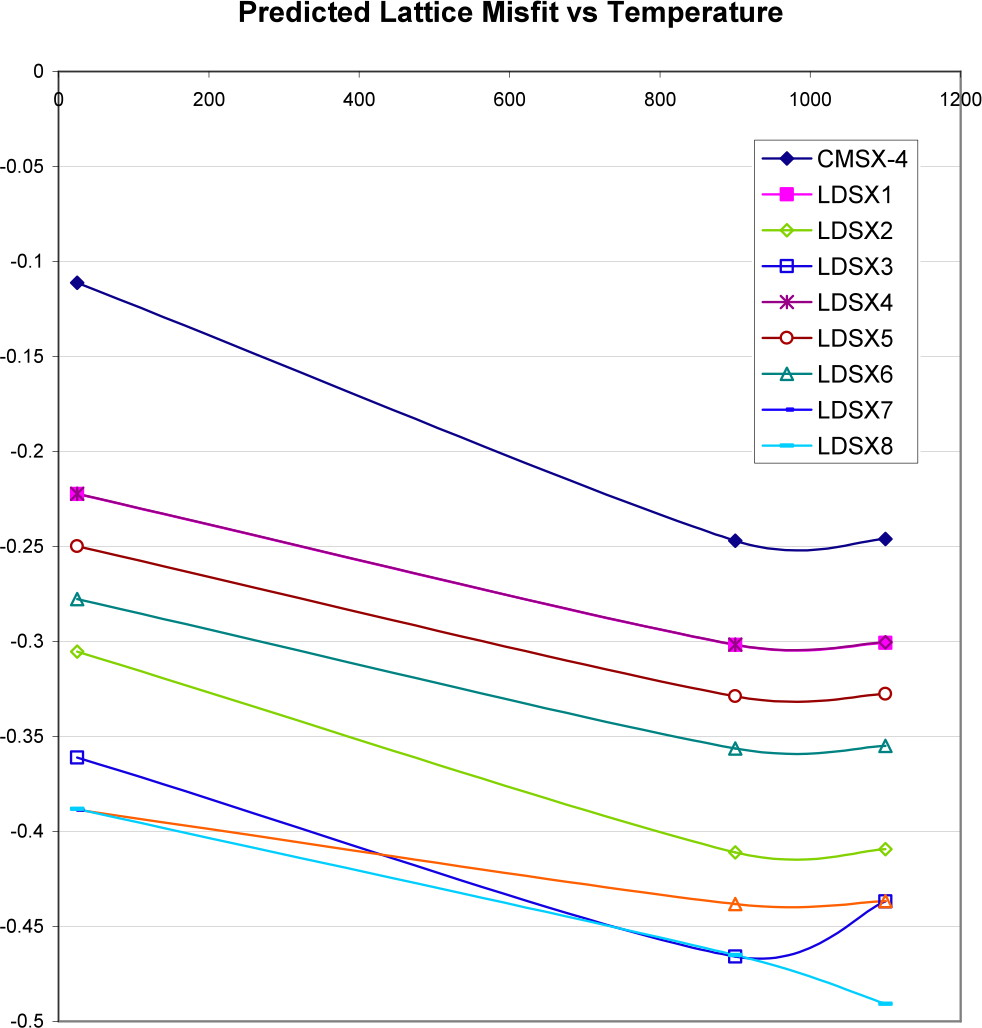
\includegraphics{MisfitJMatPro}
\caption{Predicted misfit as a function of temperature for LDSX--1, 6 and 8.}
\label{fig:MisfitJMatPro}
\end{center}
\end{figure}
%
The more heavily alloyed LDSX--6 with higher lattice misfit took a longer time than LDSX--1 to reach the same elongation.  The most heavily alloyed LDSX--8, suffered from premature rupture, and had half the rupture life of LDSX--1.  Additionally, LDSX--8 had no visible incubation period, and a mere two hours of primary creep.  This premature failure can be due to several factors.  It has a highly negative misfit, and is noted to be prone to TCP precipitation. 




\section{Experimental Work}

Bars of alloys designated LDSX--1, 6 and 8 were directionally-solidified to produce single crystals with $\left<001\right>$ orientation at the Precision Casting Facility (PCF) in Derby, England.  The bars were solution treated to eliminate casting segregation: LDSX--1 at 1340\celsius\ for 10 hours, LDSX--6 at 1340\celsius\ for 10 hours, and LDSX--8 at 1360\celsius\ for 15 hours.  They were then primary aged at 1150\celsius\ for 4 hours and secondary aged at 870\celsius\ for 16 hours to eliminate secondary $\gamma'$. 

Tensile creep specimens were machined from LDSX--1, 6 and 8.  Their $\theta$/$\rho$ angles, showing their relative orientation to the loading axis, were 4.2/36.4, 13.0/18.7 and 3.0/28.8, respectively.  They were crept at 950\celsius/375\mega\pascal\ and the tests were stopped when the onset of secondary creep was observable.  Sections were cut out from the gauge lengths of these interrupted creep specimens.  They were then subject to thermal exposure at 950\celsius, the temperature that the specimens were crept at, for a subsequent 10, 50, 100, 200, 500 or 3000 hours.  Microstructural examination was performed with a JEOL 6340F FEGSEM, where micrographs representative areas were taken to quantify microstructural stability and the extent of rafting in these alloys. 

Misfit measurements are difficult to obtain for nickel-base superalloys by diffraction using conventional laboratory X-ray sources.  The $\left<001\right>$ $\gamma$ peaks are invisible in fully ordered structures.  The $\left<001\right>$ $\gamma'$ peak is visible but it is very weak and requires a long data collection time when using a typical X-ray source available at universities.  This leads to instrumental line broadening, a source of error.  Also, the $\left<002\right>$ peaks of $\gamma$ and $\gamma'$ overlap and are very difficult to separate.  In order to split these peaks accurately, the $\left<001\right>$ $\gamma'$ peak position, which indicates its lattice parameter, can be used to ``fix" the position of the $\gamma'$ peak, which allows us to determine the peak position $\gamma$ through curve deconstruction. X-rays produced at a synchrotron are of higher intensity, and much shorter acquisition times would be required.  Measurements of the lattice parameters of the $\gamma$ matrix phases and $\gamma'$ precipitate phases of the alloys were performed on the BM28 beamline at the European Synchrotron Radiation Facility (ESRF) in Grenoble, France.  Monochromation of the X-rays was achieved by diffraction from a double-crystal Si $\{111\}$ monochromator to give an incident energy of 11.9 \kilo\electronvolt\ with a wavelength of 1.0418 \angstrom.  The beam was 0.5$\times$0.5 \milli\meter\ at full width at half maximum (FWHM), with a resolution of 1.7$\times$10$^{-4}$, and was focused on the sample surface using a torroidal mirror.

Transverse sections of the bars with $\left<001\right>$ nominally vertical were mounted on a goniometer head attached to an 11-axis Huber diffractometer.  This permitted the sample to be translated in x, y and z within the diffractometer and orientated in four circles ($\phi$ , $\chi$ , $\omega$, 2$\theta$).To establish the orientation of the sample, the 2$\theta$ angle was set at a value consistent with the expected lattice parameter of the material and $\phi$ varied until a strong diffraction signal was detected.  For samples with significant off-axis orientations, scans in $\phi$ were performed as chi was increased to locate the $\left(001\right)$ pole.  Once established, 2$\theta$ was increased to an angle consistent with diffraction from a $\left(111\right)$ pole and the sample reoriented accordingly before scanning in $\phi$ to indentify the pole.  Knowledge of the orientations of these two poles permitted automatic reorientation of the sample to other poles for detailed measurement.

The $\left(001\right)$ \& $\left(003\right)$ superlattice reflections and $\left(002\right)$ \& $\left(004\right)$ fundamental reflections were scanned in \emph{h} \& \emph{k} to generate two-dimensional reciprocal space maps.  It was considered necessary to characterise the superlattice reflections so that the lattice parameter of the $\gamma'$ could be uniquely determined and enable unambiguous identification of the contribution of the $\gamma'$ to the overlapping fundamental reflections.  The low atomic scattering contrast between the atoms occupying the face and corner sites in the $\gamma'$ necessitated long acquisition times for the superlattice reflections.  Three dimensional reciprocal space maps showing intensity in $h$ and $k$ were generated by stepping $h$ and $k$ in increments of 0.0025 \angstrom\ at 1 second per point.  The measured misfit values were compared with values predicted by JMatPro$^{\copyright}$.The interfacial dislocation networks form during creep as a result of $\frac{a}{2}\left<110\right>\{111\}$ creep dislocations being held up at the $\gamma$/$\gamma'$ interface. Misfit can also be calculated by measuring the average dislocation spacing along the $\left<110\right>$ direction in these networks through TEM observation.

\section{Results and Discussion}

\subsection{Microstructural Stability and Degree of Rafting}

LDSX--1, 6 and 8 all display the onset of rafting prior to the presence of applied load (Figure \ref{fig:LDSXAsAged}). When subject to interrupted creep at an intermediate temperature of 950\celsius, LDSX--1 and 6 raft perpendicular to the direction of applied stress (Figure \ref{fig:LDSXInterrupted}).  The more highly misfitting LDSX--6 rafts quicker and more extensively than LDSX--1.  On the other hand, LDSX--8, predicted by JMatPro$^{\copyright}$ to have a highly negative misfit, undergoes substantial precipitate coarsening in all 3 $\left<001\right>$ directions prior to stress being applied.  This has been termed the labyrinth structure.  This is unusual; superalloys generally raft only after sufficient plastic deformation has occurred ~\cite{reed99}.

After further thermal exposure, LDSX--1 continues rafting, with marked precipitate coalescence after 200 hours (Figure \ref{fig:LDSXInterrupted_200}).  LDSX--1 shows a stable phase structure over the timescale of these tests; TCP precipitation was unusual, even after 500 additional hours at 950\celsius (Figure \ref{fig:LDSXInterrupted_500}).  This shows that creep rupture in LDSX--1 was not due to phase instability.
%
\begin{figure}[hp]
\begin{center}
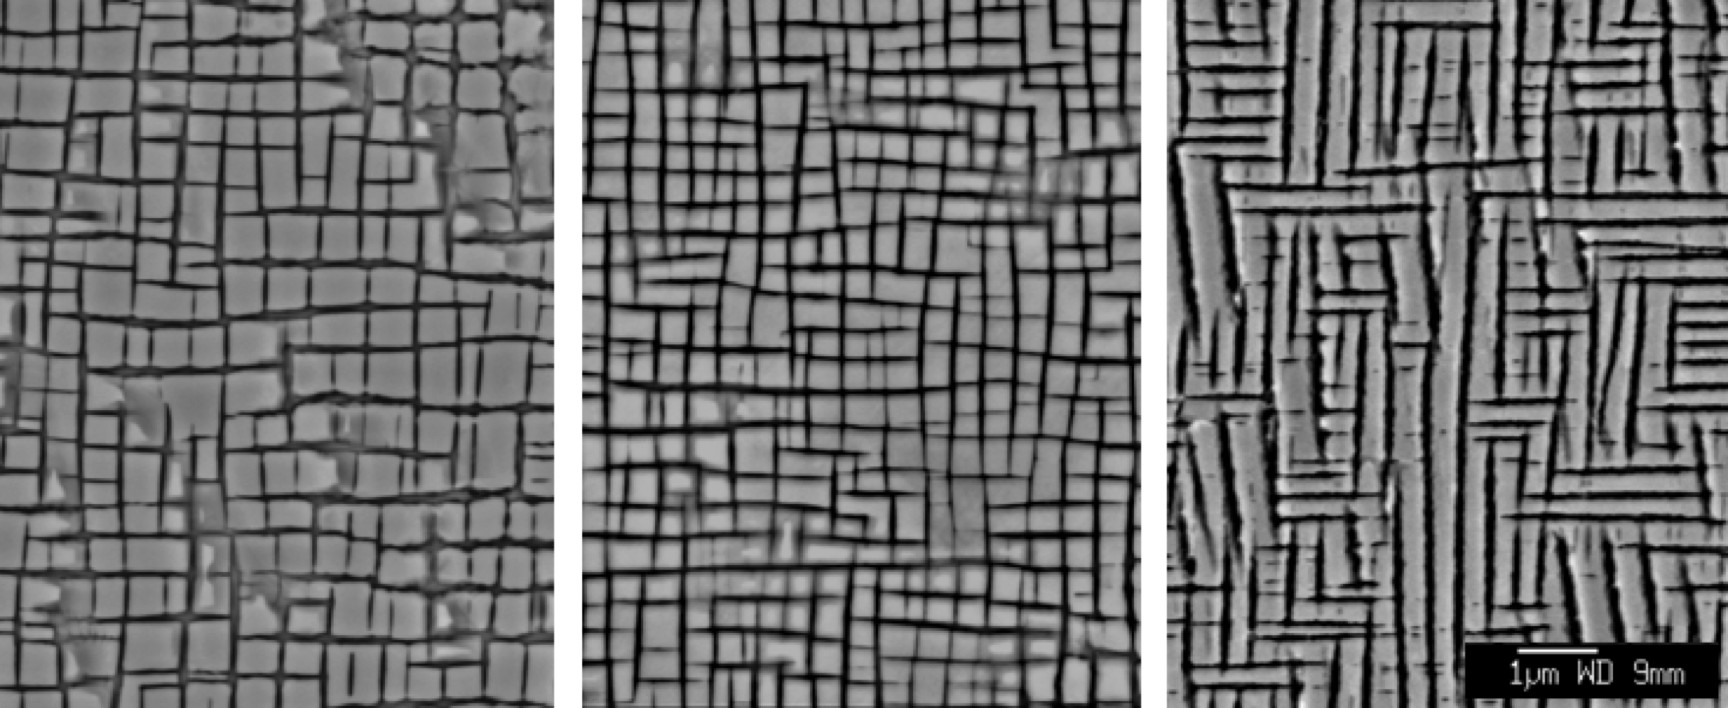
\includegraphics{LDSXAsAged}
\caption{LDSX--1, 6 and 8: as aged}\label{fig:LDSXAsAged}
\end{center}
\end{figure} 
%
\begin{figure}[hp]
\begin{center}
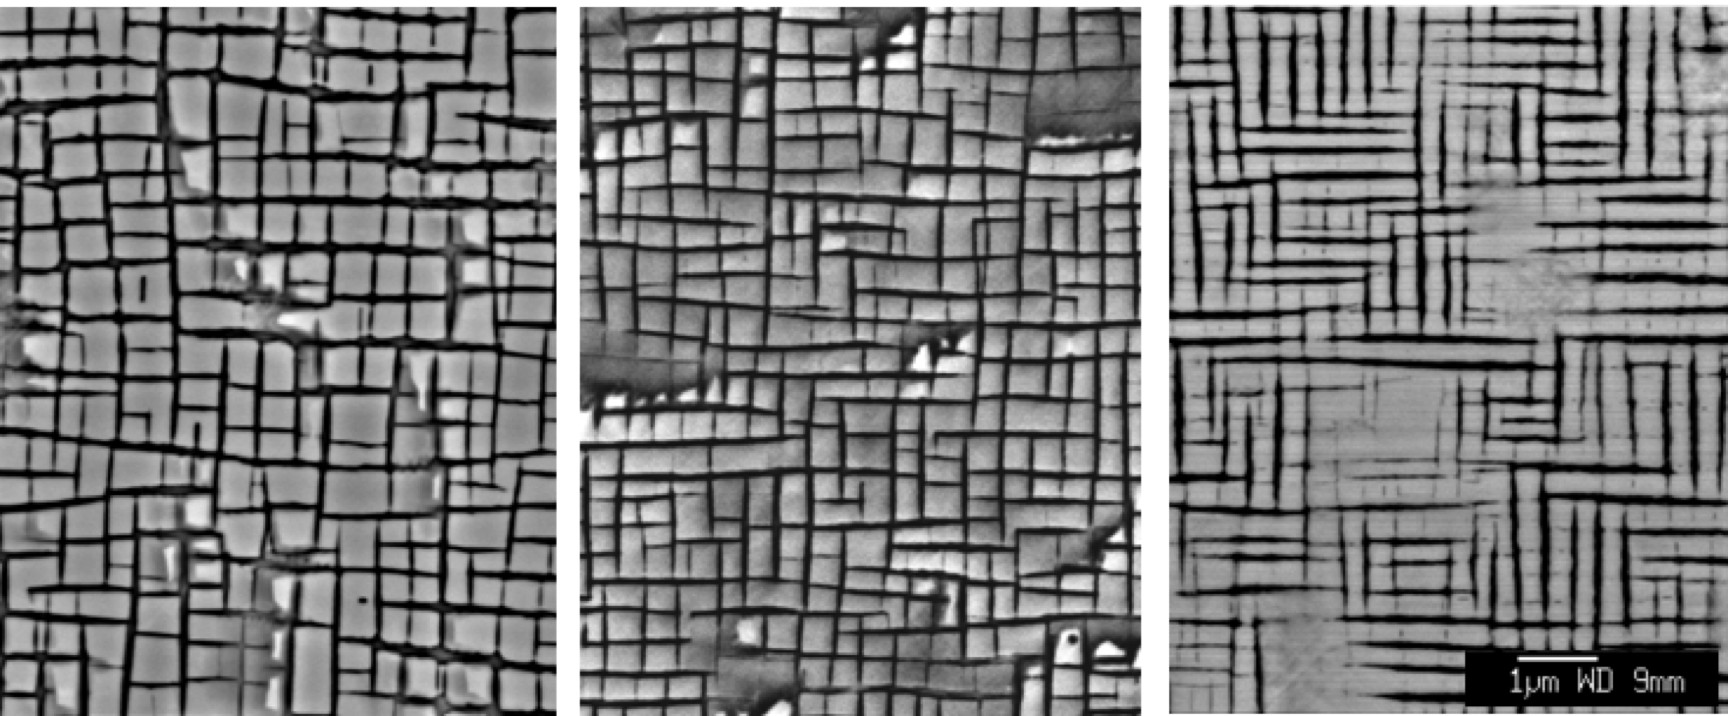
\includegraphics{LDSXInterrupted}
\caption{LDSX--1, 6 and 8: as interrupted crept }\label{fig:LDSXInterrupted}
\end{center}
\end{figure} 
%
\begin{figure}[hp]
\begin{center}
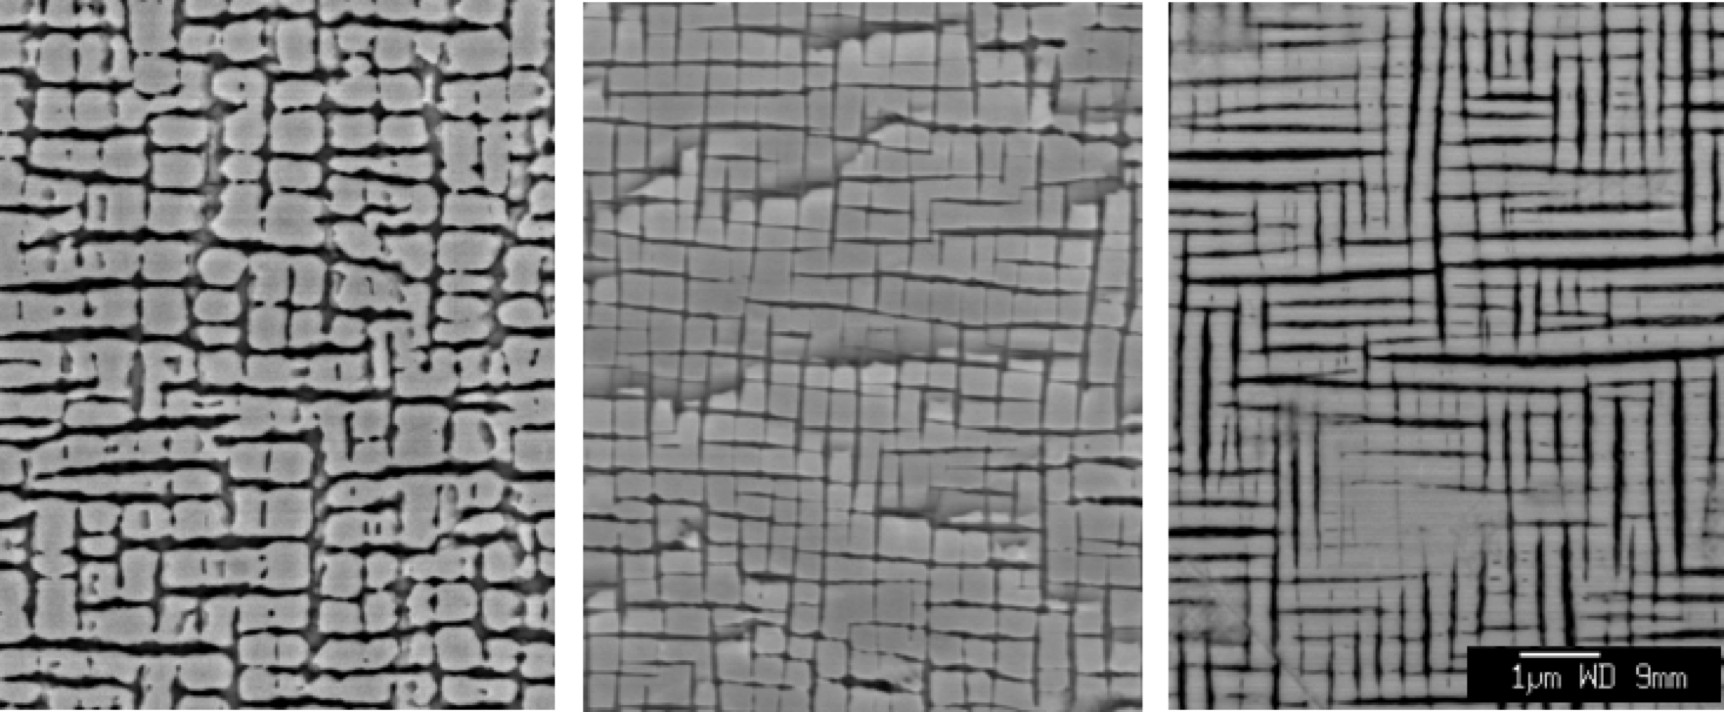
\includegraphics{LDSXInterrupted_10}
\caption{LDSX--1, 6 and 8: as interrupted crept + 10 hours at 950\celsius}\label{fig:LDSXInterrupted_10}
\end{center}
\end{figure} 
%
\begin{figure}[hp]
\begin{center}
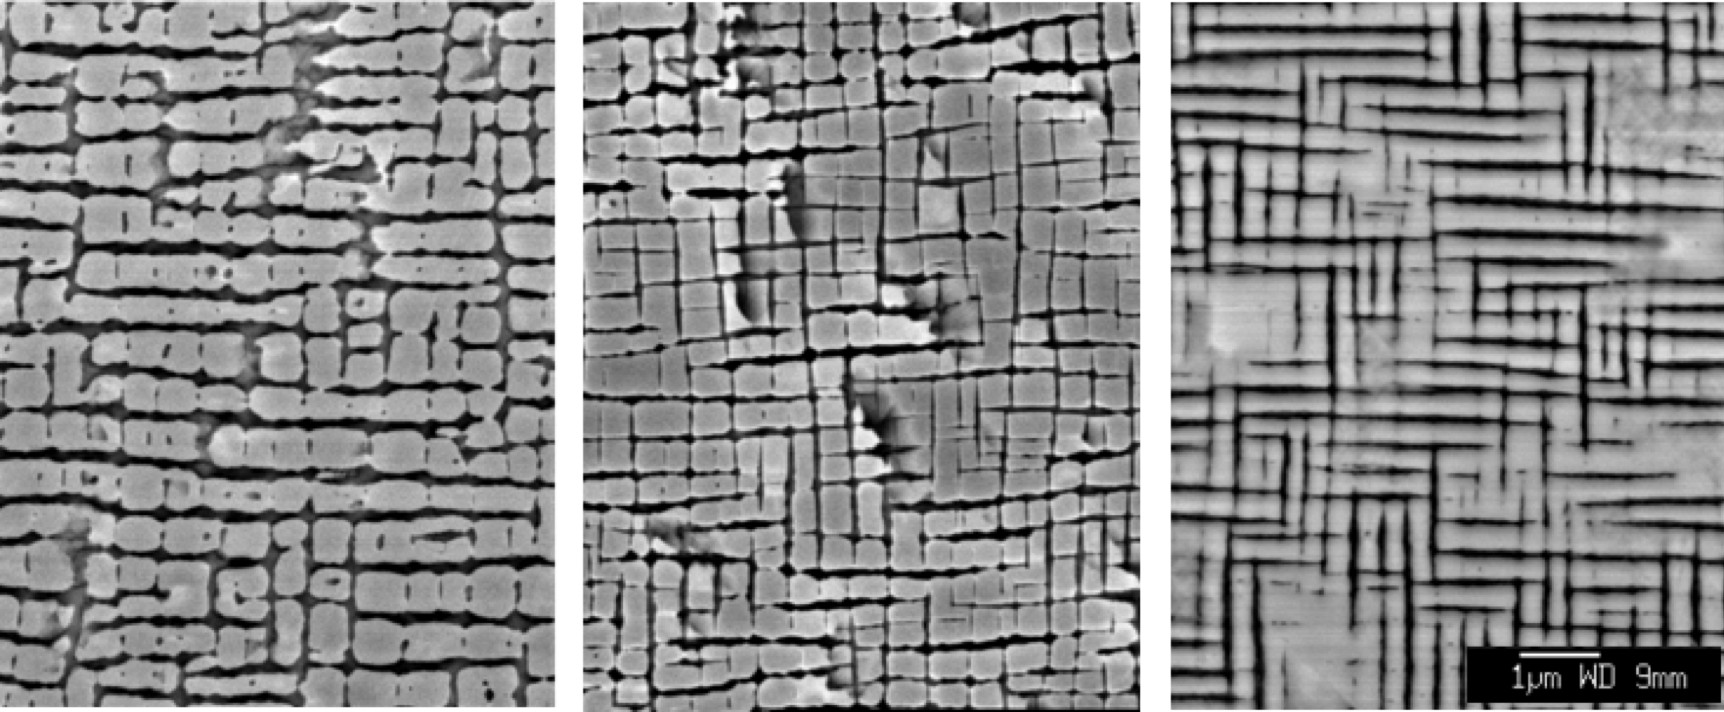
\includegraphics{LDSXInterrupted_50}
\caption{LDSX--1, 6 and 8: as interrupted crept + 50 hours at 950\celsius}\label{fig:LDSXInterrupted_50}
\end{center}
\end{figure} 
%
\begin{figure}[hp]
\begin{center}
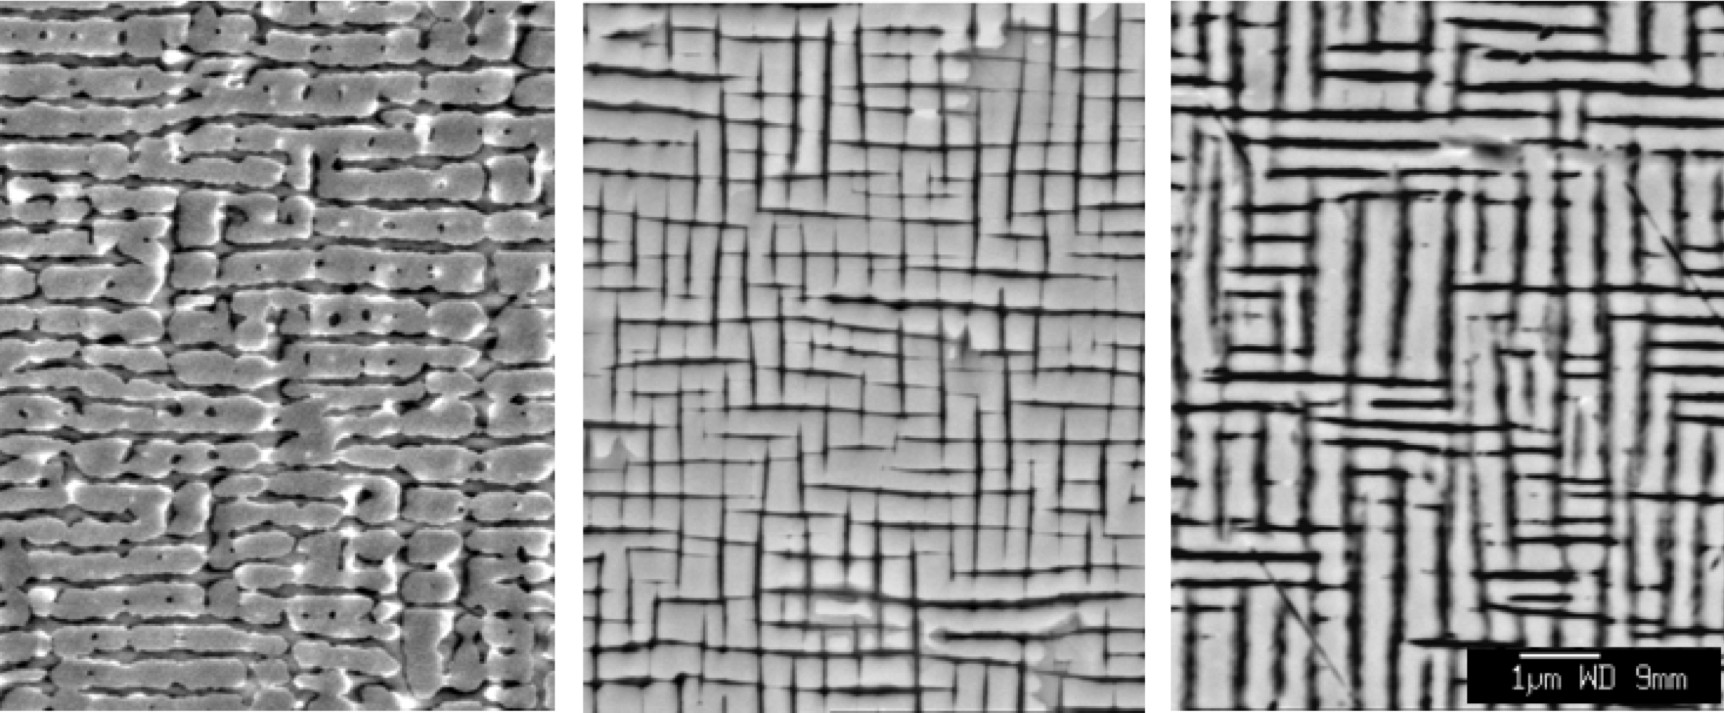
\includegraphics{LDSXInterrupted_200}
\caption{LDSX--1, 6 and 8: as interrupted crept + 200 hours at 950\celsius. }\label{fig:LDSXInterrupted_200}
\end{center}
\end{figure} 
%
\begin{figure}[hp]
\begin{center}
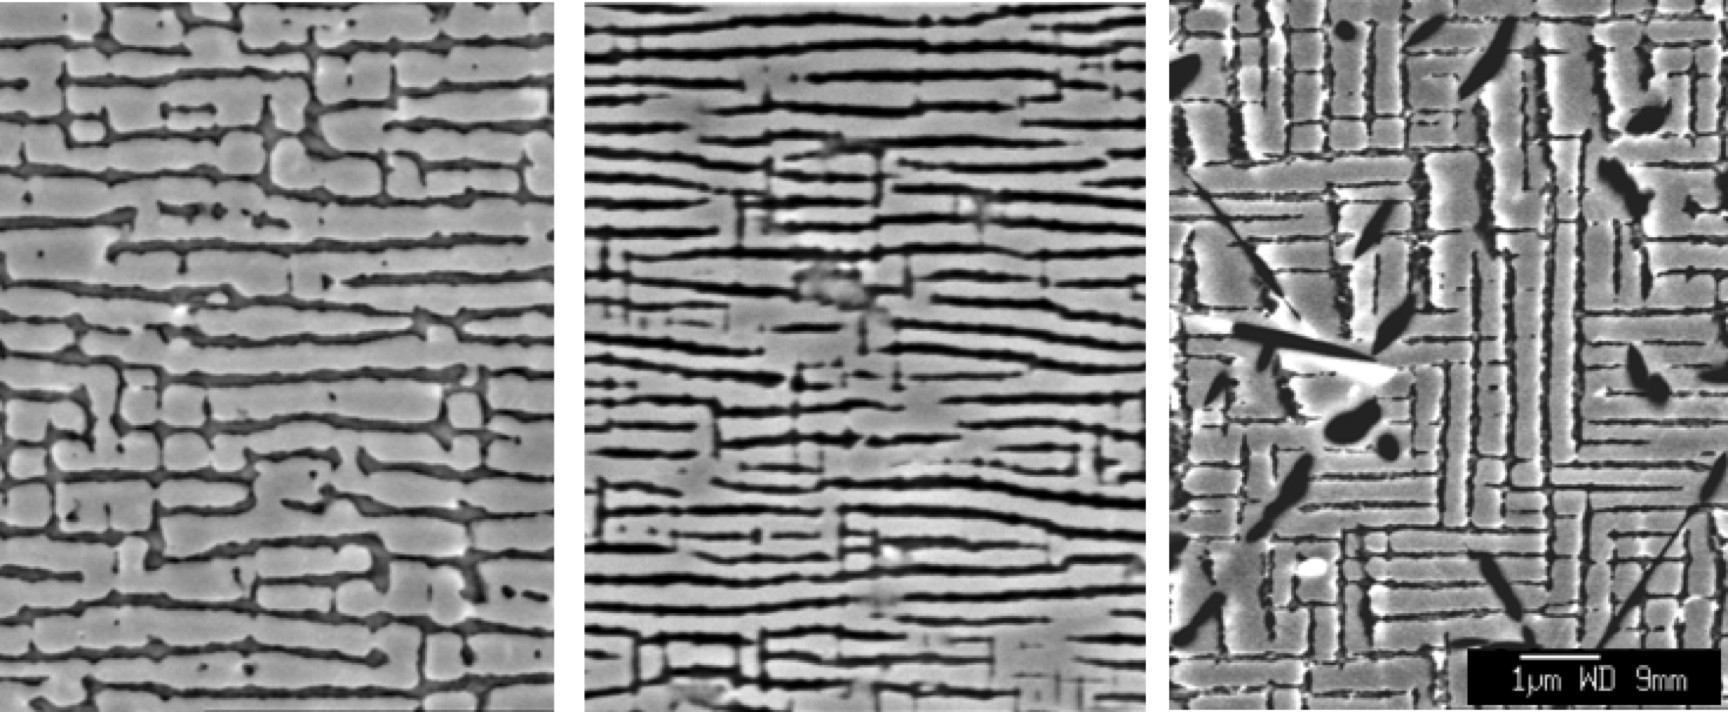
\includegraphics{LDSXInterrupted_500}
\caption{LDSX--1, 6 and 8: as interrupted crept + 500 hours at 950\celsius.}\label{fig:LDSXInterrupted_500}
\end{center}
\end{figure}
%
In LDSX--6, some TCP precipitation was seen in the dendrite core regions after 200 additional hours at 950\celsius\ (Figure \ref{fig:LDSXInterrupted_200}).  The volume fraction of precipitates is not substantial enough to adversely affect creep properties.  This is consistent with LDSX--6 having the longest creep life.  

Dislocations were observed in the $\gamma$ channels of the as heat treated LDSX--8 in TEM (Figure \ref{fig:LDSX8disloc}). They were unobservable in the as heat treated SEM sample (Figure \ref{fig:LDSXAsAged}) because the specimen was sectioned at an angle to the $\{001\}$ plane, which did not allow large portions of $\gamma$ channels to be observed.  The presence of dislocations prior to application of stress is quite unusual.  Dislocation networks became noticeable in the dendritic regions of the interrupted creep specimen after a subsequent thermal exposure of 10 hours (Figure \ref{fig:LDSXInterrupted_10}).  Their density increased with thermal exposure length.  Their presence indicates that the $\gamma$/$\gamma'$ interfaces have lost coherency by forming these stress-relieving networks (Figure \ref{fig:LDSX8disloc}).  

LDSX--8 is microstructurally unstable.  Rampant precipitation was observed after 200 hours at 950\celsius, and most dendritic regions contained substantial TCP precipitates (Figure \ref{fig:LDSXInterrupted_200}).  This extensive TCP precipitation is detrimental to creep properties, as it depletes the surrounding microstructure of strengthening elements.  The removal of these elements reduces the alloy's lattice misfit, but rafting was not halted nor reversed, as can be seen in the specimen that had been exposed for 500 hours at 950\celsius\ (Figure \ref{fig:LDSXInterrupted_500}). 

It is difficult to isolate the influence that lattice misfit has on creep from the influence of the extent of TCP precipitatation; these two factors have a very strong correlation, as can be seen in LDSX--8.  Lattice misfit becomes more negative upon the addition of select refractory elements; this also increases rafting and promotes TCP precipitation. 

The premature failure of LDSX--8 in creep will have to be attributed to both its highly rafted labyrinth structure and the extensive precipitation of TCPs.  Figure \ref{fig:LDSXCreep} shows time to \% strain for the three alloys.  LDSX--8 showed the poorest properties and took 60 hours to reach 1\% elongation.  The specimen with the closest thermal history available had been interrupted after 2 hours of primary creep at 950\celsius, and subjected to a further 50-hour thermal exposure (Figure \ref{fig:LDSXInterrupted_50}).  This specimen has a large population of dislocation networks.  The TCP precipitates visible are sparsely scattered, and are unlikely to adversely affect the mechanical properties of the alloy substantially.  From this, it can be said that the poorer performance of LDSX--8, as seen from its shorter time to 1\% elongation at 950\celsius\ when compared to LDSX--6, is exclusively due to its labyrinth structure.  The creep rupture time for LDSX--8 is even worse; it is half that of LDSX--6.  At this stage, TCP precipitation probably has a stronger negative influence than the labyrinth structure.

MacKay and Ebert state that the wider $\gamma$ channels resulting from rafting would adversely affect creep rates at 950\celsius.  Comparing the times to 0.5\% strain of the three alloys, strain rates increase with increasing misfit.  The alloy with the least propensity to raft, LDSX--1, has the longest time to 1\% strain.  This is consistent with the opinion of MacKay and Ebert ~\cite{mackay83}.  When we look at the times to 2\% strain, the strain rate of LDSX--6 between 0.5\% and 2\% is markedly slower than LDSX--1, as the time to 2\% strain is equal in both alloys.  These results suggest that wider $\gamma$ channels impact creep only to a small extent, and this impact is limited to initial creep strain.  These channels may allow the dislocations to travel a larger distance with ease, but once the dislocations encounter a $\gamma'$ precipitate, they are captured at the $\gamma$/$\gamma'$ interface, and cannot travel further.  In fact, we suggest that the $\gamma'$ precipitates in LDSX--6 may be stronger than those in LDSX--1 due to the higher content of refractory elements present, and they pose a larger resistance to precipitate cutting by dislocations, thereby improving creep resistance and allowing for LDSX--6 to display a longer time to creep rupture than LDSX--1.

An increase of misfit improves creep performance, but a misfit larger than the optimum level is is detrimental to creep. We do not see an adverse effect due to the extent of rafting; LDSX--6 rafts to a greater extent than LDSX--1, but has better creep properties.  A negative effect is only seen when the labyrinth structure is present. 

The diffusion coefficient of $\gamma$ is one magnitude higher than that of $\gamma'$, and allows the refractory elements to cluster together with more ease in the former, nucleating TCP precipitates ~\cite{reed06}.  This is why TCP precipitates are mostly located in the wider $\gamma$ channels where there are substantial dislocation networks.  These networks serve as fast diffusion paths for the slow-diffusing refractory atoms to agglomerate into TCP precipitates.  It is interesting to note that although LDSX--6 is less stable than LDSX--1 with respect to TCP precipitation, it is also stronger with the slowest creep at all strains above 2\% (Figure \ref{fig:LDSXCreep}).   

These results suggest there is an upper limit on the useful magnitude of the negative misfit and thus the concentration of refractory elements used to strengthen the $\gamma$-matrix at intermediate temperatures.  At lower temperatures, misfit appears beneficial for creep at 750\celsius.  But as the temperature rises, high misfit can cause spontaneous rafting to give a labyrinth structure.  This appears to be detrimental for creep at 950\celsius\ even before substantial TCP precipitation is observed.  This can be tested by producing a microstructure in LDSX--8 without the labyrinth rafting through a suitable heat treatment.
%
\begin{figure}[H]
\begin{center}
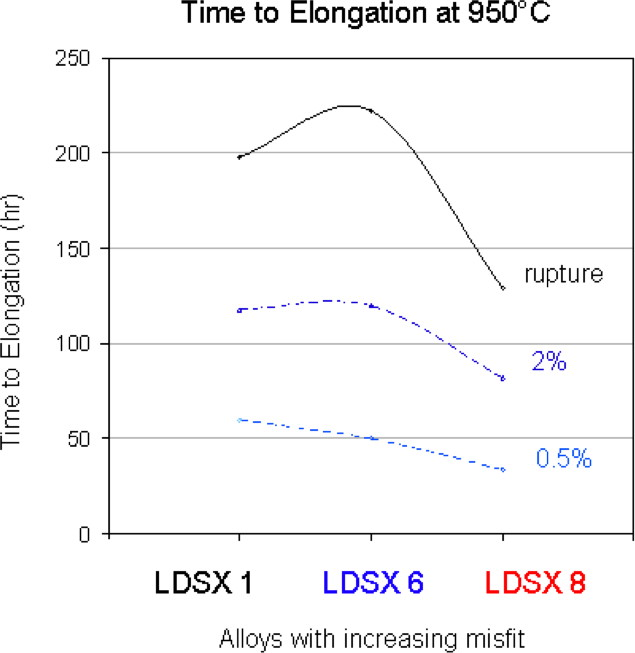
\includegraphics[width=9cm]{LDSXCreep}
\caption{Time to \% percent elongation of LDSX--1, 6 and 8 at 950\celsius/ 375\mega\pascal.}
\label{fig:LDSXCreep}
\end{center}
\end{figure}
%
\begin{figure}[H]
\begin{center}
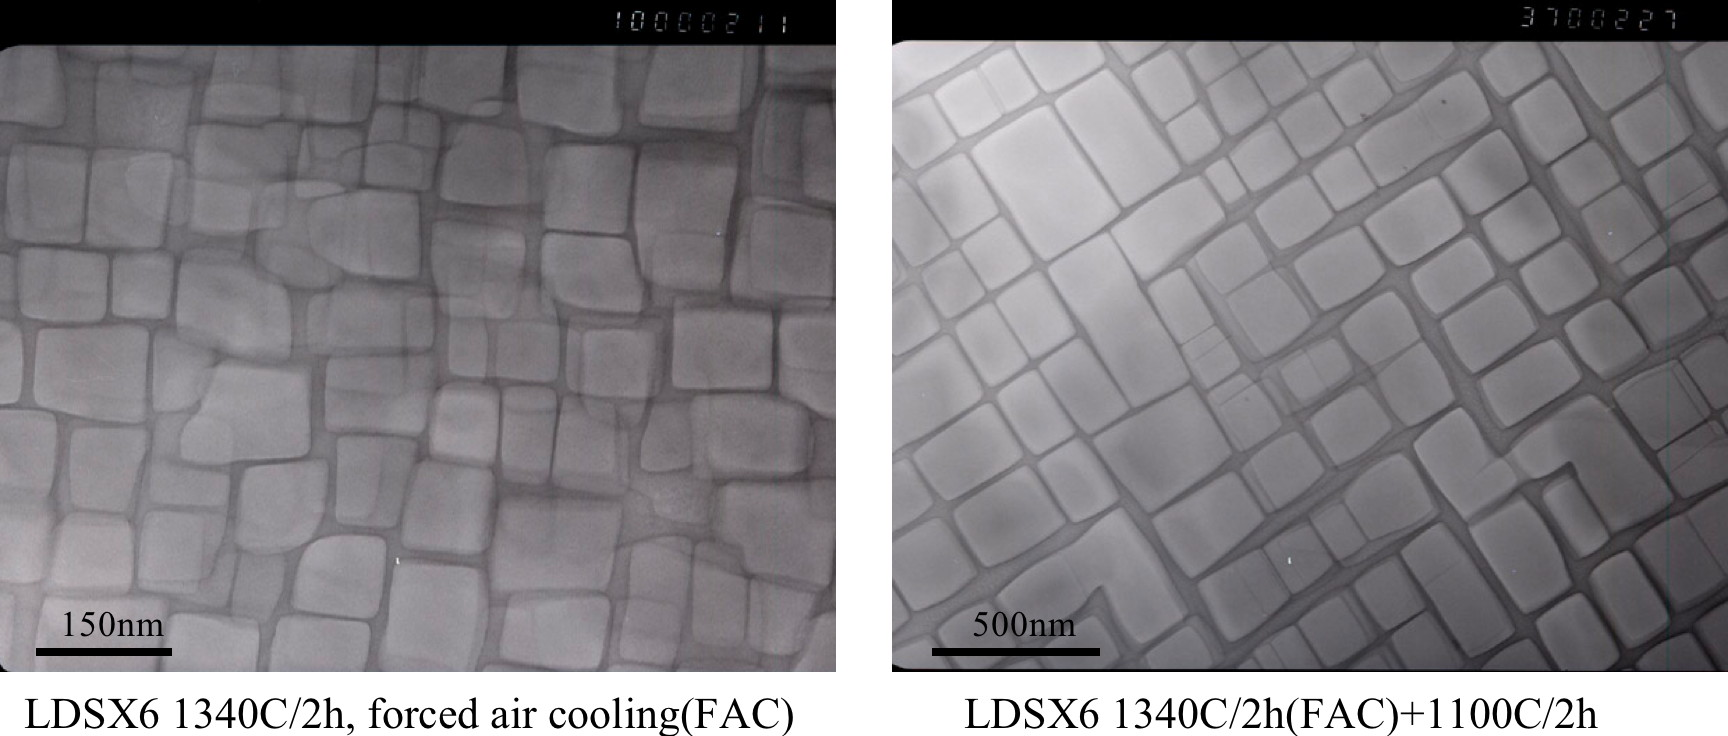
\includegraphics{LDSX6HT}
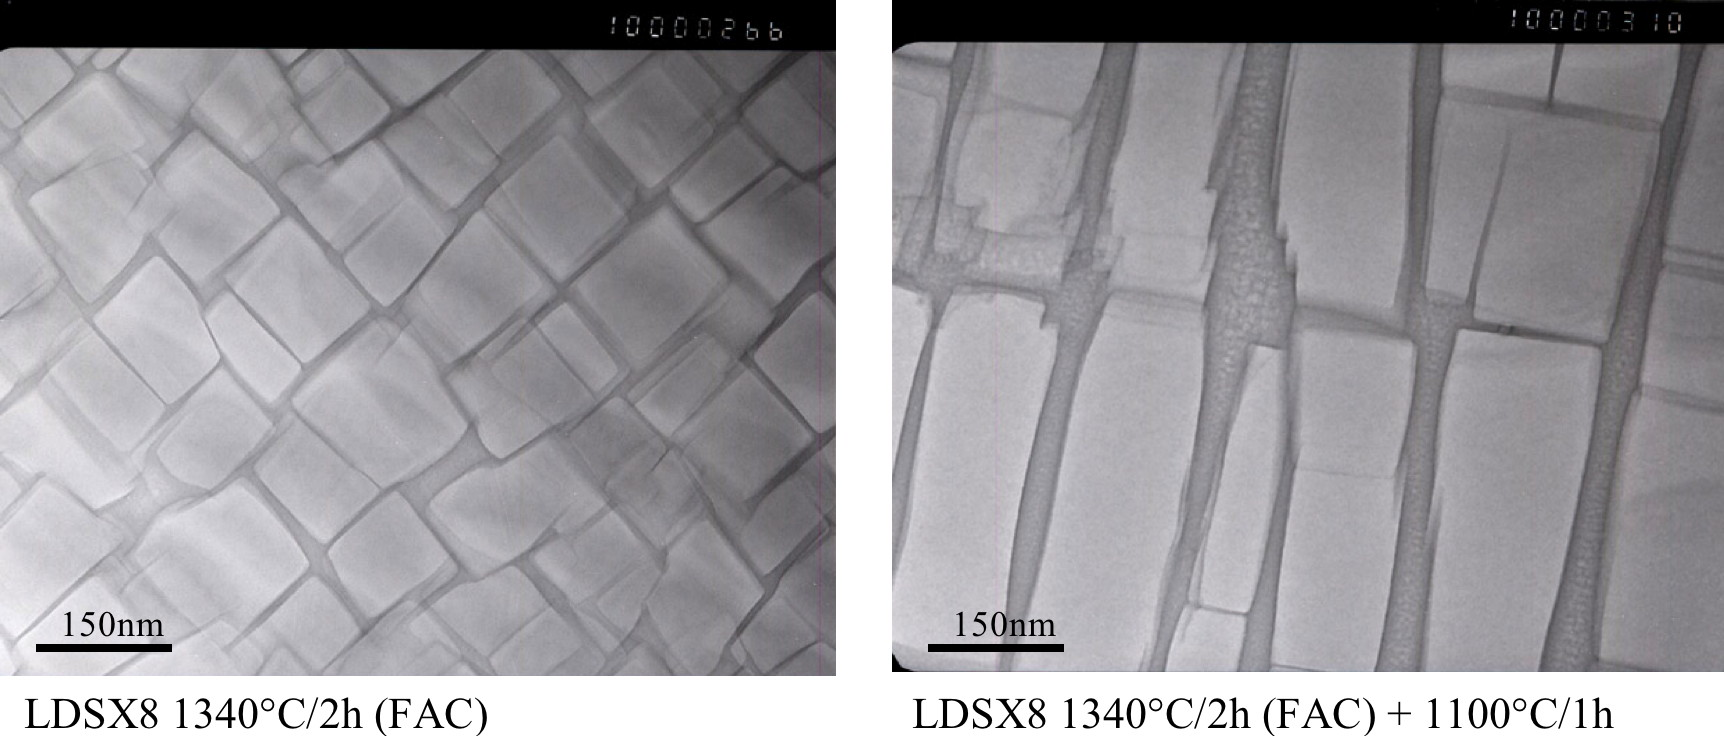
\includegraphics{LDSX8HT}
\caption{TEM micrographs of LDSX--6 and 8 after various heat treatments.}
\label{fig:LDSXHT}
\end{center}
\end{figure}
\vspace{-8mm}
%
Typically, a nickel-base superalloy that has been homogenised has to undergo an ageing treatment to achieve a uniform distribution of cubiodal $\gamma'$ precipitates.  This ageing treatment is performed at 1100\celsius\ for a few hours, as this is the temperature required for the diffusion step of the application of low-cost platinum-aluminised bond coats used as protection against high temperature corrosion and oxidation ~\cite{reed06}.  As seen in Figure \ref{fig:LDSXHT}, the $\gamma'$ precipitates of LDSX--6, become more cuboidal and orderly after 2 hours at 1100\celsius .  

Figure \ref{fig:LDSXHT} shows the microstructures of LDSX--6 and 8 after an additional solution heat treat of 2 hours at 1340\celsius\ followed by an air quench.  This process produces a finer $\gamma'$ size than conventional cool in a commercial furnace.  In the case of the highly misfitting LDSX--8, precipitate coalescence occurs after 1 hour at 1100\celsius, which is disadvantageous for low and intermediate temperature creep.  The as-homogenised LDSX--8 specimen that underwent an additional 1340\celsius\ for 2 hours seems to have a sufficiently optimised microstructure; the $\gamma'$ precipitates are cubiodal.  If the labyrinth structure seen in the as-aged specimen is detrimental to the creep properties of LDSX--8, the as-homogenised specimen should out-perform the as-aged specimen in creep.  A creep test at 950\celsius/ 375\mega\pascal\ will be conducted on this as-homogenised sample and compared to the creep results of the as-aged specimen.  This will indicate the extent of which labyrinth rafting is causing the poor creep properties.

\subsection{Measurement of Lattice Misfit}

Two-dimensional and three-dimensional plots (Figure \ref{fig:3Dplot}) of intensity in reciprocal space were obtained at the ESRF. There are two $\gamma$ peaks due to the different lattice parameters of the constrained $\gamma$ in the vertical channels and the unconstrained $\gamma$ in the horizontal channels. The peaks from $\gamma'$ and the constrained $\gamma$ were fitted, and theirlattice parameters were used to calculate the lattice misfits using Equation \eqref{eq:misfit}. The calculated misfit values (Table \ref{tab:misfitesrf}) are higher than the predicted values (Table \ref{tab:misfitjmatpro}). 
 
\begin{figure}[H]
\begin{center}
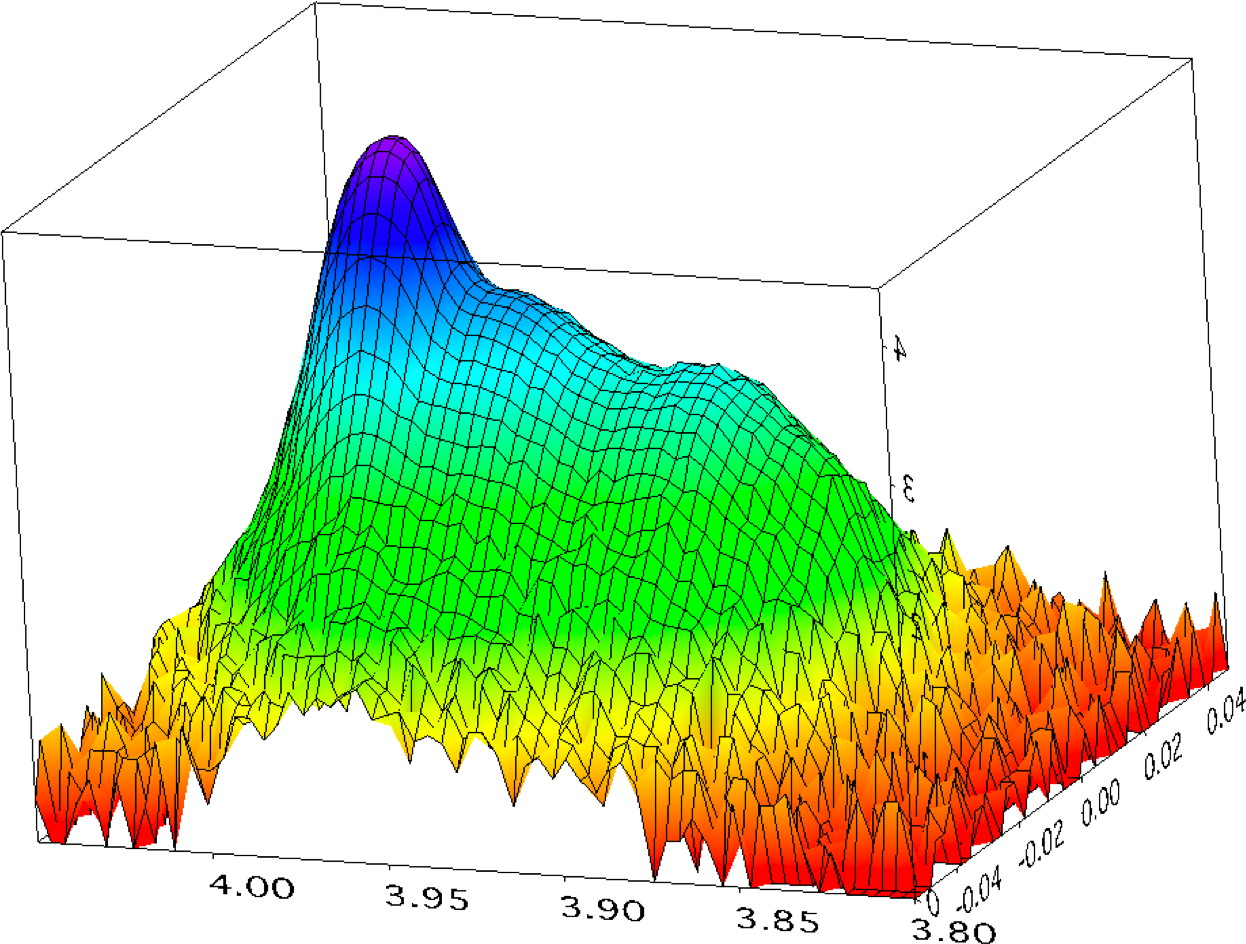
\includegraphics{3Dplot}
\caption{3D plot of LDSX--8 as HT}\label{fig:3Dplot}
\end{center}
\end{figure}

 
%
\begin{table}[H]
\begin{center}
\begin{tabular}{l c c c c} 
\hline
\hline
Alloy & 	Phase    &	Reciprocal lattice distance   &Lattice distance &	Misfit 	\\
\hline
\multirow{2}{*}{LDSX--1}&	$\gamma$ &	3.96944					&3.62029	&	\multirow{2}{*}	{-0.77\%}	\\
	 &	$\gamma'$&	4.00004					&3.59259	&				\\
\multirow{2}{*}{LDSX--6}&	$\gamma$ &	3.96443					&3.62486	&	\multirow{2}{*}	{-0.85\%}	\\
 	 &	$\gamma'$&	3.99827					&3.59418	&				\\
\multirow{2}{*}{LDSX--8}&	$\gamma$ &	3.96783					&3.62176	&	\multirow{2}{*}	{-0.78\%}	\\
	 &	$\gamma'$&	3.99896					&3.59356	&				\\
\hline
\hline
\end{tabular}
\end{center}
\caption{Lattice misfit values of LDSX--1, 6 and 8, obtained at the ESRF. }
\label{tab:misfitesrf}
\end{table}


\begin{table}[H]
\begin{center}
\begin{tabular}{l c c } 
\hline
\hline
Alloy&	Temp (\celsius) &	Misfit (\%)\\
\hline
&	25	&-0.11\\
CMSX-4	&900	&-0.25\\
	&1100&-0.25\\
	\hline
&	25	&-0.22\\
LDSX--1	&900	&-0.30\\
	&1100&	-0.30\\
	\hline
&	25	&-0.31\\
LDSX--2	&900	&-0.41\\
	&1100&	-0.41\\
	\hline
&	25&	-0.36\\
LDSX--3	&900&	-0.47\\
	&1100&	-0.44\\
	\hline
&	25	&-0.22\\
LDSX--4	&900	&-0.30\\
	&1100&	-0.30\\\hline
&	25&	-0.25\\
LDSX--5	&900	&-0.33\\
	&1100&	-0.33\\
	\hline
&	25&	-0.28\\
LDSX--6	&900	&-0.36\\
	&1100&	-0.35\\
	\hline
&	25&	-0.39\\
LDSX--7	&900	&-0.44\\
	&1100&	-0.44\\
	\hline
&	25&	-0.39\\
LDSX--8	&	900&	-0.47\\
	&	1100&	-0.49\\
\hline
\hline
\end{tabular}
\end{center}
\caption{Lattice misfit values of LDSX--1, 6 and 8, predicted by JMatPro$^{\copyright}$. }
\label{tab:misfitjmatpro}
\end{table}
% INPUT SILICIDE HALF
\chapter{Exploration of Alternative Systems}

There are three broad classes of material that have been explored as aero-engine blade material: metal alloys, ceramics and intermetallics.  Most metal alloys suitable for high-temperature application have been explored thoroughly over the last fifty years.  They suffer from decreases in strength at low homologous temperatures, have high densities and/or costs (W, Pt), and possess poor oxidation resistances (Mo, Nb, W).  Consequently, metal alloys have lower operating capabilities than intermetallics and ceramics, and are unsuitable for higher temperature operation.  

This leaves us with two categories of systems that have suitable candidates for high-temperature applications.  The first category are systems based on ceramics.  The options include: monolithic ceramics and ceramic matrix composites (CMCs).  The second category of systems are based on intermetallic phases.  The options are: monolithic or multi-phase intermetallics, metal-intermetallic materials. 

The academic community has identified various ceramic systems that have potential as successors to nickel-base superalloys.  Ceramics have very high melting points; some ceramics have the ability to retain strength at temperatures beyond 2000\celsius\ (Figure \ref{fig:CeramicsIntermetallics}).  However, the greatest hurdle faced by both monolithic ceramics and CMCs is their intrinsic lack of room temperature toughness ~\cite{evans80}.  Due to the nature of their atomic bonds, it is unlikely that this can be surmounted.  For this reason, we will not be exploring ceramics further in this work.

Several monolithic and multi-phase intermetallic systems are seen to offer a compromise between the room temperature robustness of superalloys and the high-temperature capabilities of ceramics ~\cite{nathal92, balsone01}.  Their room temperature toughnesses, however, are insufficient.  Several rather creative approaches that have been tried include:

\begin{enumerate}

\item ductile ligament toughening through utilising a softer second phase ~\cite{flinn89}
\item transformation toughening (which has been successfully employed in TRIP steels) ~\cite{evans86}
\item crack-deflection toughening ~\cite{strum94}
\item micro-crack toughening ~\cite{kumar91}
\end{enumerate}

Many stoichiometric intermetallics suitable for high-temperature applications do not have the fracture-toughness required for manufacture and processing ~\cite{kumar91}.  Intermetallic systems will hence not be considered in this work. 

Through this process of elimination, the thesis will focus on the options available in the realm of metal-intermetallic composites.
%
\begin{figure}[H]
\begin{center}
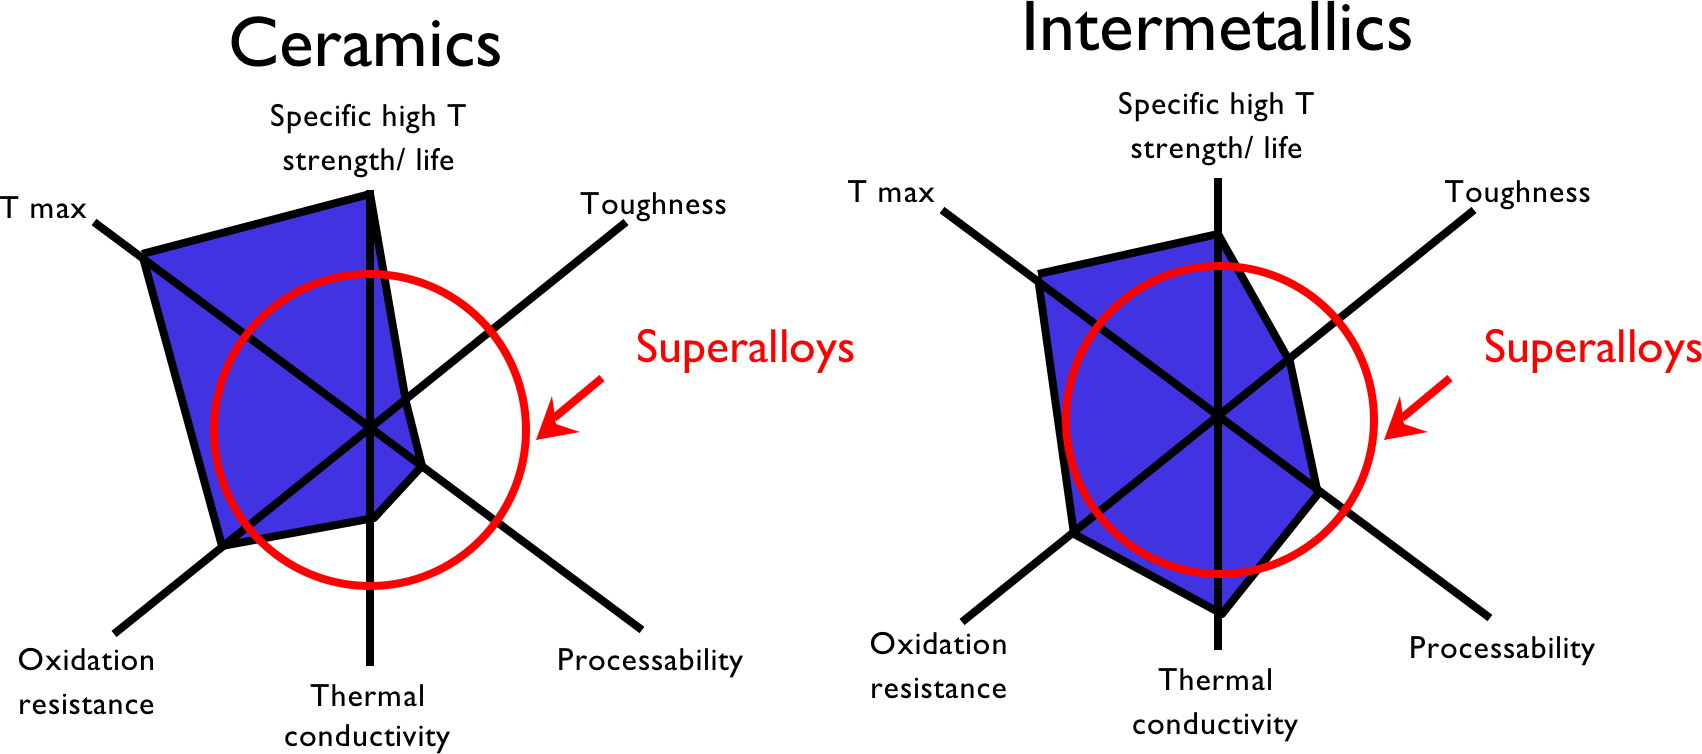
\includegraphics[width=\textwidth]{CeramicsIntermetallics}
\caption{Properties of ceramics and intermetallics compared to superalloys (adapted from ~\cite{nathal92}.) }\label{fig:CeramicsIntermetallics}
\end{center}
\end{figure}
%

Resistance to oxidation during exposure between room and operating temperatures is a neccessity for blade materials.  This prevents catastrophic failure through runaway oxidation occurring.  Whilst coatings may be used to protect the alloy, if the coating should fail in service, the alloy must possess sufficient oxidation resistance to survive between service intervals.  The three oxides through which oxygen has the lowest permeability are those of aluminium, chromium and silicon (Figure \ref{fig:oxidepermeability}).  To base our alloy system on one of these elements would be a sound start.

%
\begin{figure}[H]
\begin{center}
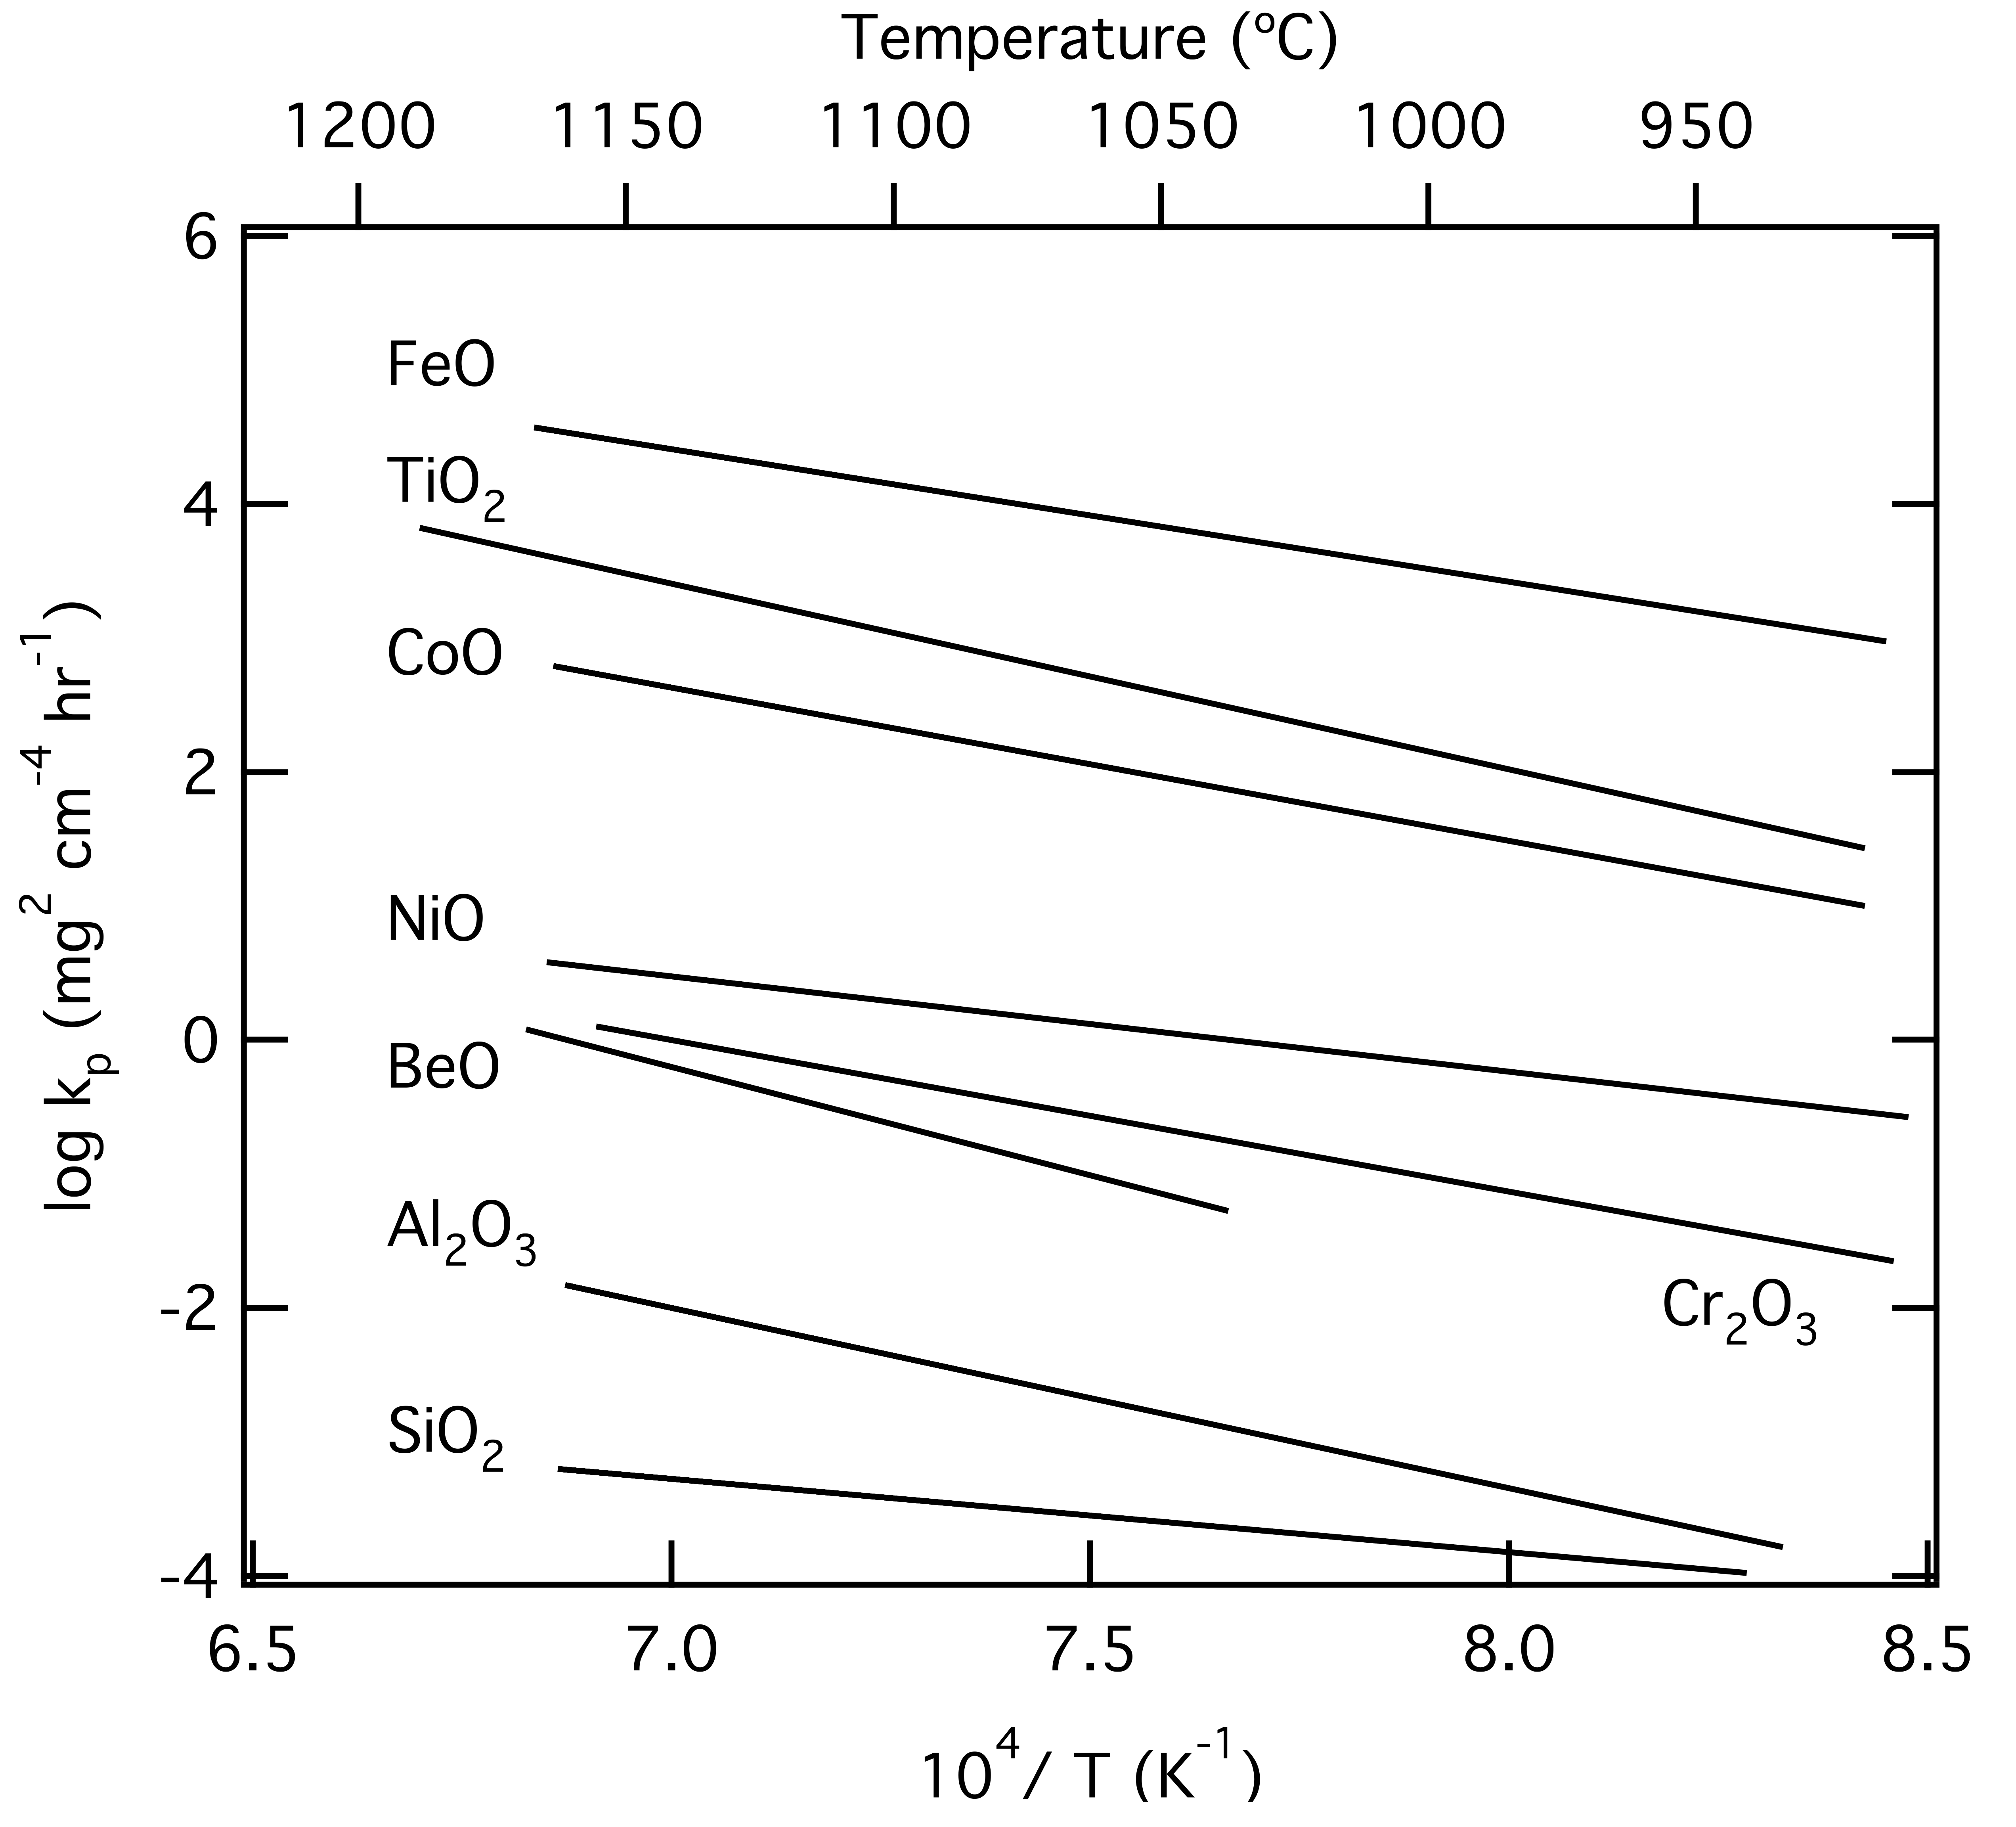
\includegraphics[width=11cm]{oxides}
\caption{The permeability of oxygen through various oxides vesus temperature ~\cite{nesbitt93}.}
\label{fig:oxidepermeability}
\end{center}
\end{figure}
%

\section{PGM Superalloys}

An extension of superalloy development based on platinum-group metals (PGMs) such as platinum, iridium and rhodium has been performed ~\cite{wenderoth05, mitarai98, mitarai97, mitarai99}.  These alloys are similar to nickel-base superalloys, and have a solid-solution matrix with a loading-bearing intermetallic L1$_2$ phase (Figures \ref{fig:ir17nb}).  The eutectic temperature between Ir solid-solution and Ir$_3$Nb is very high, at 2400\celsius\ (Figure \ref{fig:irnb}).  Casting this composition would be beyond the capabilities of most directional solidification (DS) facilities.  

The labyrinth structure of Ir-15at.\%Zr is similar to superalloys designed with very high misfit.  In Figure \ref{fig:LDSXInterrupted}, the microstructure of LDSX 8, a highly-misfitting superalloy, has many similarities to Ir-15at.\%Zr (Figure \ref{fig:ir17nb}b).  Such alloys have higher melting points than nickel-base superalloys and have the potential to operate at temperatures that are several hundred degrees higher than current superalloys ~\cite{okamoto94ir}.  

This alloy design approach has met with some success.  For instance, the 0.2\% flow stress of a binary PGM superalloy reached 1400  \mega\pascal\ at 1200\celsius\ (Figure \ref{fig:ir17nbi}) ~\cite{mitarai99}.  On the other hand, these alloys are three times denser than nickel-base superalloys and are also prohibitively expensive. 

 Although their densities make them unsuitable for moving parts, they may be well-suited for projects that operate on an essentially unlimited budget, such as inter-planetary rocketry missions.  It would be difficult to justify the costs that would be incurred for use in commercial jet engines.  We believe that there are better development options available, and will not be exploring PGM superalloys further in this work. 


%
\begin{figure}[H]
\begin{center}
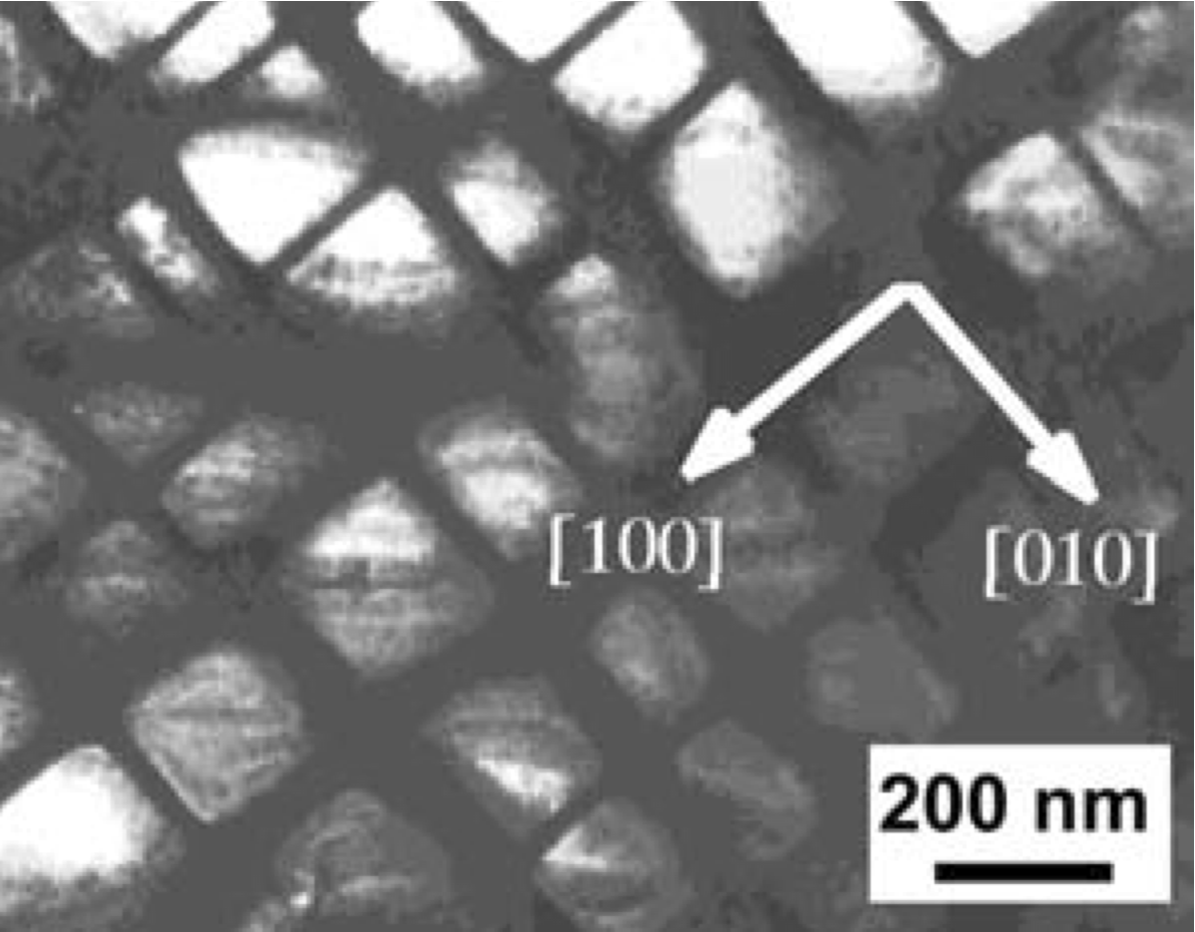
\includegraphics[width=7.2cm]{ir17nb}
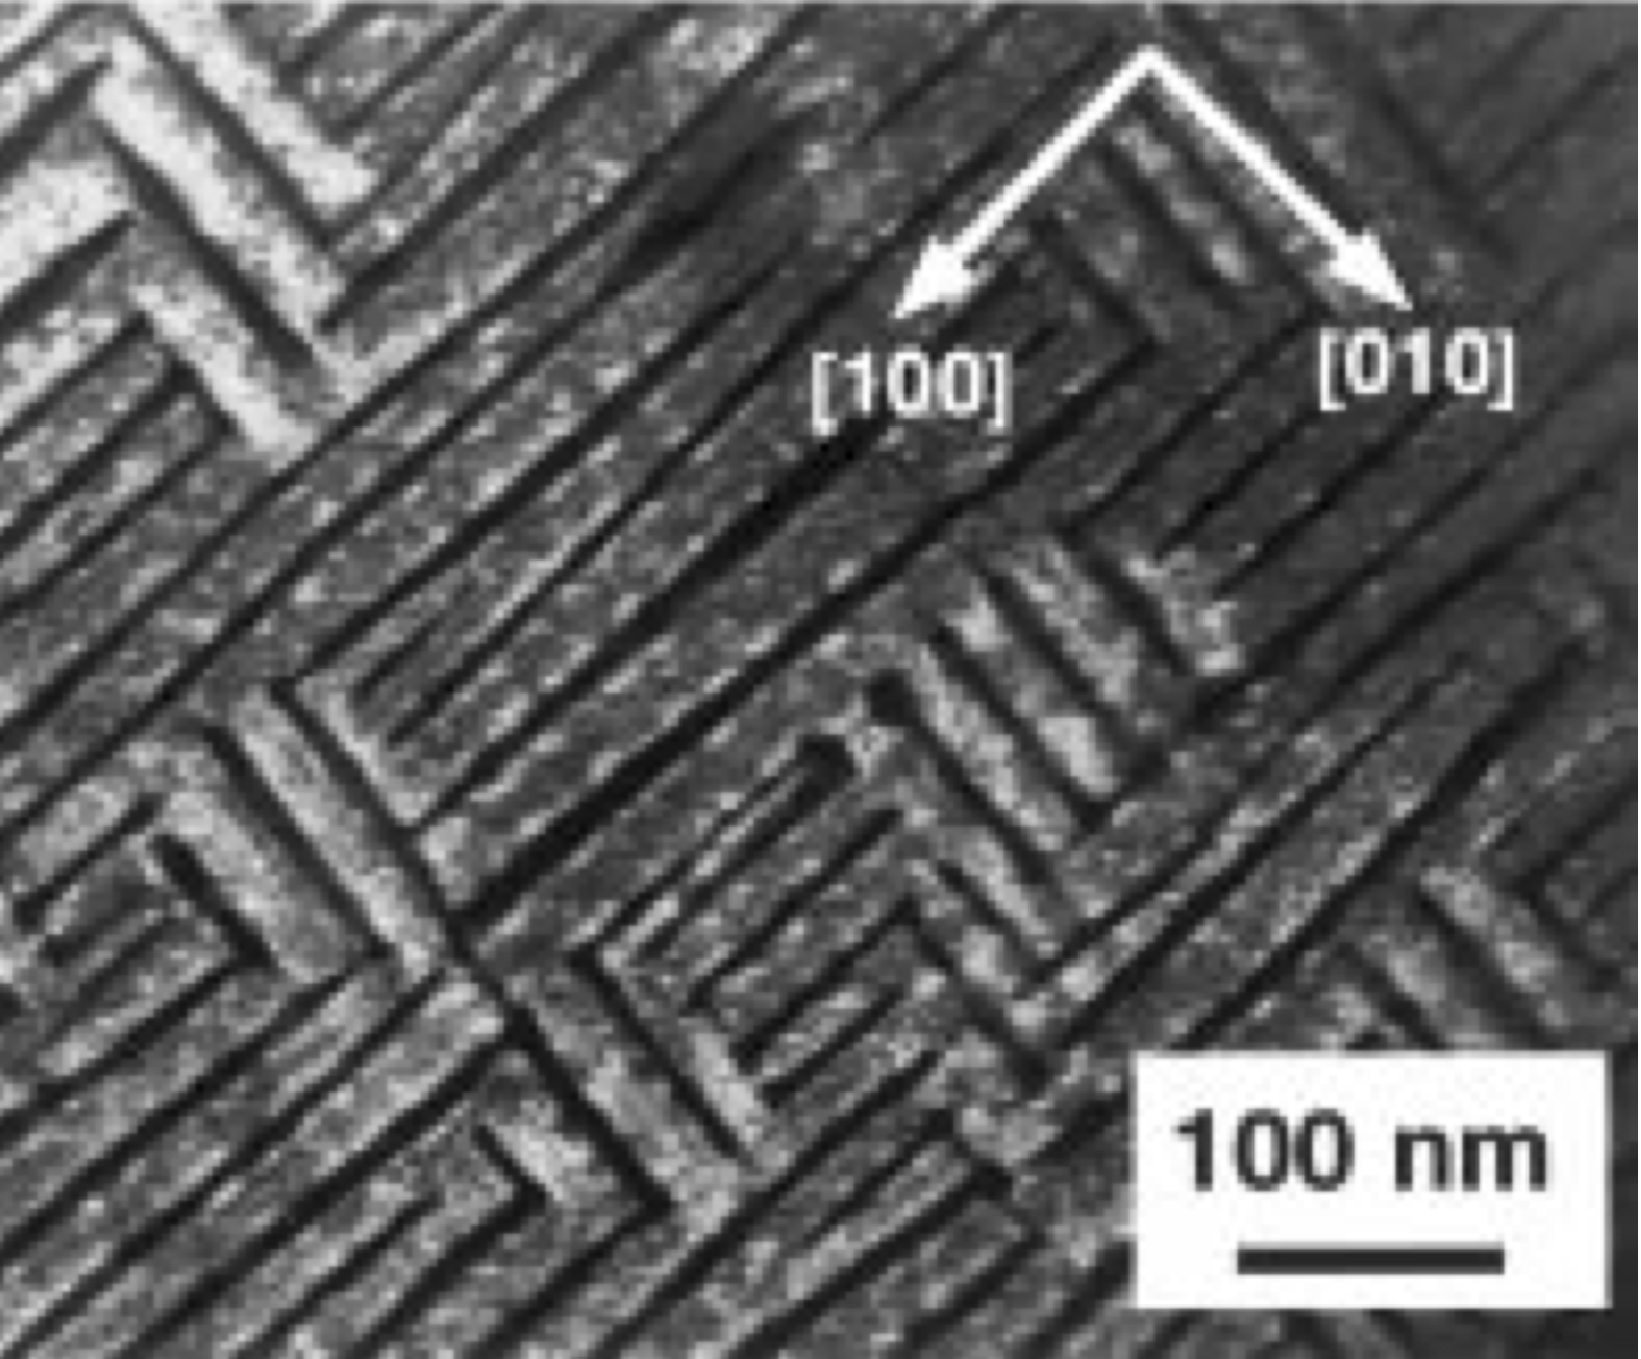
\includegraphics[width=6.75cm]{ir15zr}
\caption{(a) Microstructure of Ir-17Nb that has been heat treated at 1800\celsius\ for a day ~\cite{mitarai98}.  (b) Dark-field image of heat treated Ir-15at\% Zr, viewed from the [001] direction ~\cite{mitarai99}.}
\label{fig:ir17nb}
\end{center}
\end{figure}
%
%
\begin{figure}[H]
\begin{center}
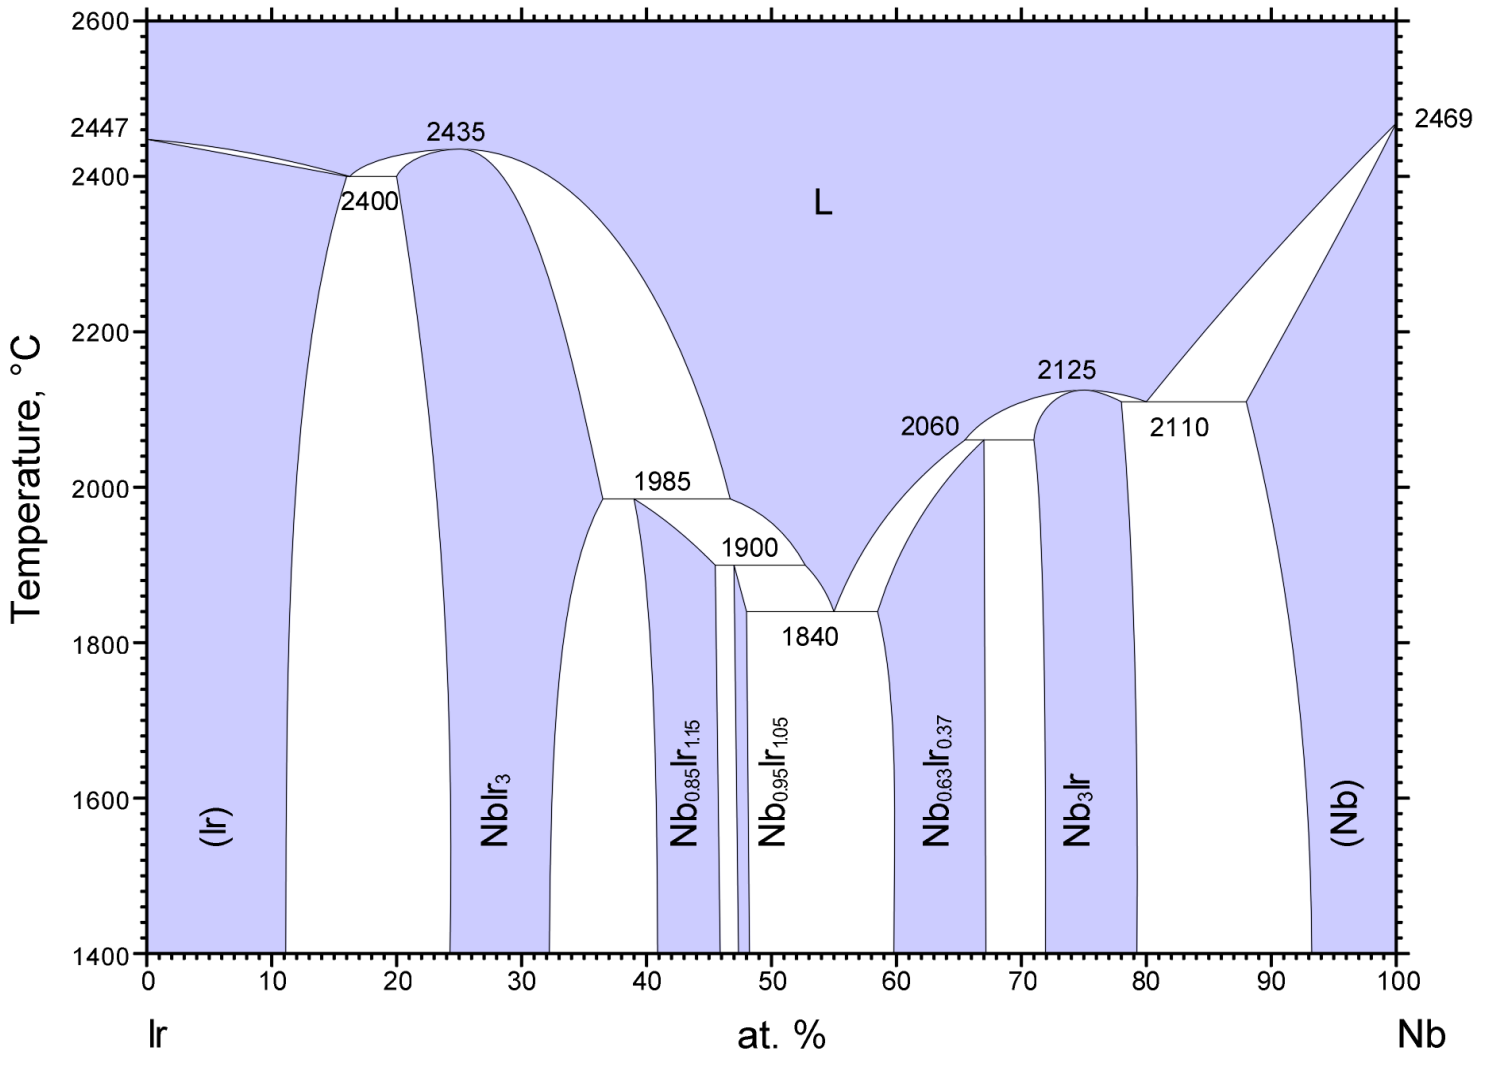
\includegraphics[width=16cm]{irnb}
\caption{Binary phase-diagram of Ir and Nb ~\cite{okamoto94ir}.}
\label{fig:irnb}
\end{center}
\end{figure}
%
%
\begin{figure}[H]
\begin{center}
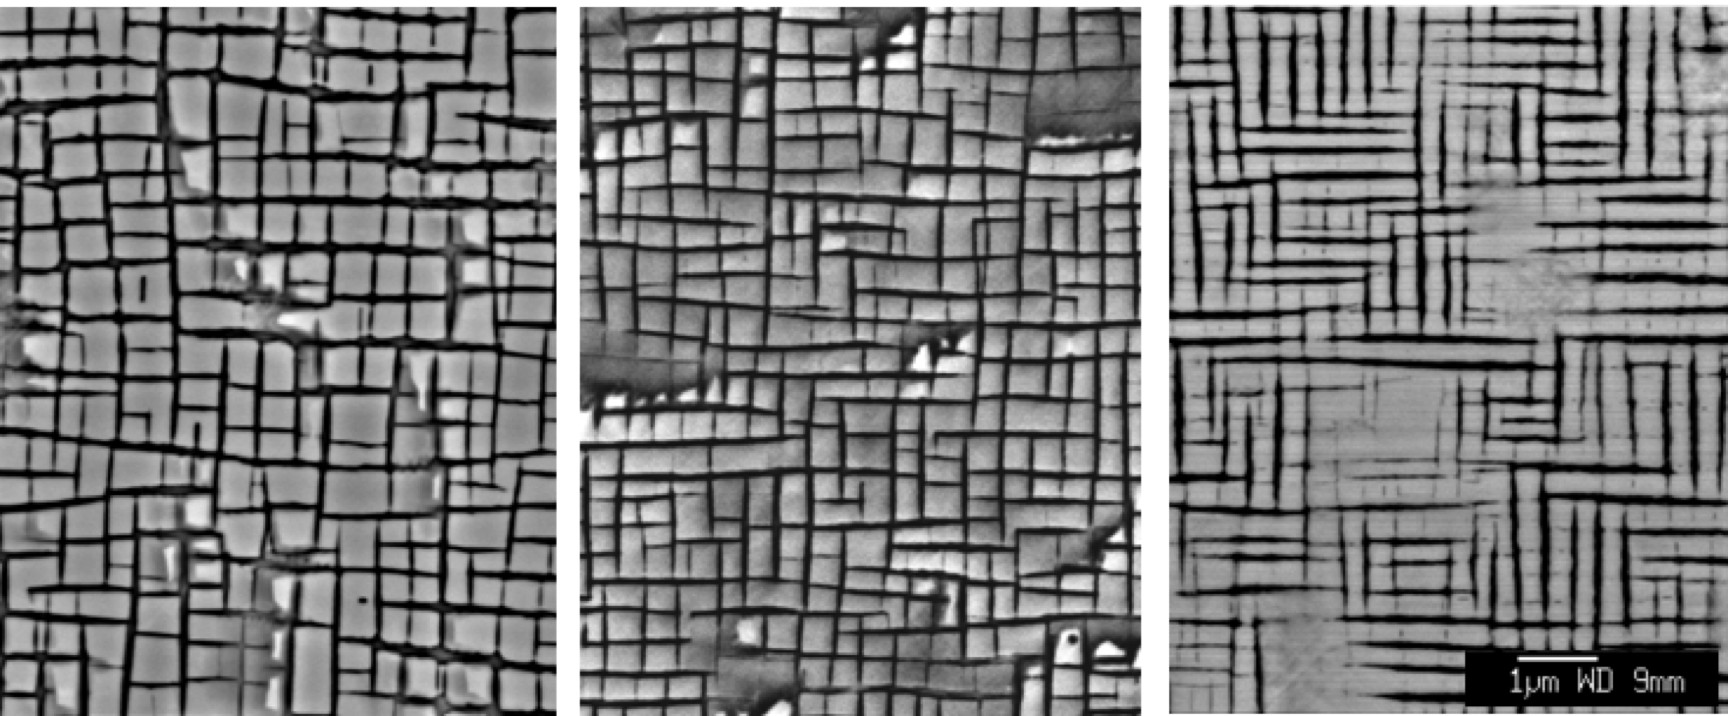
\includegraphics[width=16cm]{LDSXInterrupted}
\caption{Experimental nickel-based superalloys LDSX 1, 6 and 8.  They have increasing negative misfit from left to right.  These heat-treated specimens have been subject to tensile creep at 950\celsius/375 \mega\pascal.  The creep tests were stopped when the onset of secondary creep was observable.}
\label{fig:LDSXInterrupted}
\end{center}
\end{figure}
%
%
\begin{figure}[H]
\begin{center}
\includegraphics[width=8cm]{irflowstress}
\caption{0.2\% flow stresses of Ir alloys with -17at.\%Nb, -18Ta, -17Ti and -12Zr, when subject to compression tests at 1200\celsius\ ~\cite{mitarai99}.}
\label{fig:ir17nbi}
\end{center}
\end{figure}
%
\clearpage
\section{Alumina-Forming Alloys}

With the success enjoyed by nickel-based superalloys as high-temperature materials, there was a natural progression for research to concentrate on selected aluminides of nickel, titanium and iron in the 1980s and 1990s ~\cite{cotton93, miracle94a, walston93, white89, nathal92}.  

Ni$_3$Al and NiAl are the two nickel aluminides with melting-points higher than 1200\celsius\ (Figure \ref{fig:NiAl}) ~\cite{okamoto93}.  Ni$_3$Al is the intermetallic reinforcement phase in nickel-based superalloys.  It has a melting point of 1385\celsius, which is very close to the eutectic temperature of Ni--Ni$_3$Al.  In Figure \ref{fig:gpvolfrac}, an advanced single-crystal superalloy possessed the longest creep rupture life at 1000\celsius\ when it had a $\gamma$' volume fraction between 60-75\%.  This figure shows that the $\gamma$' volume fraction range for optimal creep performance of nickel-based superalloys is about 60--75\%  at temperatures between 780 and 1000\celsius.  A higher intermetallic content will not provide an increase in creep properties.  There is no benefit in designing an alloy without the toughening nickel solid-solution phase, as there would be no corresponding increase in high-temperature strength.

NiAl is a $\beta$2 phase with a melting point of 1638\celsius\ (Figure \ref{fig:NiAl}).  Its density of 5.92  \gram\usk\centi\rpcubic\meter\ is about 30\% lower than nickel-based superalloys ~\cite{okamoto93}.  The high-temperature properties of single-crystal and polycrystalline NiAl have been compared with Rene 80 in a Larson-Miller plot (Figure \ref{fig:NiAlLM}).  Rene 80 is a second generation nickel-based superalloy that is conventionally cast ~\cite{reed06}.  Single-crystal NiAl specimens outperform polycrystalline specimens at all temperatures tested, but both are vastly inferior to the third generation superalloy Rene80 (Figure \ref{fig:NiAlLM}). 

The anisotropic nature of DS-manufactured SX (single-crystal) NiAl can be seen in the differential in yield strength of NiAl grown in different orientations (Figure \ref{fig:NiAlys}) ~\cite{noebe96}.  The [100] orientation that shows superior strength at temperatures up to 400\celsius.  Above 400\celsius, [100] experiences a sharp reduction in yield strength.  The [110] orientation possess low yield strengths of 50--150MPa when above 100\celsius.  The [123] orientation has a slightly higher yield stress of 350-500 \mega\pascal\ above 200\celsius.  The orientation dependence of the yield stress arises because the normal slip systems are <100>\{010\}  and they cannot contribute to deformation along <100> because the resolved shear stress is zero on all such systems along <100>. Crystals stressed along <100> either kink, fracture or deform by operation of <111>\{110\} slip at low temperatures at very high stresses ~\cite{loretto71}.  The plastic deformation at these temperatures is associated with extensive dislocation climb because of the high concentration of thermal vacancies even at temperatures below 600\celsius\ ~\cite{fraser73a,fraser73b}.  These mid-to-high temperature properties are vastly inferior to superalloys.  The fracture-toughness of NiAl, like yield strength, is highest in the [100] direction ~\cite{kumar91}.

Alloying additions have improved mechanical properties at temperatures under 1000\celsius.  Co and Fe additions sit in the Ni-site of NiAl.  A Co content of about 40 at.\% increases NiAl creep resistance at 900\celsius\ most effectively across the Co and Fe contents tested (Figure \ref{fig:NiAlCo}) ~\cite{jung87}.  Other alloy additions such as Mo, the heusler phase and the TiB$_2$ phase have resulted in better high-temperature mechanical properties (Figure \ref{fig:NiAlLM}) ~\cite{miracle94a, walston93, darolia93, polvani76}, but due to the substantial softening at relative low temperatures of about 400\celsius, NiAl alloys have not been found to offer a mechanical advantage over superalloys at temperatures above 1100\celsius\ ~\cite{miracle94a}.
%
\begin{figure}[H]
\begin{center}
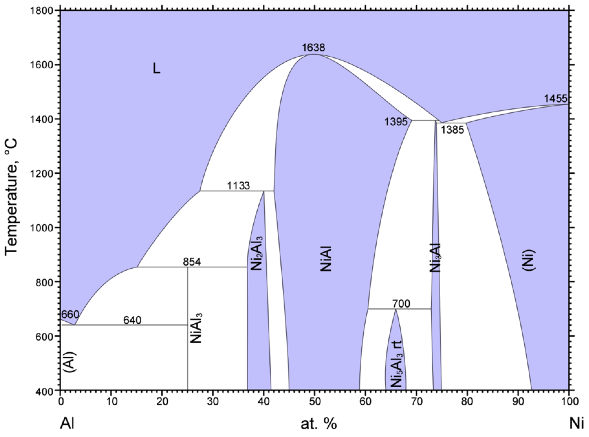
\includegraphics[width=14cm]{NiAl}
\caption{Binary phase-diagram of Ni and Al ~\cite{okamoto93}.}
\label{fig:NiAl}
\end{center}
\end{figure}
%
%
\begin{figure}[H]
\begin{center}
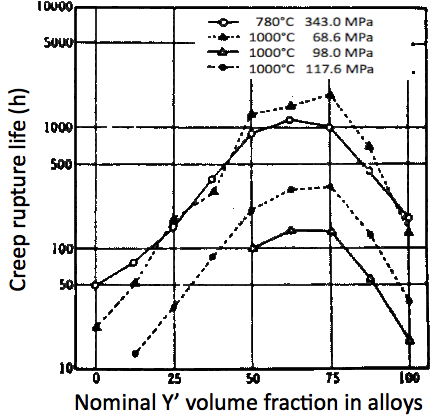
\includegraphics[width=10cm]{gpvolfrac}
\caption{Creep rupture life versus $\gamma$' volume fraction in an advanced single-crystal nickel-based superalloy, at 780\celsius/343MPa, and 68.6MPa, 98.0MPa and 117.6MPa at 1000\celsius\ ~\cite{harada82}.}
\label{fig:gpvolfrac}
\end{center}
\end{figure}
%

%
\begin{figure}[H]
\begin{center}
\includegraphics[width=15cm]{NiAlLM}
\caption{Rupture stress versus the Larson-Miller parameter for poly-crystalline and single-crystal NiAl, together with four other NiAl alloys.  Nickel-based superalloy Rene80 has been used as a bench-mark alloy ~\cite{walston93}.}
\label{fig:NiAlLM}
\end{center}
\end{figure}
%
%
\begin{figure}[H]
\begin{center}
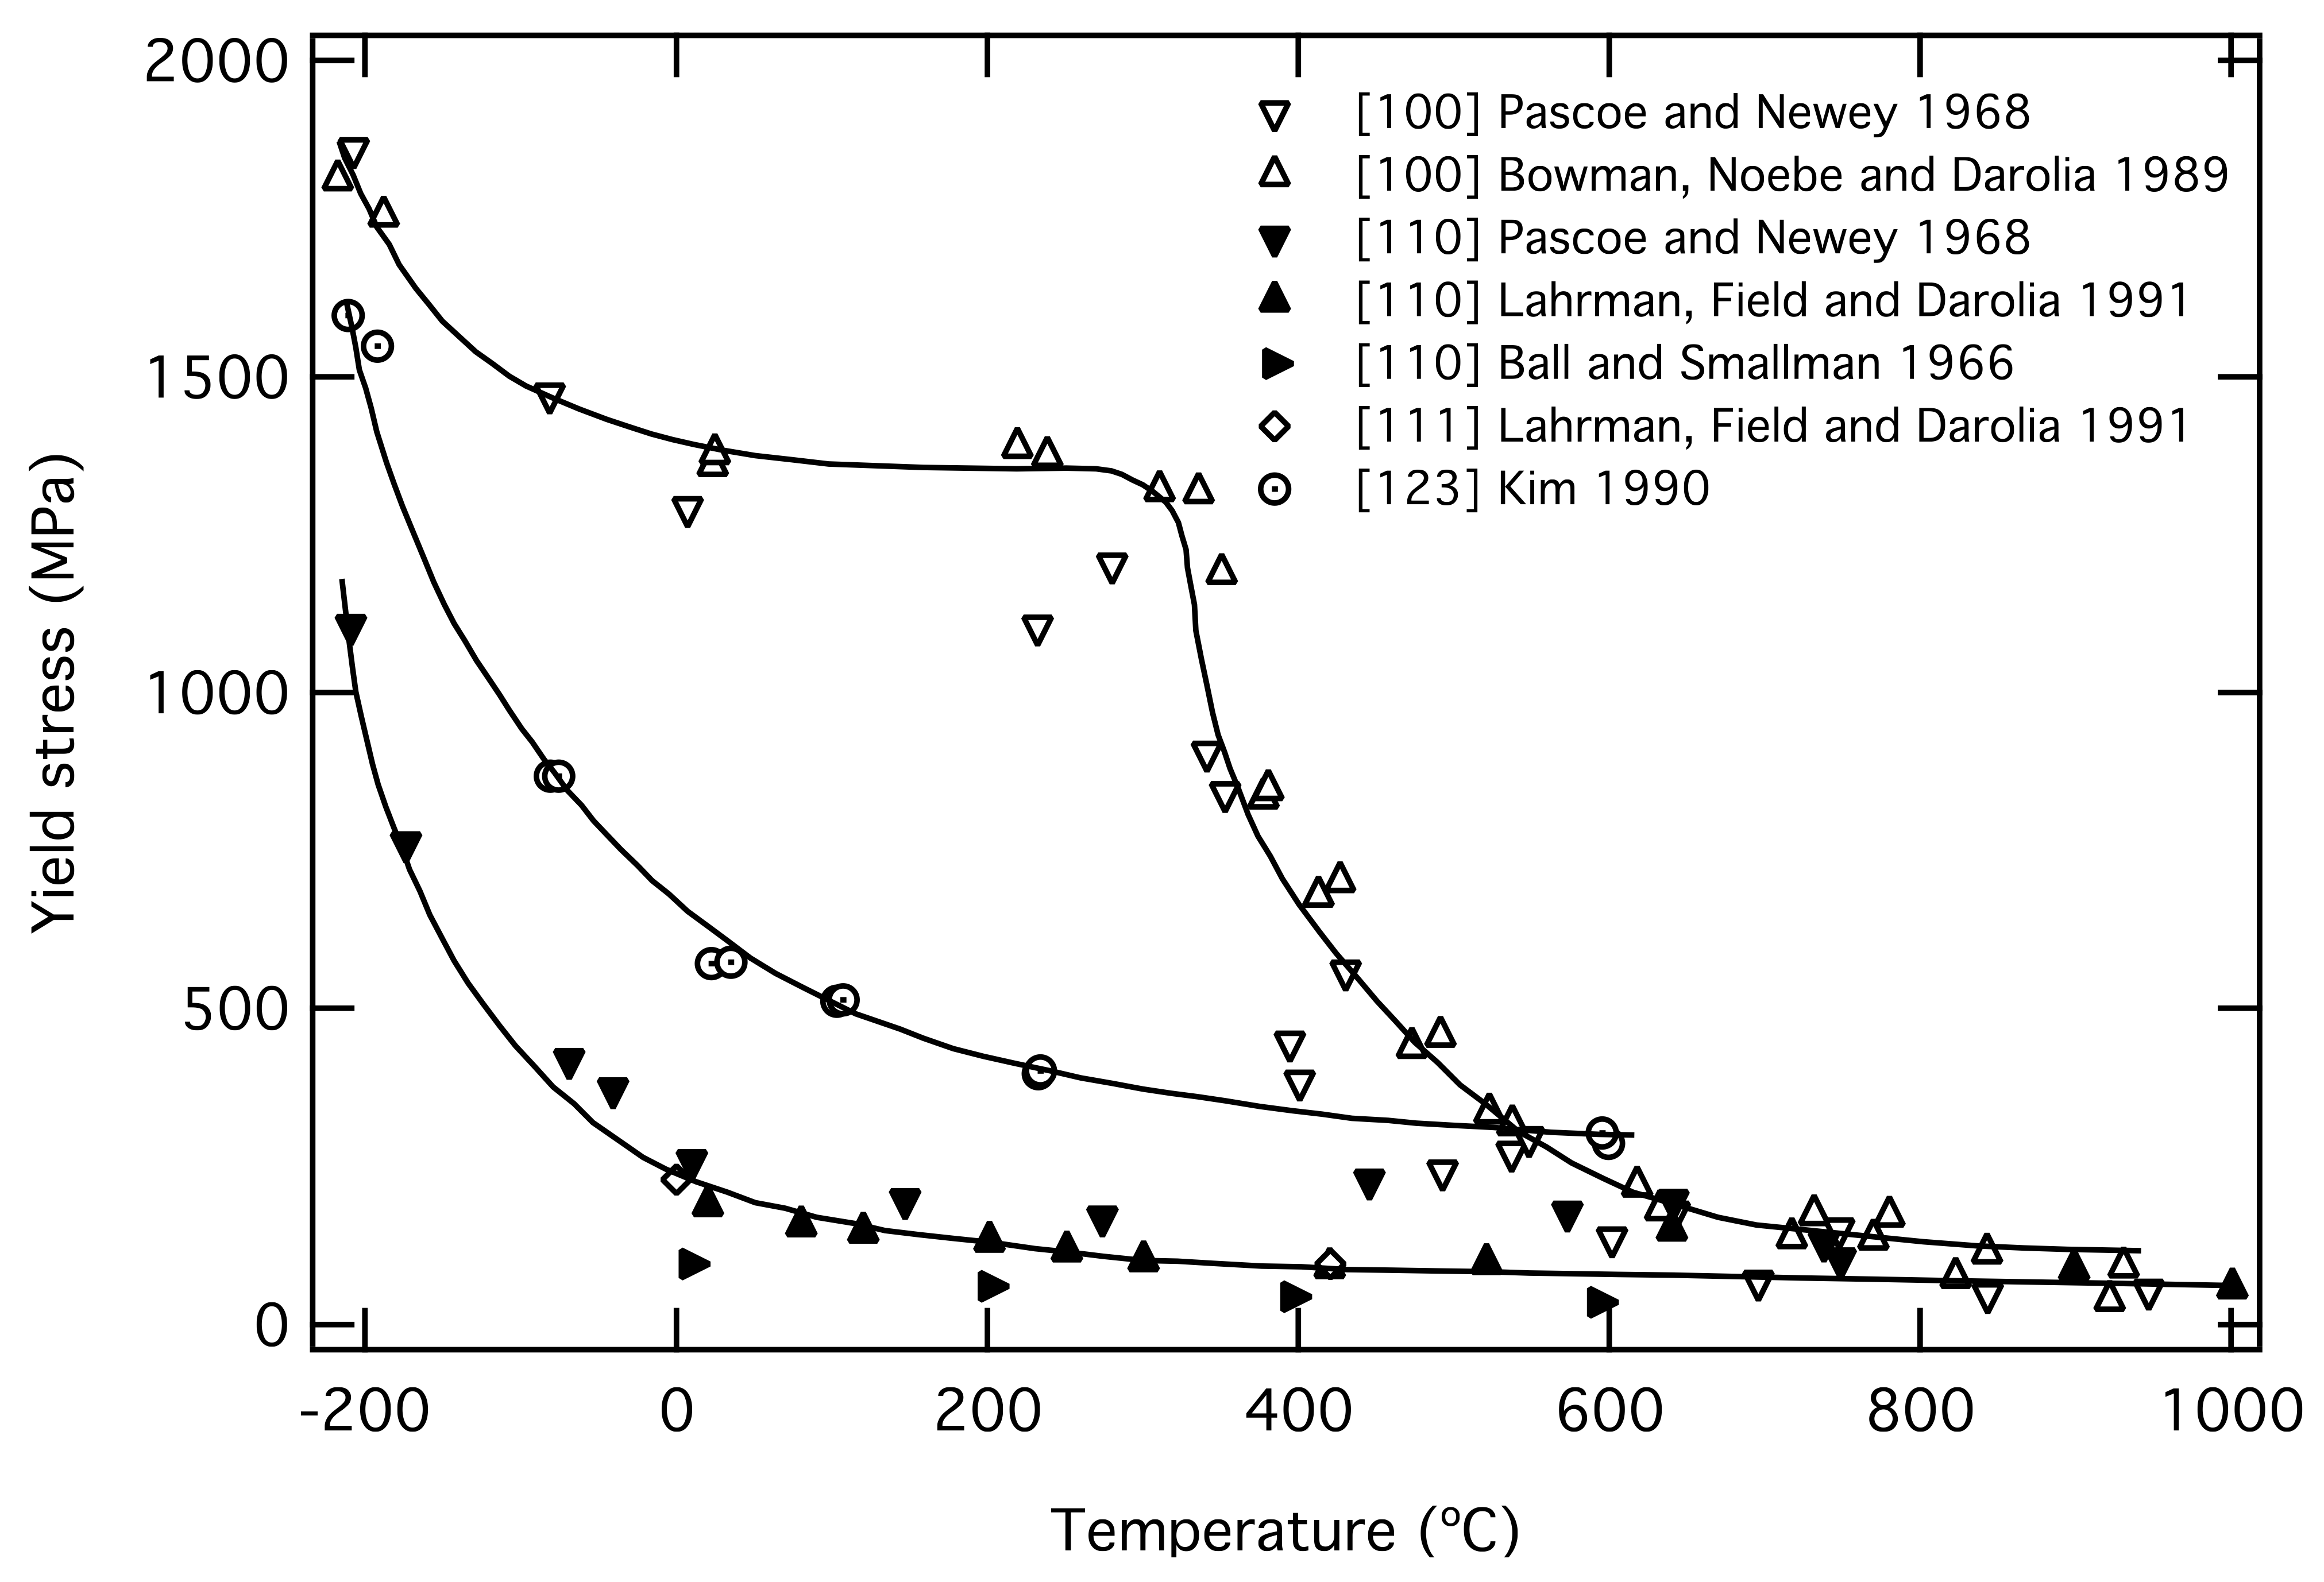
\includegraphics[width=15cm]{NiAlys}
\caption{The yield stresses for the main orientations of NiAl between -200\celsius\ and 1000\celsius\ ~\cite{noebe96}.}
\label{fig:NiAlys}
\end{center}
\end{figure}
%
%
\begin{figure}[H]
\begin{center}
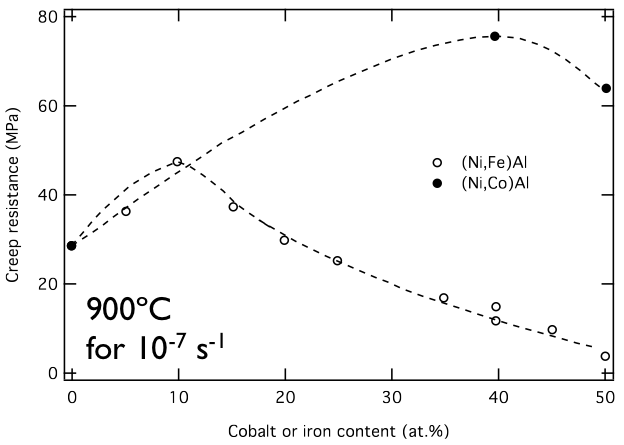
\includegraphics[width=12cm]{NiAlCo}
\caption{Creep resistances of (Ni,Fe)Al and (Ni,Co)Al at a creep-rate of 10$^{-7}$s$^{-1}$ at 900\celsius\ ~\cite{jung87}.}
\label{fig:NiAlCo}
\end{center}
\end{figure}
%

 
In Figure \ref{fig:LMplotforintermetallics}, the stress required for 1\% deformation versus log time has been plotted for various intermetallics and their constituent elements.  Single-crystal PWA 1480 has been used as bench-mark.  Nb$_2$Al (black square), the Nb aluminide with the higher Al content, is more creep resistant than Nb$_3$Al (upright white triangle) at 184MPa/1000\celsius.  The former would also have better resistance against `pesting' due to its higher Al content.

In Figure \ref{fig:darolia96}, the specific creep strength at a low temperature of 1027\celsius\ for SX, polycrystalline and eutectic (coupled with Ni solid-solution) NiAl have been plotted.  NiAl, when manufactured to give high strength, has inadequate fracture-toughness for aerofoil applications ~\cite{darolia96}.

The only high-temperature aluminide in the Co--Al binary is CoAl (Figure \ref{fig:coal}).  It has a melting point of 1640\celsius\ and a low density of 6.07 \gram\usk\centi\rpcubic\meter.  It is creep resistant at temperatures of 1000\celsius\ and below ~\cite{anton89, jung87}, and is unsuitable for higher temperature applications.  

%
\begin{figure}[H]
\begin{center}
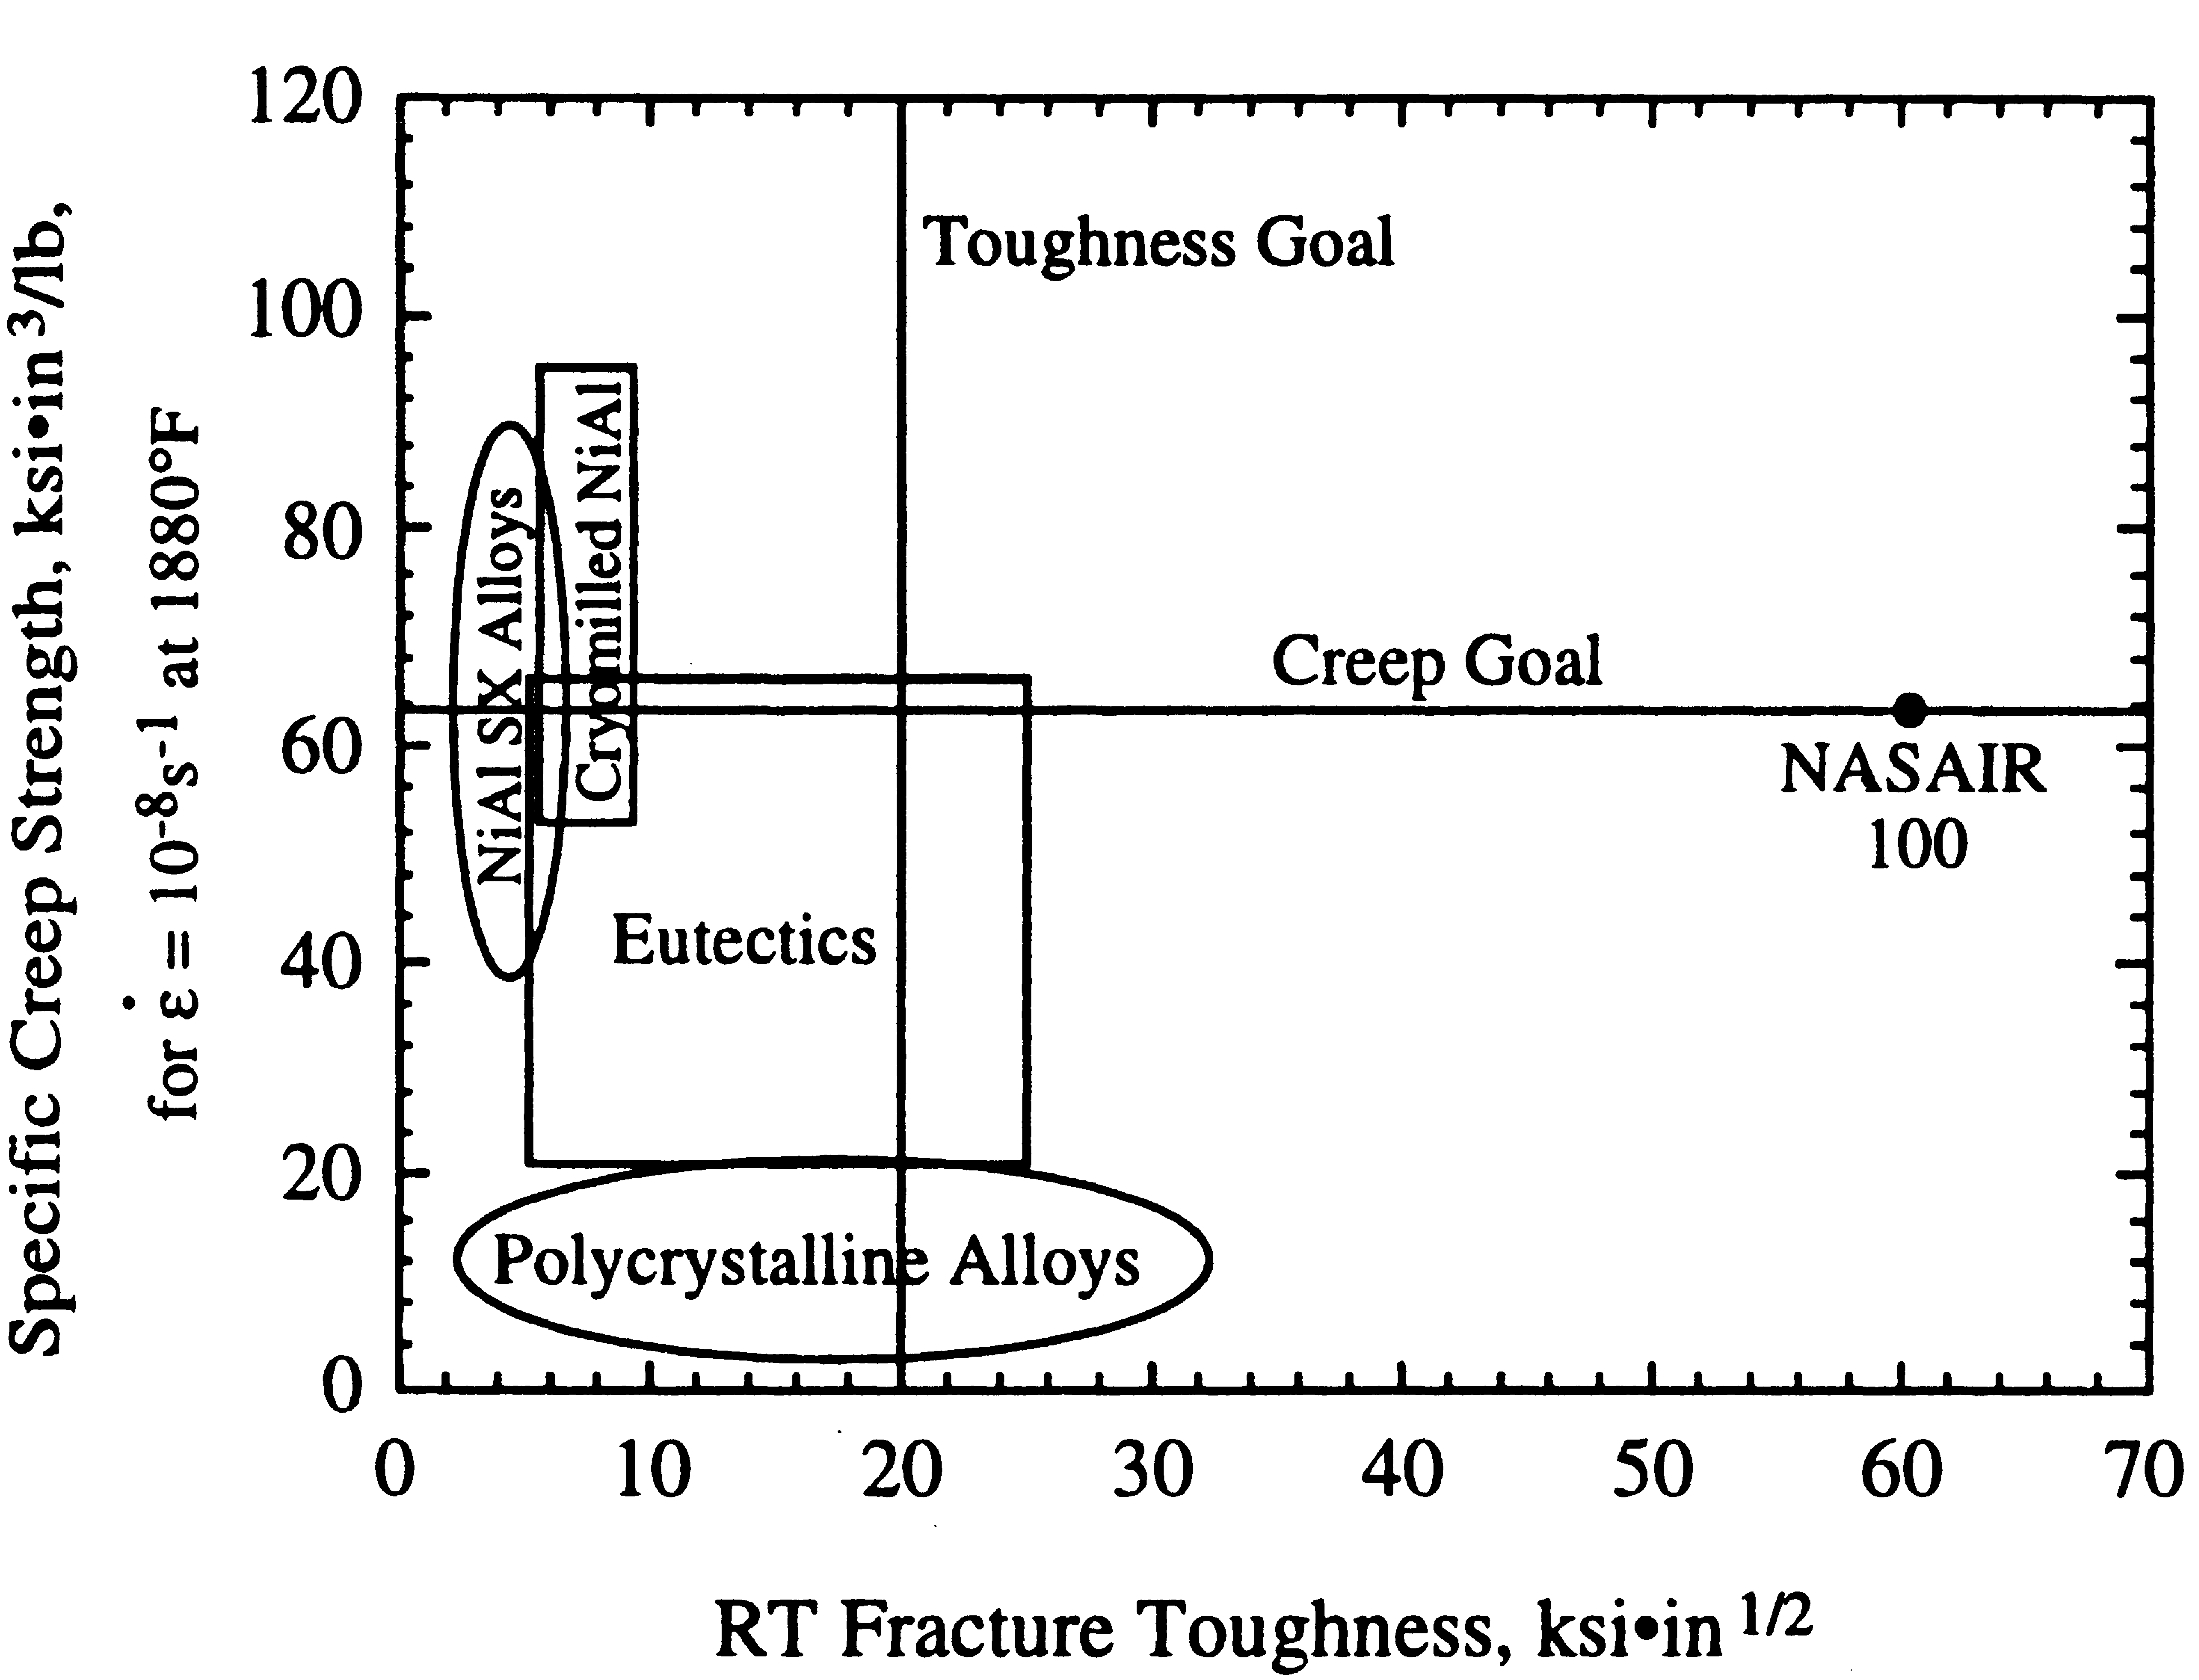
\includegraphics[width=13cm]{darolia96}
\caption{Specific creep strength versus fracture-toughness for several classes of materials considered for high-temperature application ~\cite{darolia96}.}
\label{fig:darolia96}
\end{center}
\end{figure}
%

%
\begin{figure}[H]
\begin{center}
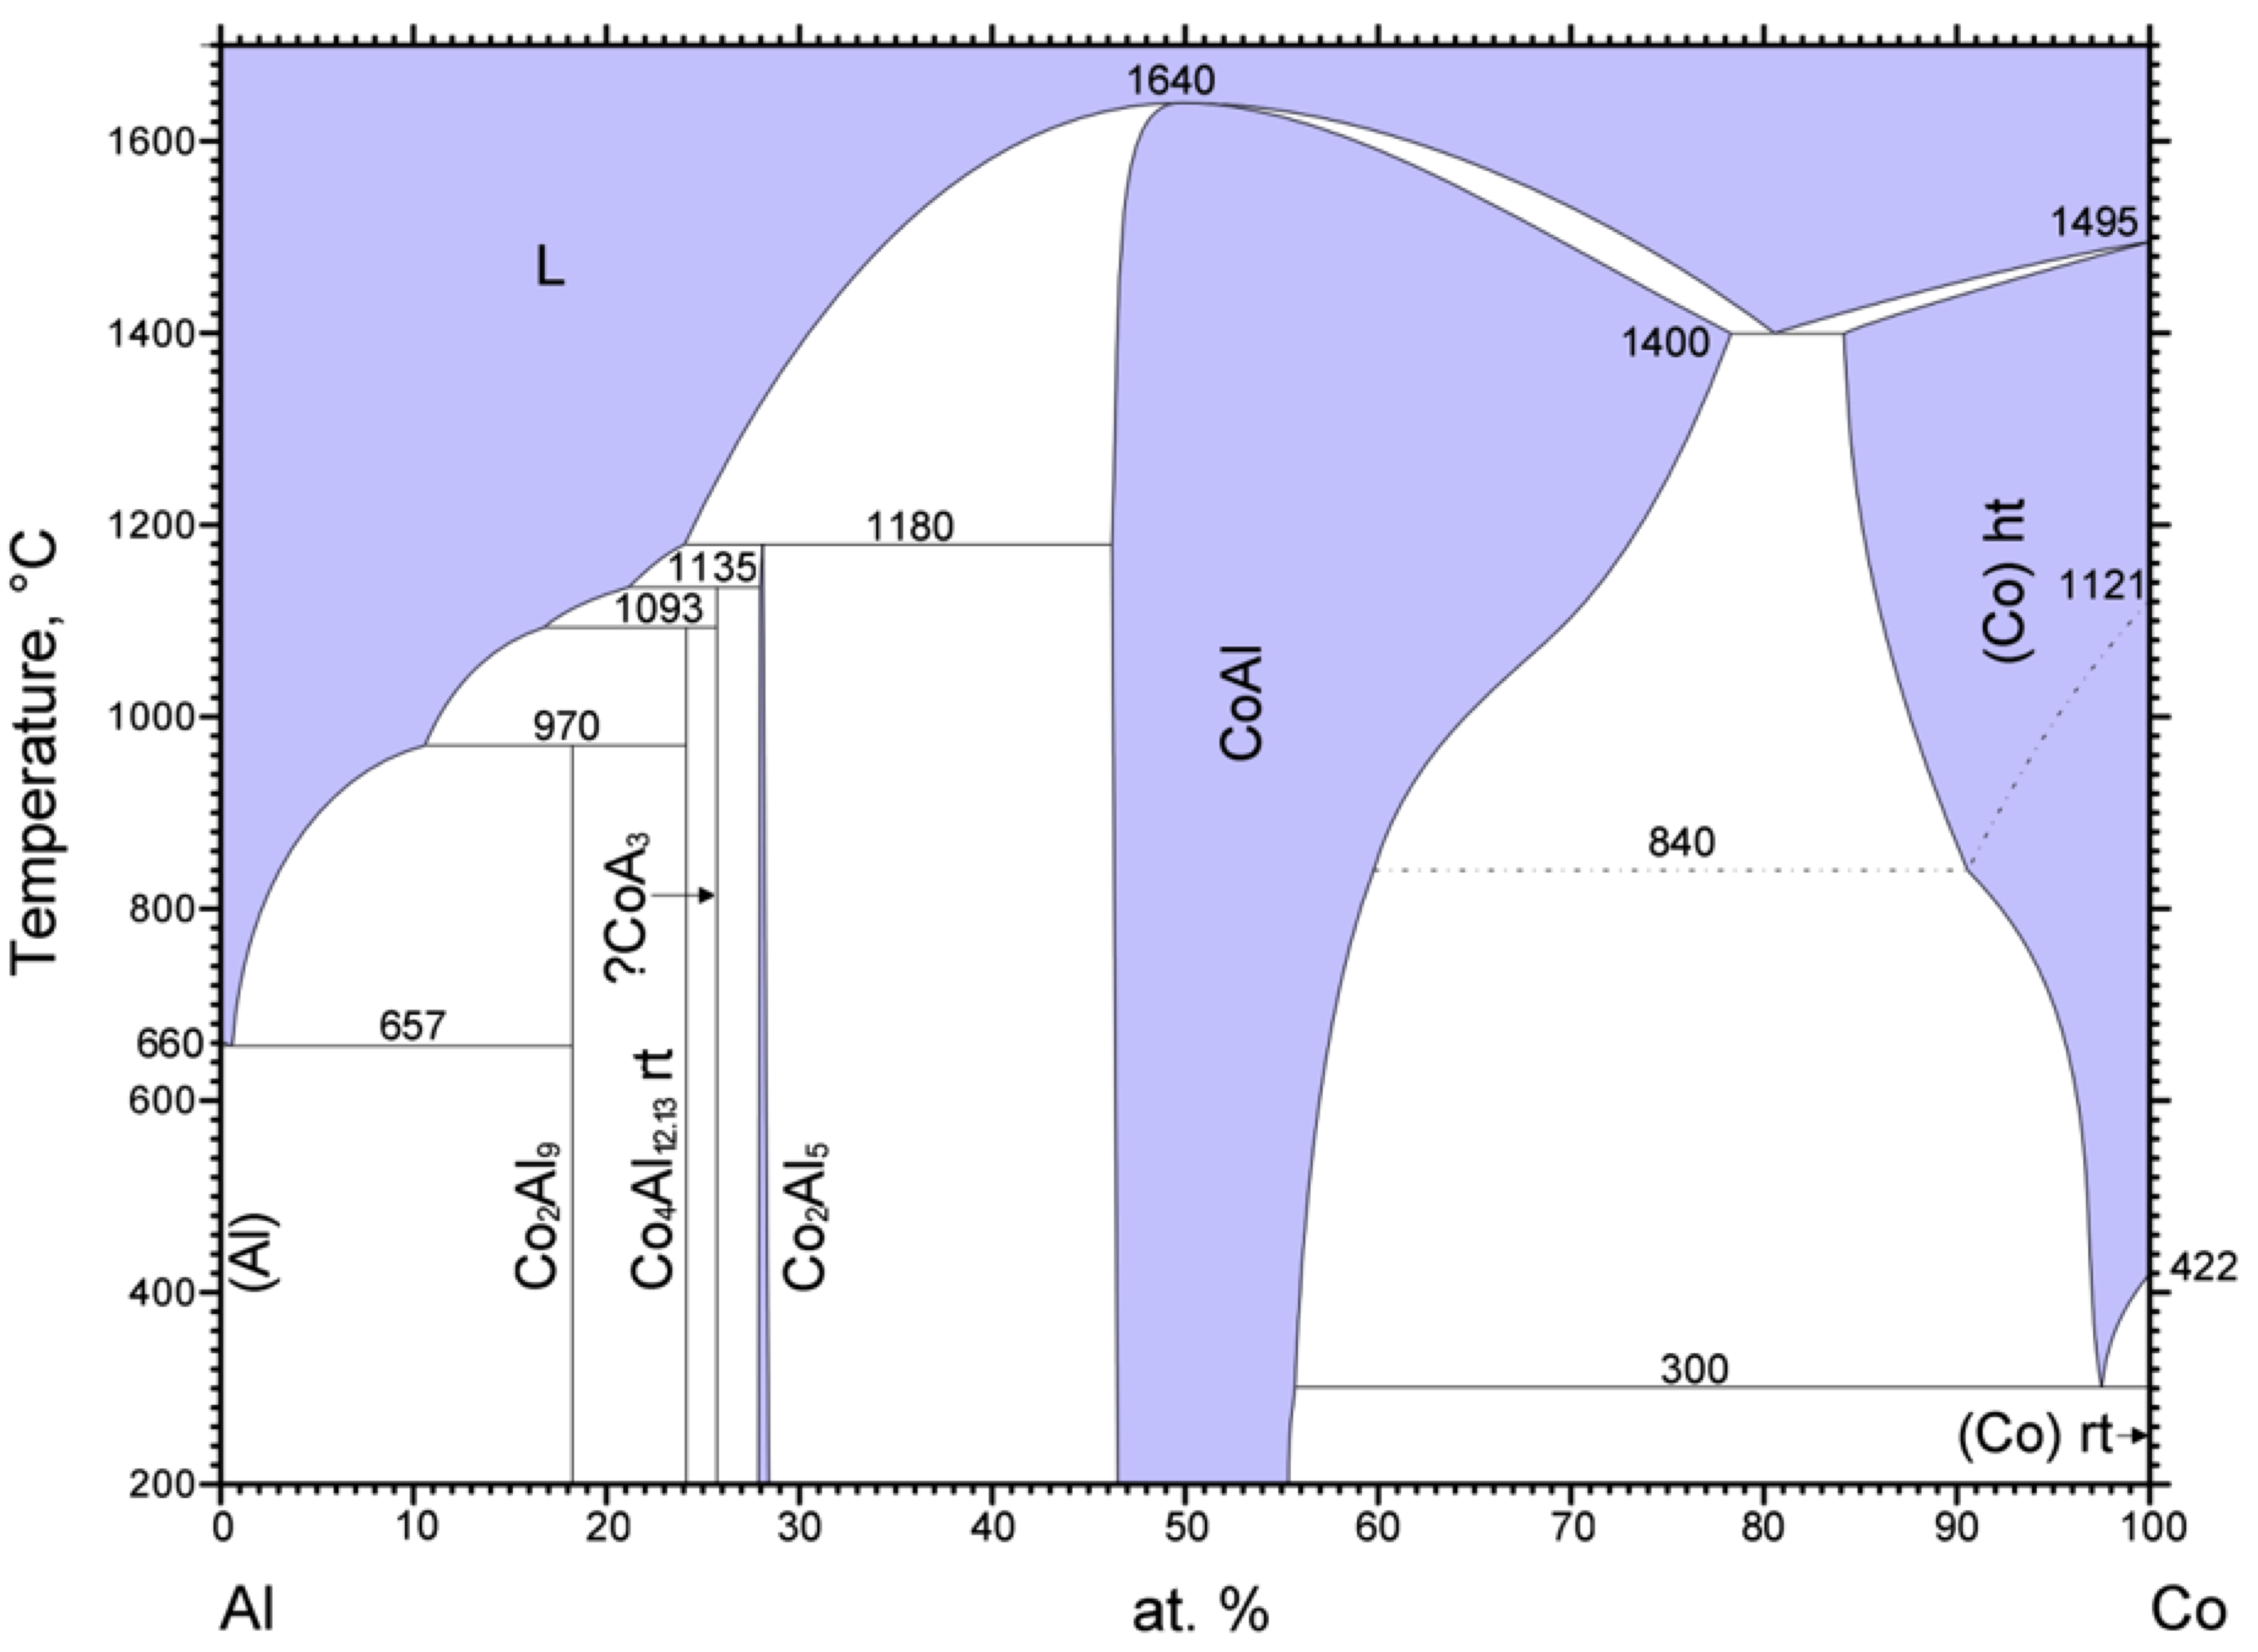
\includegraphics[width=14cm]{coal}
\caption{Binary phase-diagram of Co and Al~\cite{mcalister90}.}
\label{fig:coal}
\end{center}
\end{figure}
%


%
\begin{figure}[H]
\begin{center}
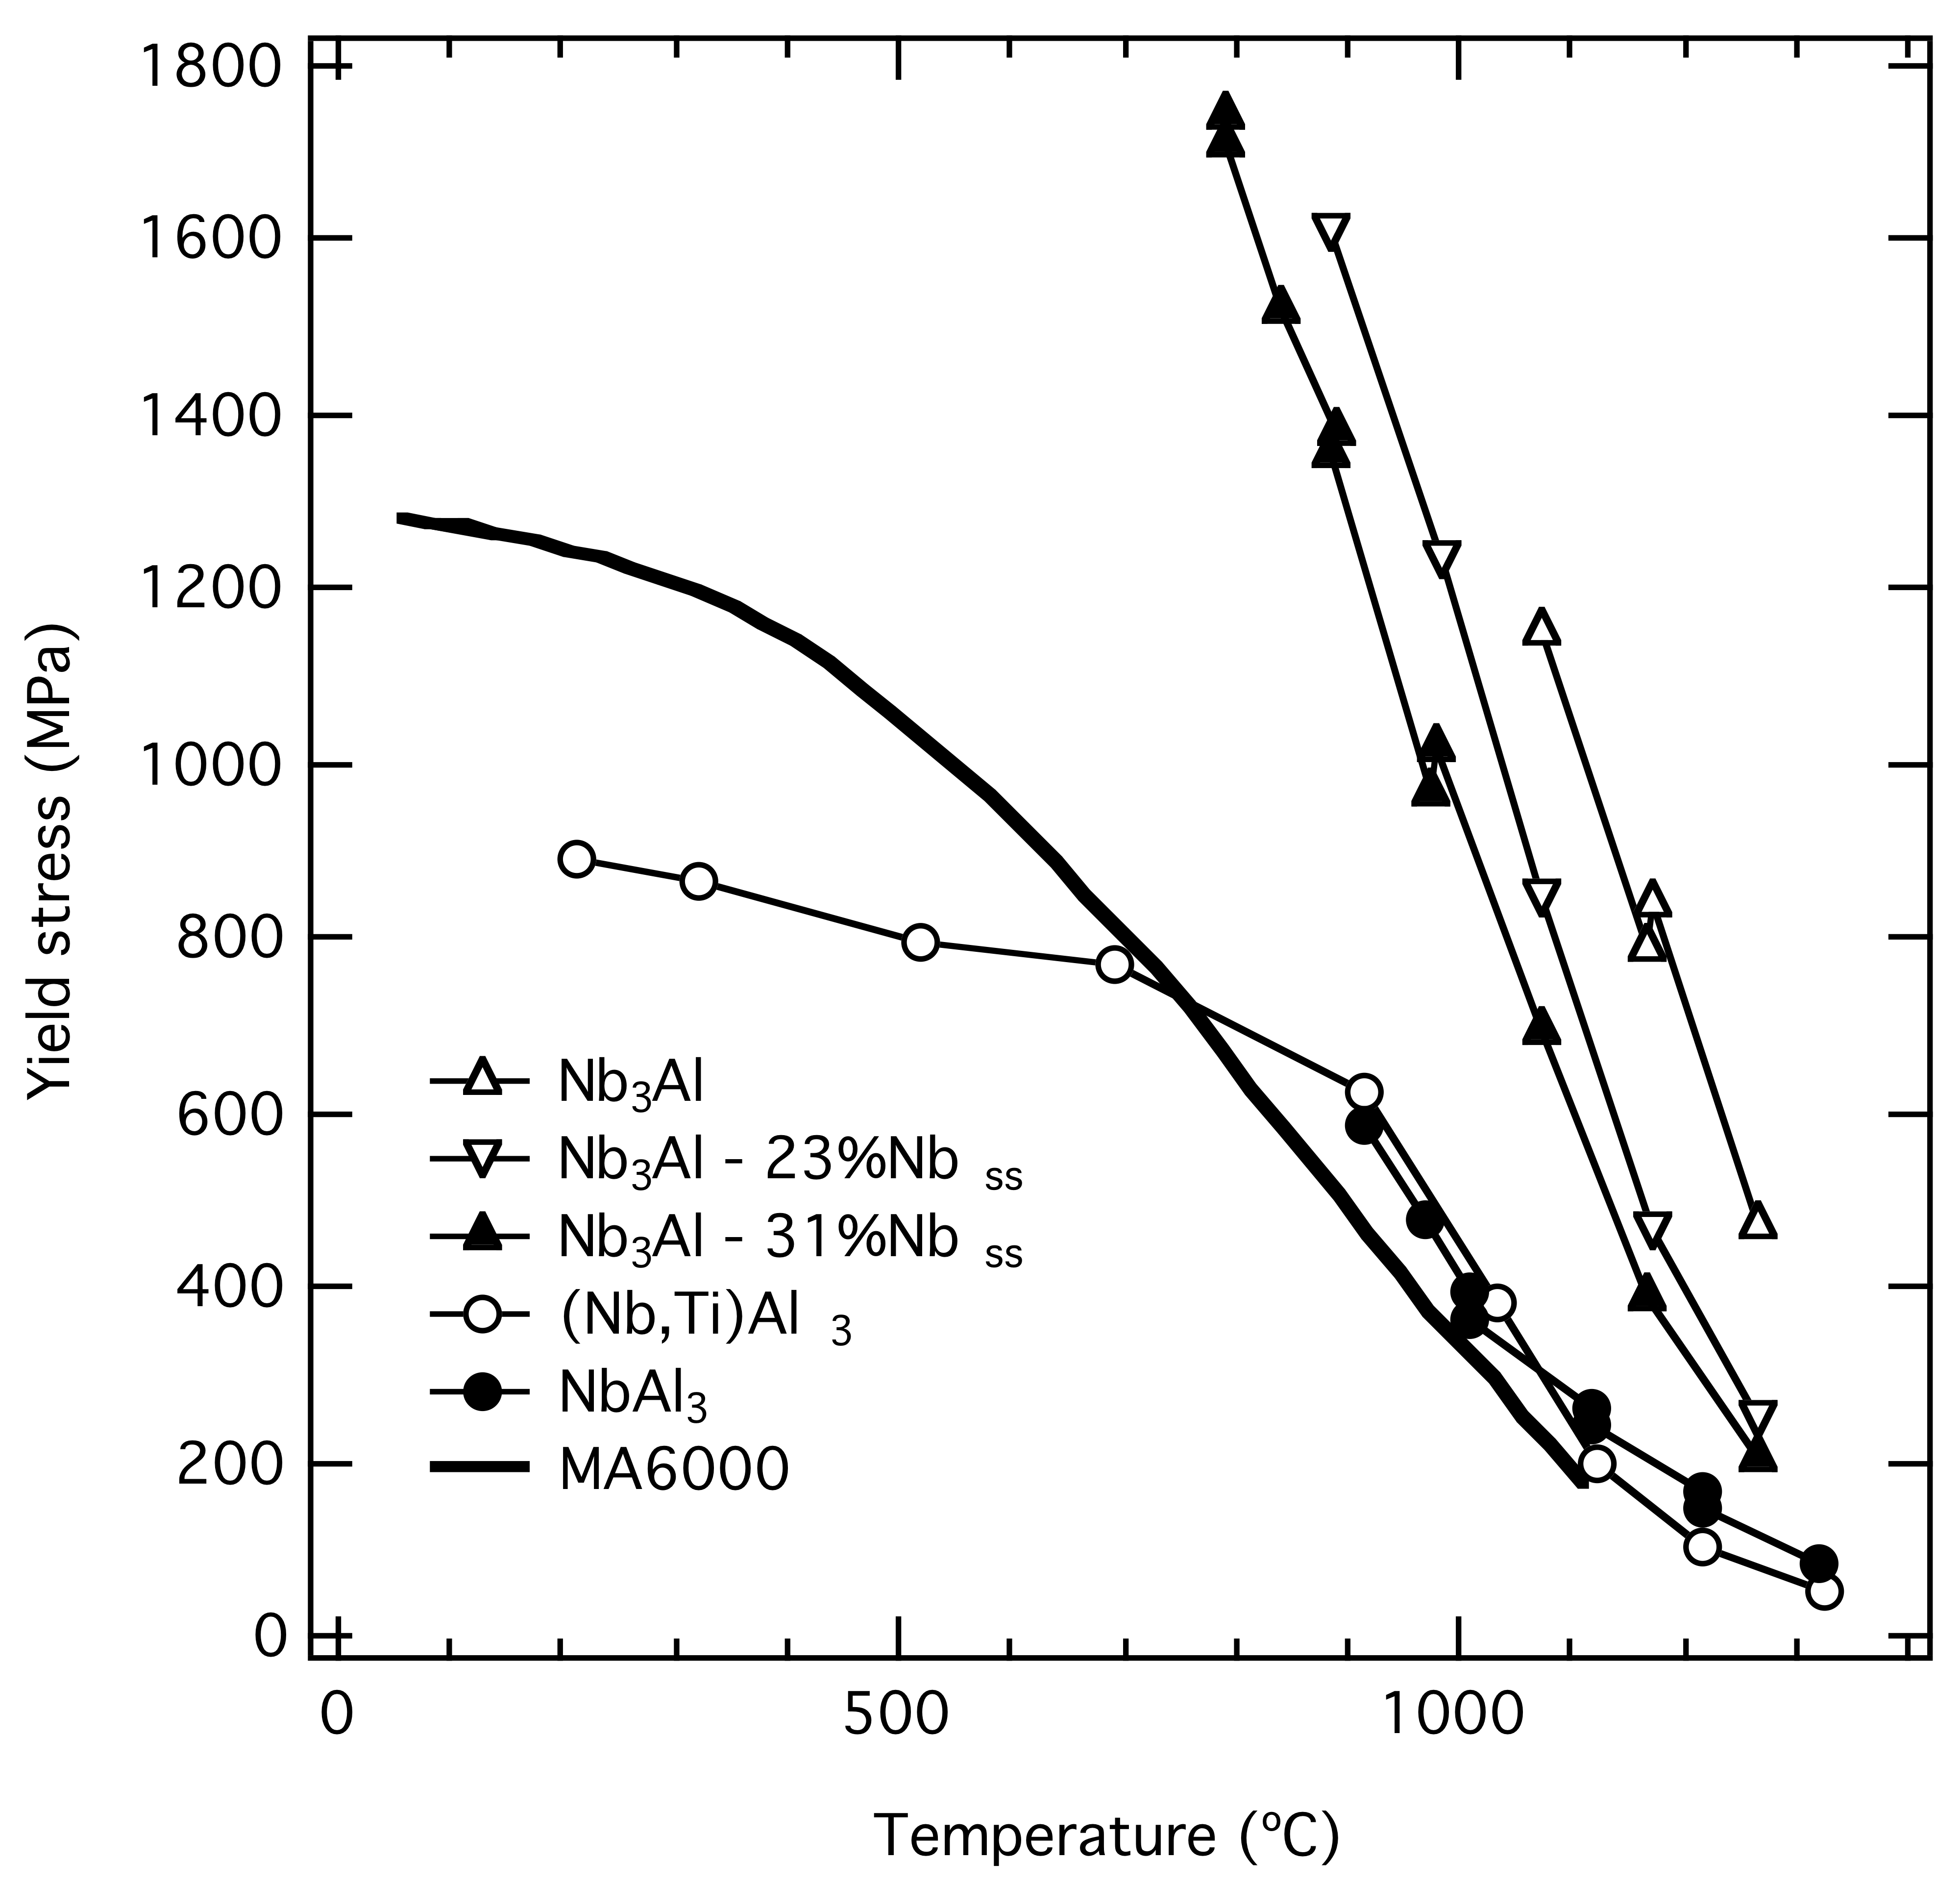
\includegraphics[width=10cm]{nbalys}
\caption{Yield strength of Niobium aluminides between room temperature and 1400\celsius.}
\label{fig:nbalys}
\end{center}
\end{figure}
%
Niobium aluminides have also been explored.  They show good high-temperature properties (Figure \ref{fig:nbalys}) up to about 1100\celsius.  Pure Nb$_3$Al has the highest yield strength at 1250\celsius, but it has poor oxidation resistance due to the formation of non-protective, volatile niobium pentoxide and AlNbO$_4$ during high-temperature exposure.  The Al content is not high enough to allow the alloy to form a protective alumina layer.  It is also susceptible to `pesting'.  Pesting is wide-scale, catastrophic, runaway oxidation of alloys at intermediate temperatures.  This occurs in many alloys containing Mo and Nb \cite{bewlay03, nesbitt93, ochiai06, shah92}.  Alloys that pest would experience uncontainable, uncontrollable, through-specimen oxidation in several hours.  Remnant alloy would not be found.  Pesting is many orders of magnitudes worse than the localised oxidation that has been seen in the latest generation nickel-based superalloys. Such localised oxidation would only extend 100\micro\metre\ from the original alloy surface; pesting, when it occurs, stops only when there is no alloy left that can be oxidised.


%
\begin{figure}[H]
\begin{center}
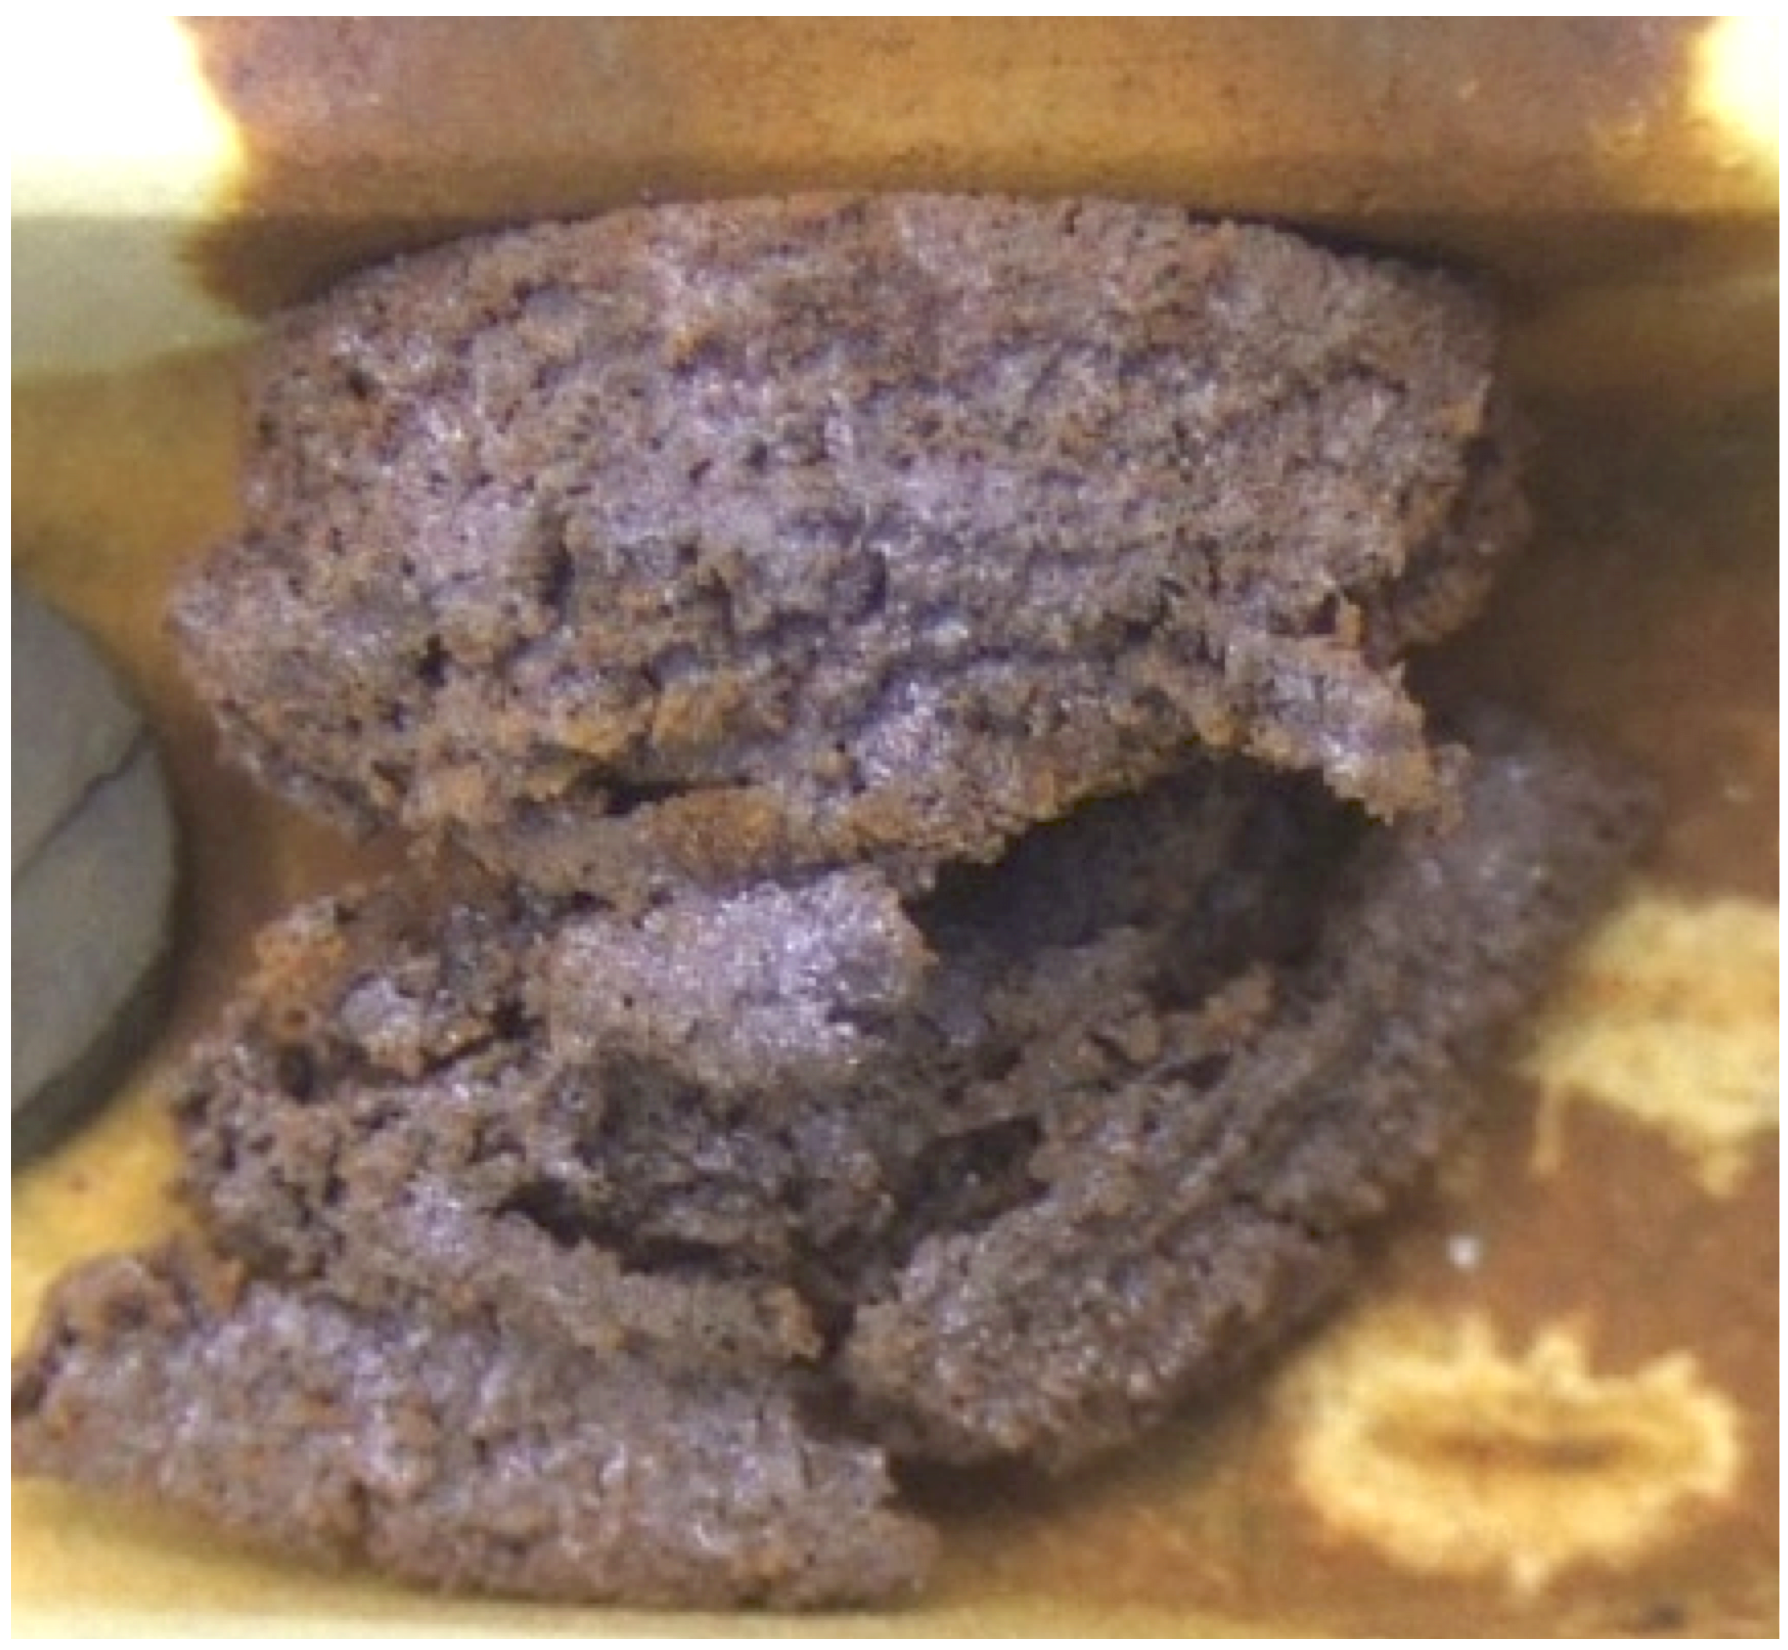
\includegraphics[width=5cm]{pest}
\caption{Pesting of a V--V$_3$Si alloy after 10 hours at 800\celsius.}
\label{fig:pest}
\end{center}
\end{figure}
%

Essentially, extensive efforts undertaken to improve the high-temperature mechanical properties of aluminides did not lead to increases in creep resistance.  They are believed to be unlikely to achieve higher temperature capabilities than nickel-base superalloys.


\section{Chromia-Forming Alloys}

Chromium oxide is known to be excellent for corrosion resistance; in fact, the principal method for making stainless steels stainless is through its addition.  Chromium oxide, however, has the unfortunate characteristic of volatilising at temperatures above 950\celsius\ ~\cite{perez02}, and is typically deemed unsuitable as the means of protection for operating temperatures that are to exceed 1100\celsius.  High-temperature alloys that form a chromium oxide layer would need another non-permeable oxide layer to sit atop it, such as a silica layer.


\section{Silica-Forming Alloys}

Silicon dioxide is stable up to 1650\celsius\ ~\cite{hallstedt92}, which is substantially higher than the target temperature capability of 1200\celsius.  Its adhesion to the underlying substrate, however, has not been extensively quantified.  Given the historical preference for alumina formers, it is suspected that silica may not be as adherent as alumina.  

Silicides have low to moderate densities, and exhibit excellent high-temperature oxidation resistances ~\cite{brady00}.  Several systems have been shown to demonstrate temperature capabilities that are almost 200\celsius\ higher than nickel-base superalloys ~\cite{schneibel03, sadananda99}.  For these reasons, attention has predominantly been focused on the development of refractory metal silicides.  However, there are significant deficiencies that must be overcome if these materials are to achieve widespread usage.  These include poor room temperature ductility, poor oxidation resistance at intermediate temperatures and in the presence of water vapour.  

As such, it remains uncertain whether these materials will ultimately be successful.  Additionally, the possibility that other parties, such as competing aeroengine manufacturers, are developing alternative materials based on systems other than those that have been published in the open literature cannot be dismissed.  An aim of this dissertation is to conduct an exploration of alloy systems containing silicide to identify those with the potential for high-temperature operation, have alloying capabilities with one another, and have the potential to exhibit damage tolerance at room temperature.


\section{Other Intermetallic Systems}

Strictly speaking, the constituents of pure intermetallics are metals; intermetallics should not contain semi-metallic elements such as Si.  Intermetallics composed of Cr, Nb, Co, Zr, Hf have been tested for their suitabilities as high-temperature materials.

The density-normalised stress for 1\% creep across 800--1500\celsius\ for intermetallics such as Fe$_2$Zr, Fe$_2$Nb and Cr$_2$Hf show that many of them posess poor mechanical properties at the minimum design requirement range of 800\celsius\ to 1200\celsius\ (Figure \ref{fig:conbzr}) ~\cite{anton92, kumar94hf}.  In the Larson-Miller plot comparing creep resistances of various intermetallics to SX PWA-1480 (Figure \ref{fig:LMplotforintermetallics}), Co$_2$Nb is less creep resistant than PWA-1480.  Cr$_2$Nb performs slightly better than the bench-mark superalloy.  Mo$_5$Si$_3$ (black upright triangle) out-performed all alloys tested.  Its excellent high-temperature mechanical properties has garnered Mo$_5$Si$_3$ much interest in the scientific community.  This will be detailed in Section \ref{subsection:MoSis}.

These intermetallics were found to be `extraordinarily hard' to fabricate into `crack-free' specimens due to their severely brittle nature ~\cite{anton92}.  Consequently, alloys designed with such phases must also contain a fracture-tough solid-solution phase, or the designed alloys would be rendered unmachinable.  A corresponding decrease in mechanical properties will accompany the inclusion of a solid-solution phase.

When designed well, some alloys are also not susceptible to pesting ~\cite{anton92, nesbitt93}; however, careful element selection is required for this to occur.
%
\begin{figure}[H]
\begin{center}
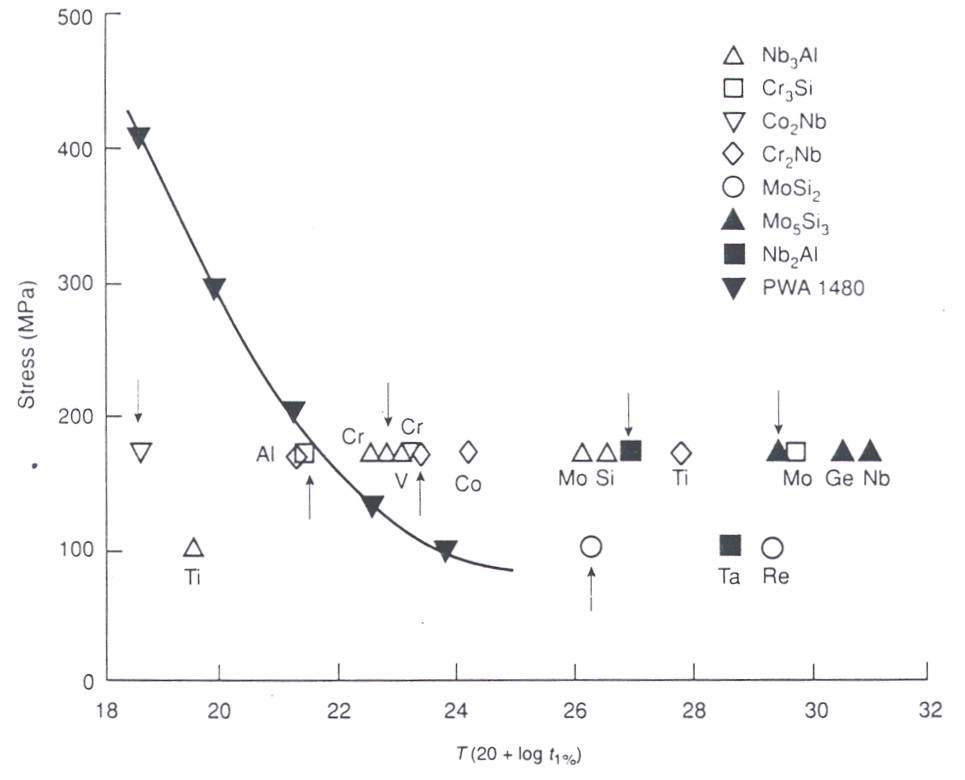
\includegraphics[width=12cm]{LMplotforintermetallics}
\caption{Larson-Miller plot of the stress for 1\% creep in steady state, comparing creep resistances of intermetallic compounds and their alloys against a single crystal superalloy, PWA 1480 ~\cite{anton89, anton89b, shah95}.}
\label{fig:LMplotforintermetallics}
\end{center}
\end{figure}
%
%
\begin{figure}[H]
\begin{center}
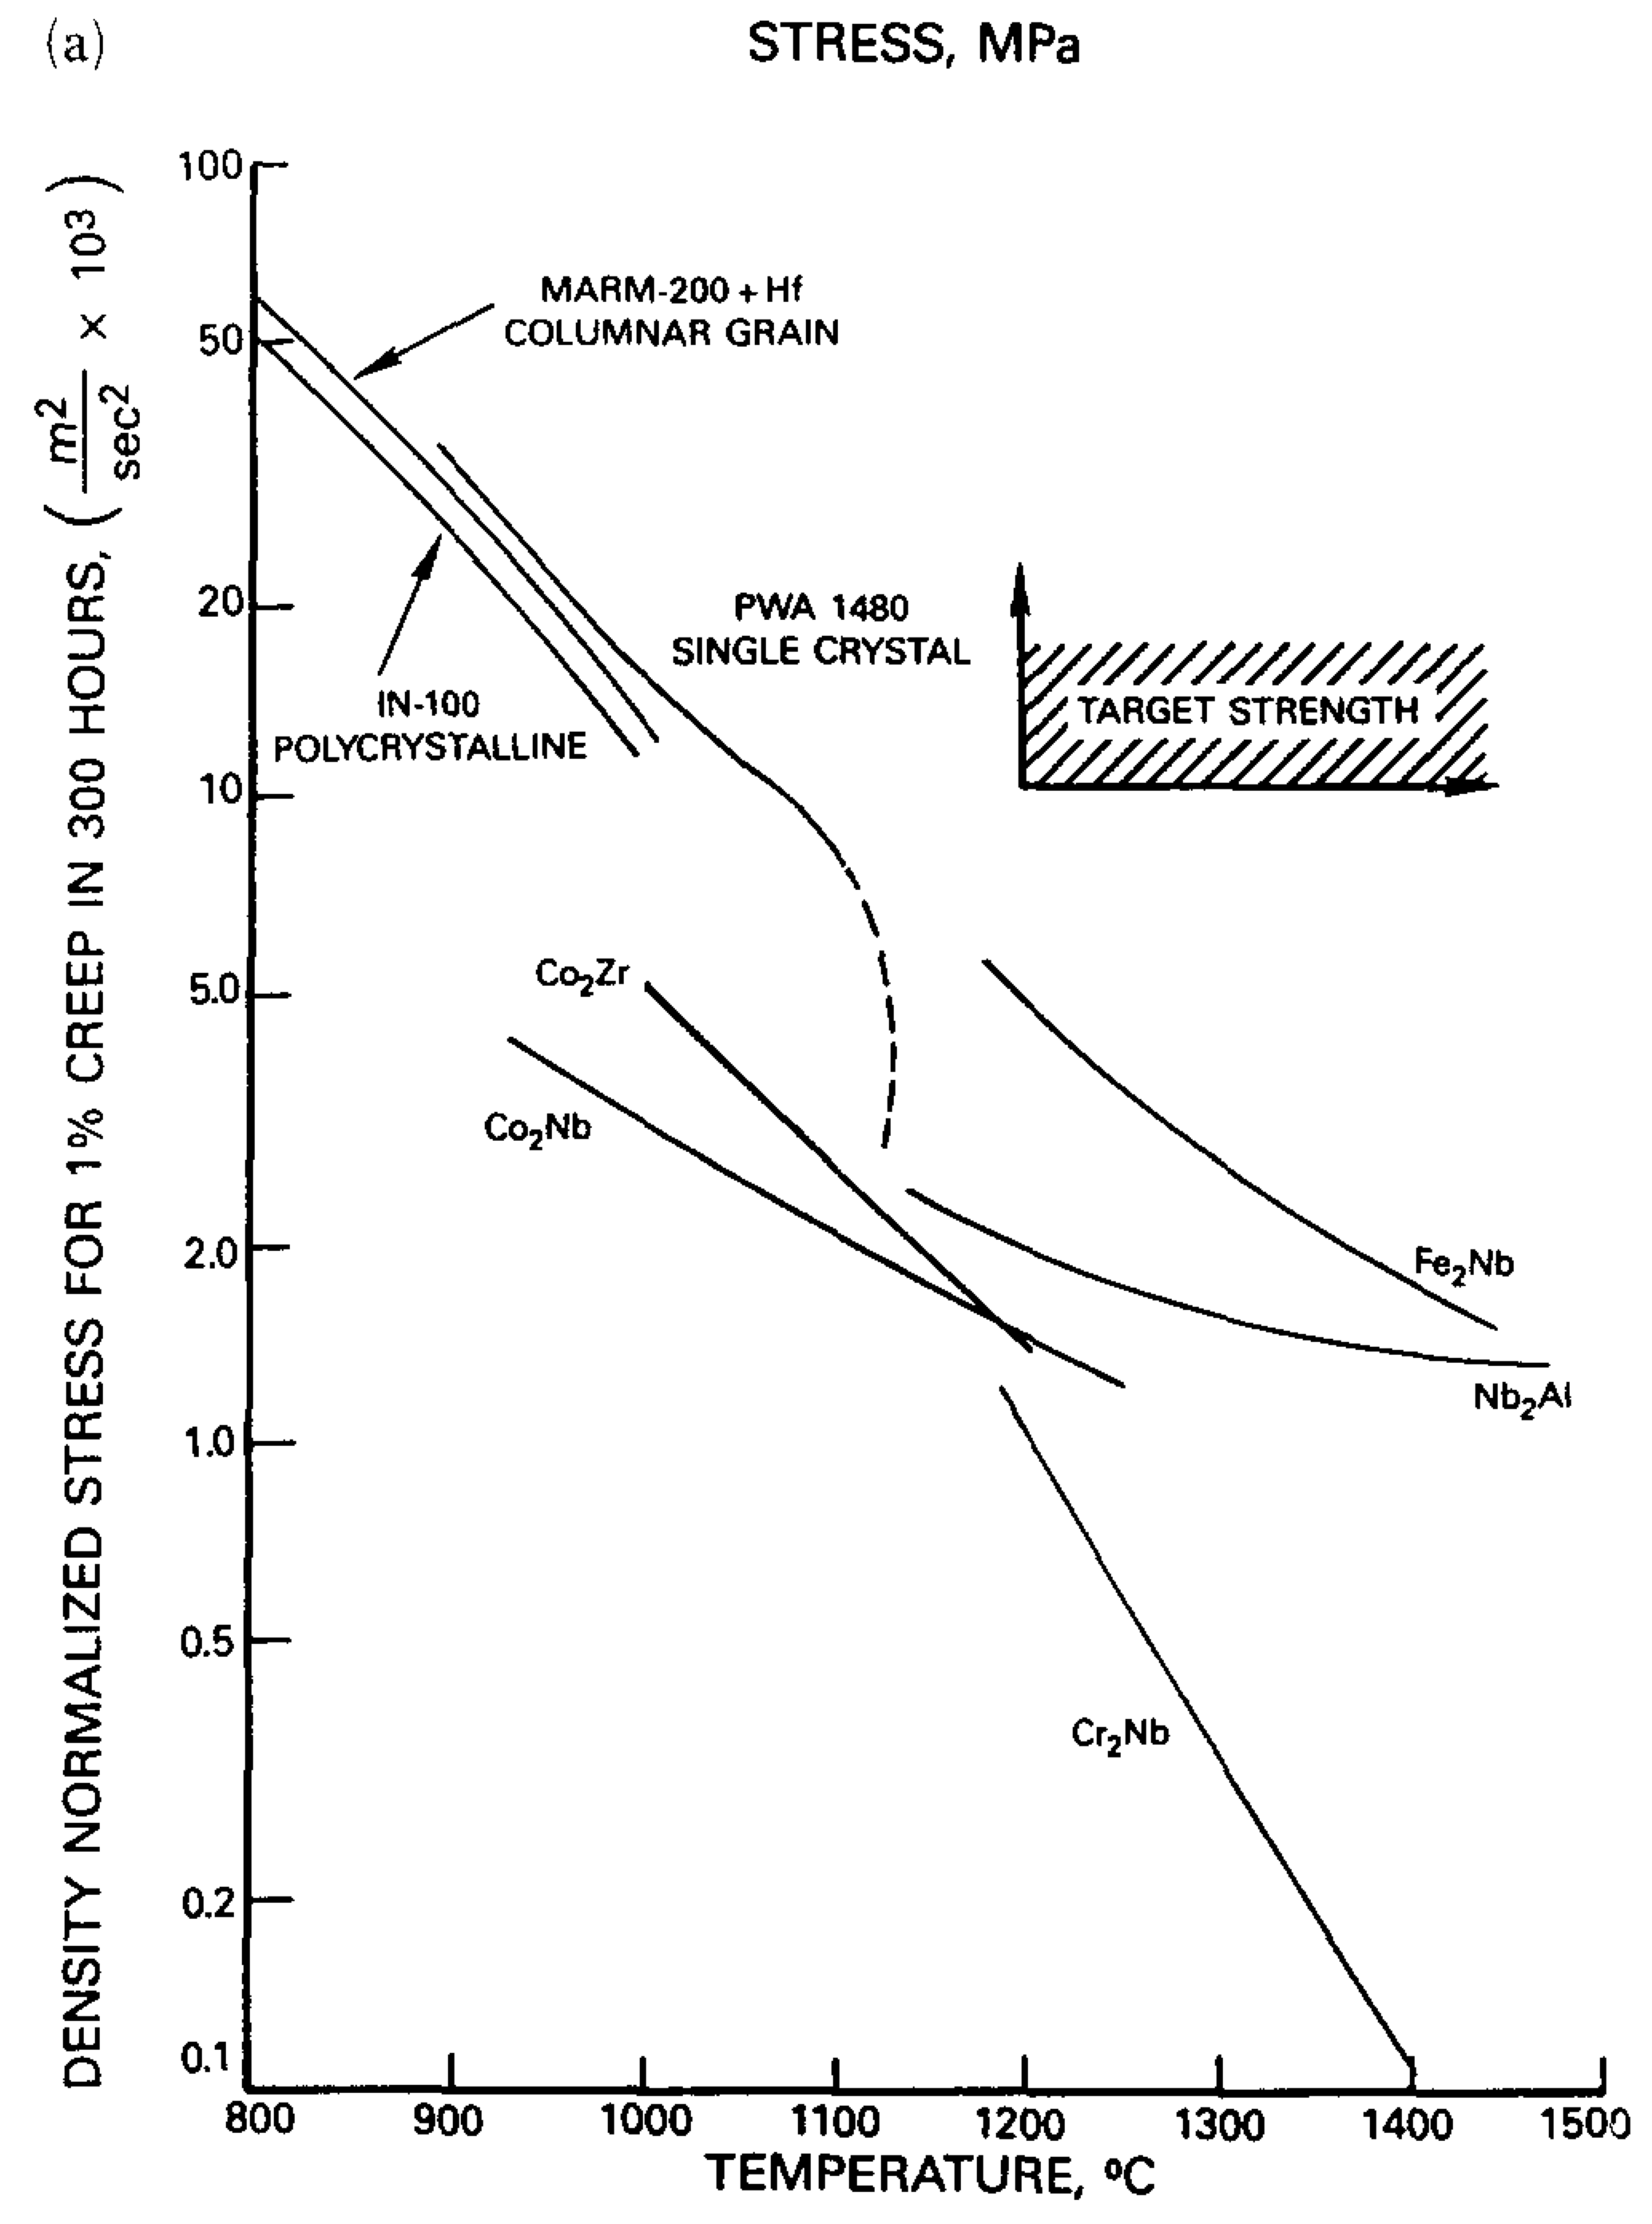
\includegraphics[width=10cm]{conbzr}
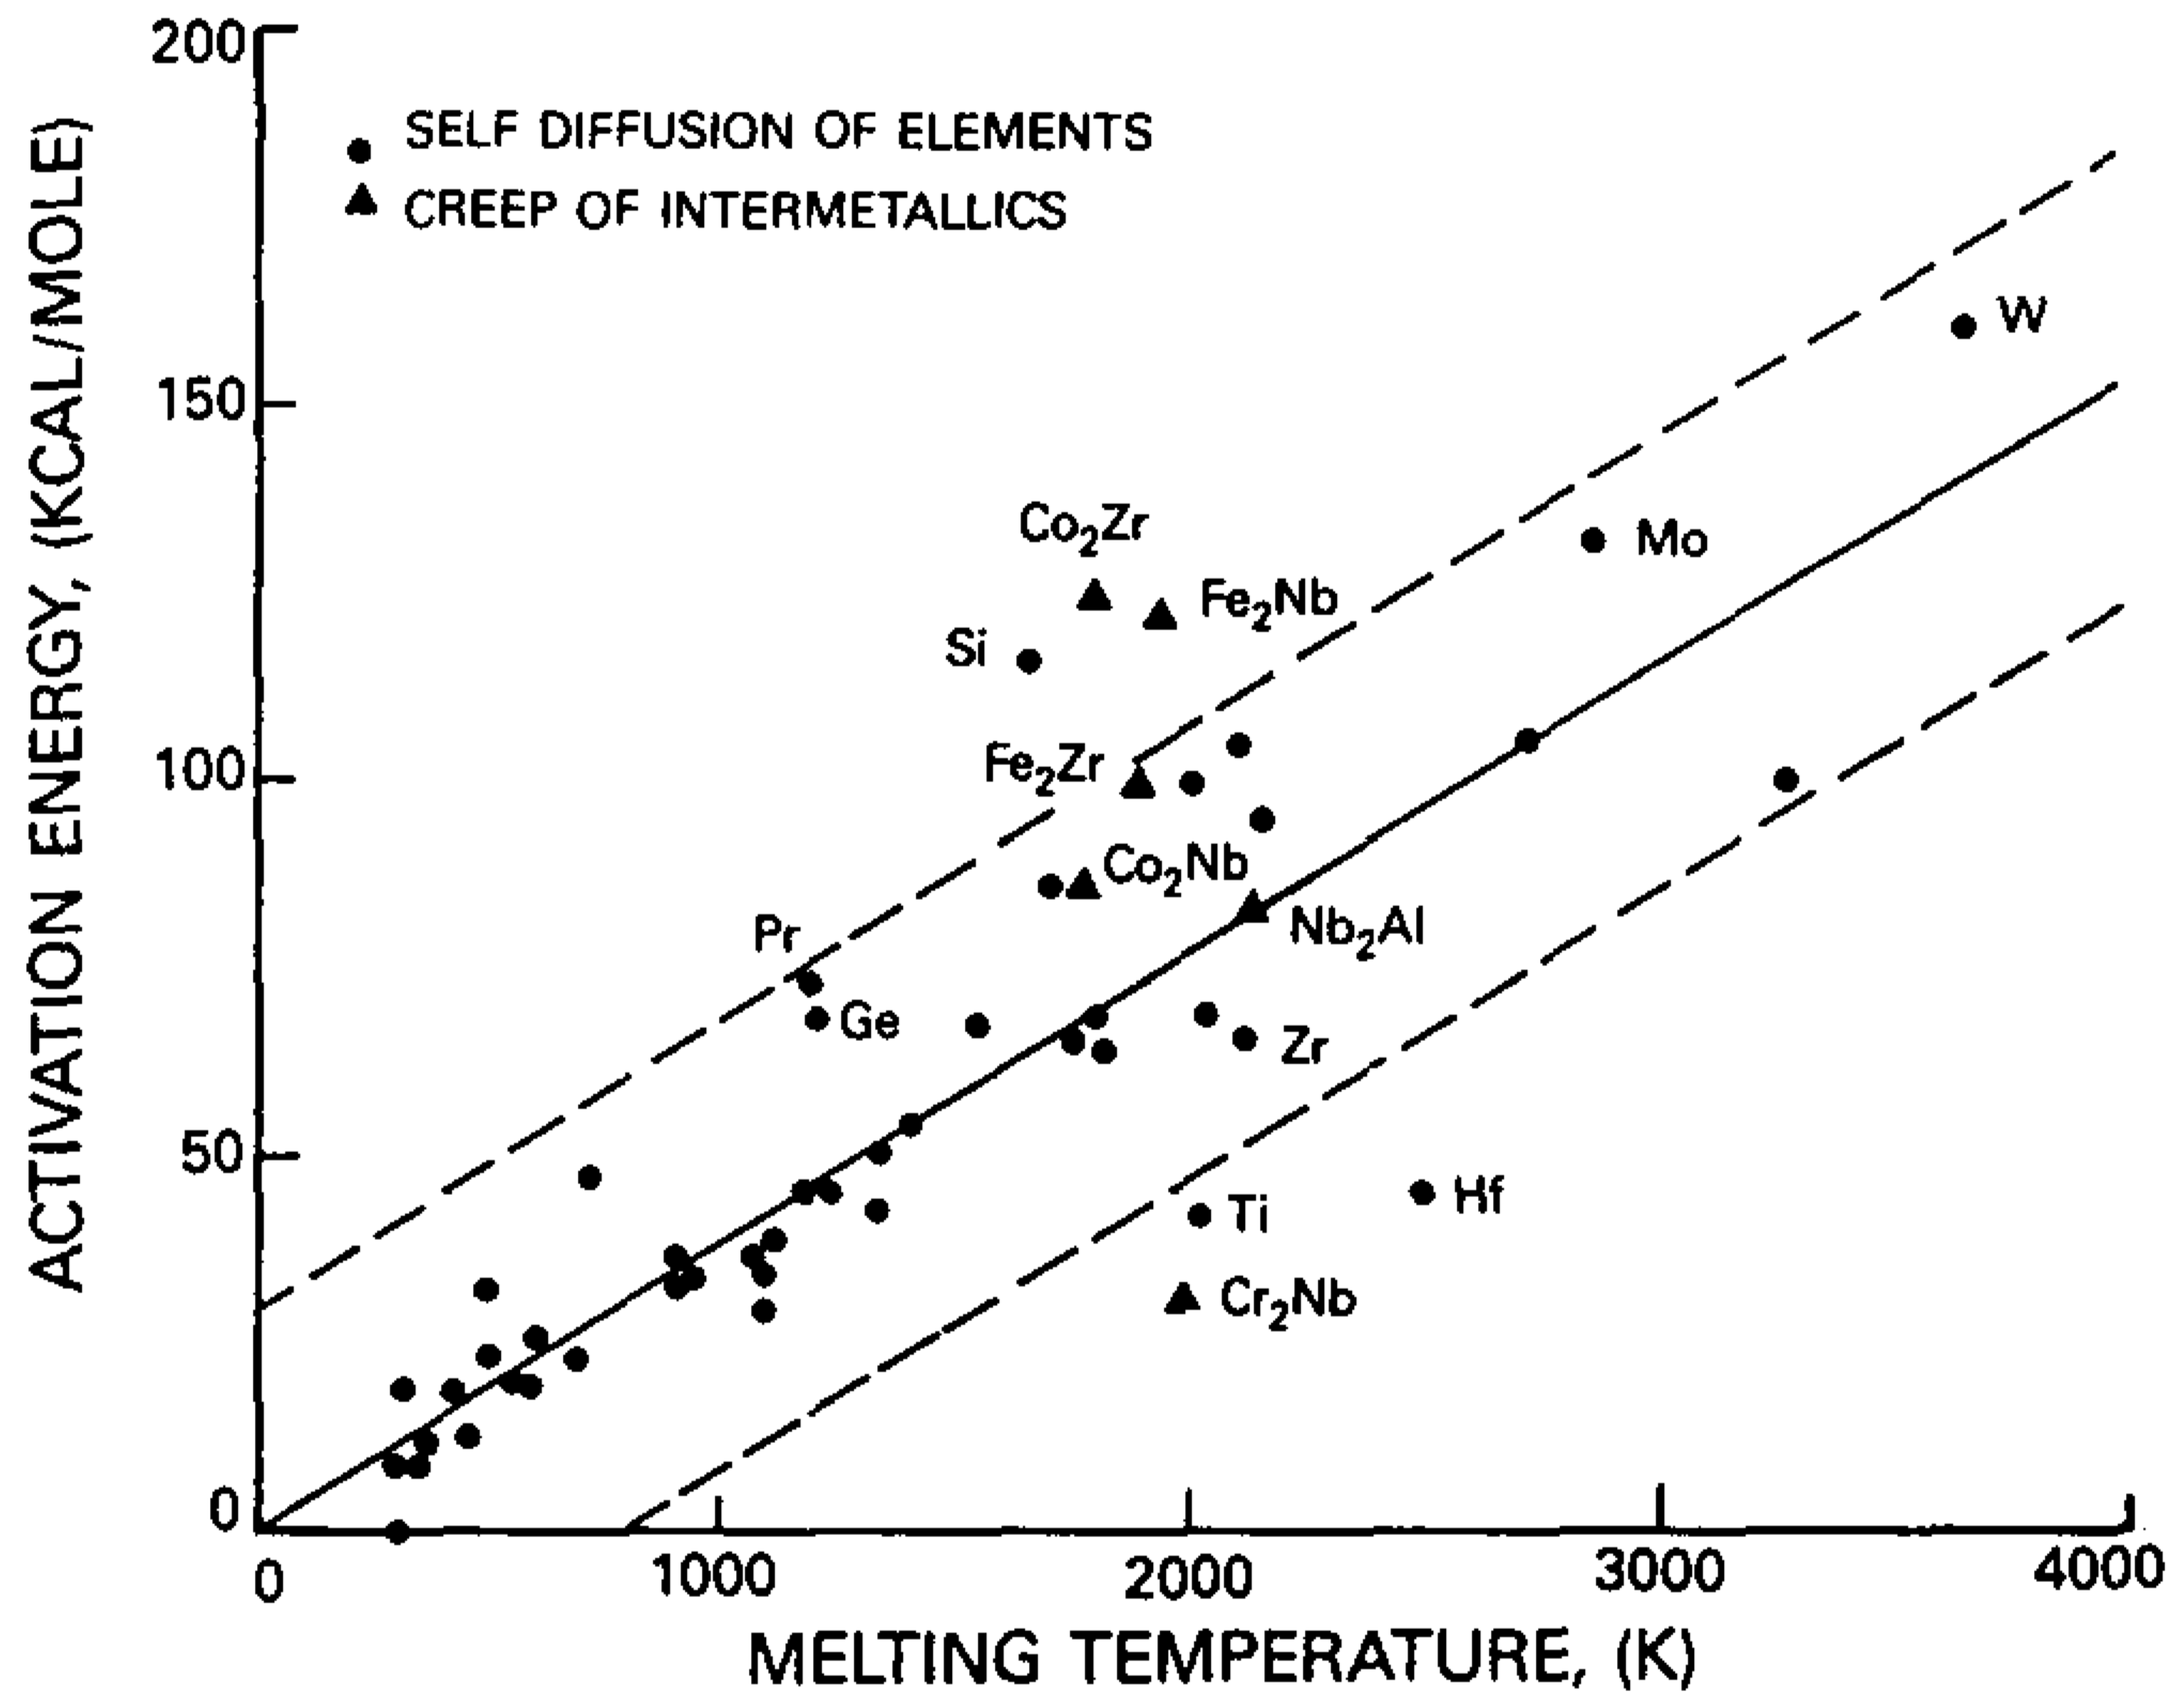
\includegraphics[width=10cm]{q}
\caption{(a) Density-normalised stress for 1\% creep in 300 hours for Co$_2$Zr, Co$_2$Nb, Fe$_2$Nb, Cr$_2$Nb and Nb$_2$Al, measured against several bench-mark poly-crystalline superalloys.  (b) Activation energy as a function of melting temperature for TCP intermetallics and relevant elements ~\cite{anton92}.}
\label{fig:conbzr}
\end{center}
\end{figure}
%


\section{Refractory Metal Silicide Systems}

In the last decade, the academic community has given molybdenum and niobium silicides the most attention.  Although they out-perform nickel-base superalloys in high-temperature creep, they form non-protective oxides at intermediate temperature ~\cite{ miracle94b, mitra06, ochiai06, sauthoff88, yanagihara96}.  Alloying can improve their oxidation resistance ~\cite{ramberg93, tomasi97, raj95a}, but can result in a decrease in high-temperature mechanical properties.

Low ambient temperature fracture-toughness is a common thread that runs through data on silicides explored for high-temperature applications  ~\cite{kumar94, miracle94b, shah92, sadananda99}.

Preliminary results show silicides with unoptimised microstructures containing micro-cracks display creep properties with a 200\celsius\ increase in temperature capability over nickel-base superalloys (Figures \ref{fig:creepshah92_1} and \ref{fig:creepshah92_2}).  However, these silicides have not been designed to contain a toughening phase and are very brittle, possessing poor fracture-toughness at room temperature.  Research thus far on molybdenum silicides and borosilicides, together with silicides of niobium, chromium, vanadium, titanium, tantalum and tungsten, will be described. 
%
\begin{figure}[H]
\begin{center}
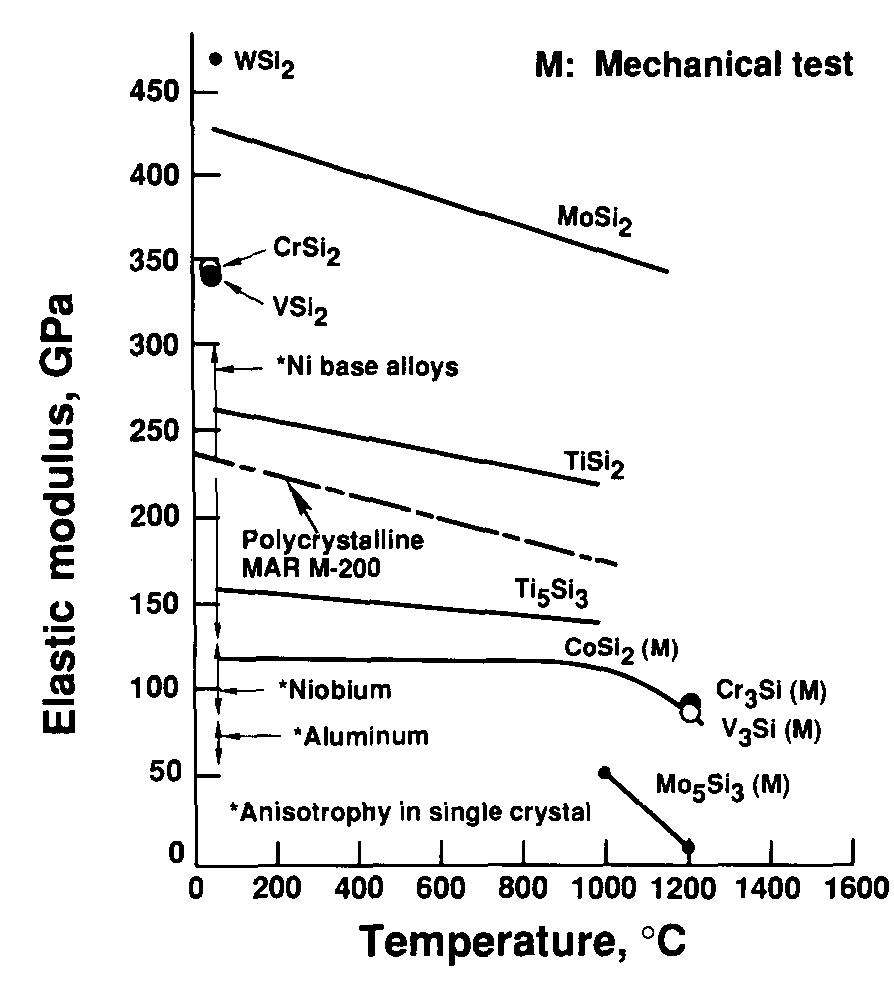
\includegraphics[width=.75\textwidth]{creepshah92_1}
\vspace{-.3cm}
\caption{Measured elastic modulii of silicide systems and nickel-base superalloys between room temperature and 1200\celsius ~\cite{shah92}.}\label{fig:creepshah92_1}
\end{center}
\end{figure}
\vspace{-.5cm}
%
\begin{figure}[H]
\begin{center}
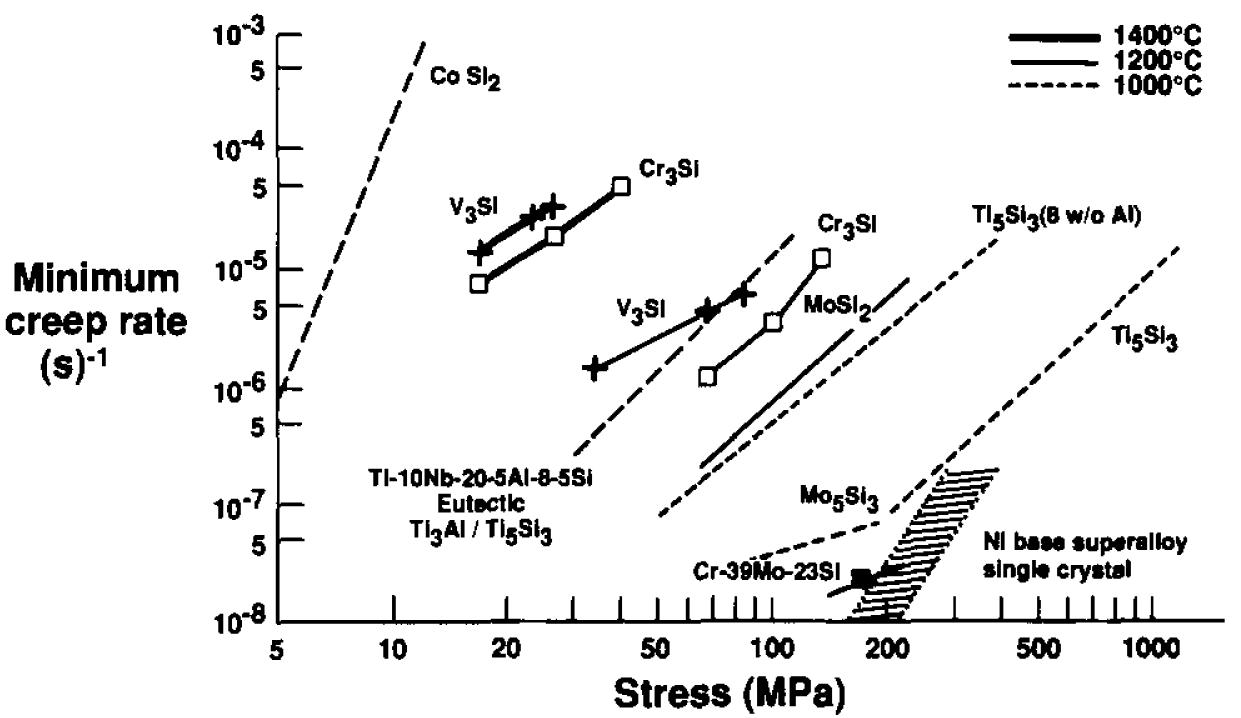
\includegraphics[width=.99\textwidth]{creepshah92_2}
\caption{Comparison of minimum compressive creep-rate of silicides and nickel superalloys vs stress between 1000--1400\celsius\ ~\cite{shah92}.}\label{fig:creepshah92_2}
\end{center}
\end{figure}
%



%
 			
\subsection{Molybdenum Silicides}\label{subsection:MoSis}

Molybdenum silicides have been heavily researched as they have high melting points of above 2000\celsius\ ~\cite{svechnikov70}, high-temperature strength-retention, and can possess good high-temperature oxidation resistance ~\cite{brady00, mitra06, raj95a,  ochiai06}.  However, they are susceptible to ``pesting" ~\cite{inui00, ochiai06, shah92, yanagihara96}.  This can be observed for MoSi$_2$ in the graph of mass change versus time in Figure \ref{fig:MoSi2_oxidation}.  At 500\celsius, MoSi$_2$ gains over 6\milli \gram\usk\centi\rpcubic\meter\ linearly.  In comparison, nickel-based superalloys gain substantially less than 1\milli \gram\usk\centi\rpcubic\meter\ in a parabolic fashion.  MoSi$_2$, despite being the molydenum silicide with the highest Si content, is unable to form a protective silica layer to prevent pesting.  Hot isostatic press (HIP) manufactured powder specimens fare better than cast specimens.  The smaller grains in HIP manufactured powder specimens allow for the short-circuit diffusion of Si through grain-boundaries to the oxidation zone.  This allows the specimens to form more protective silica-rich oxides; nonetheless, their oxidation rates are still linear.

There are three molybdenum silicides in the Mo--Si binary: Mo$_3$Si, Mo$_5$Si$_3$ and MoSi$_2$ (Figure: \ref{fig:MoSi}) ~\cite{svechnikov70}.  Molybdenum melts at 2620\celsius\ and has a density of 10.28  \gram\usk\centi\rpcubic\meter.  Mo$_3$Si has a density of 8.4  \gram\usk\centi\rpcubic\meter.  It undergoes a peritectic reaction at 2023\celsius.  This is very close to the eutectic temperature of MoSi$_3$ and Mo$_5$Si$_3$ at 2020\celsius.  Mo$_5$Si$_3$ melts at 2180\celsius, and has a lower density.  It forms a eutectic with MoSi$_2$ at 1900\celsius.  Molybdenum silicide alloys that do not contain molybdenum solid-solution can be slightly less dense nickel-based superalloys.  Alloys that contain Mo solid-solution tend to be heavier than superalloys; of course, this is dependent on phase fraction.
%
\vspace{6mm}
\begin{figure}[H]
\begin{center}
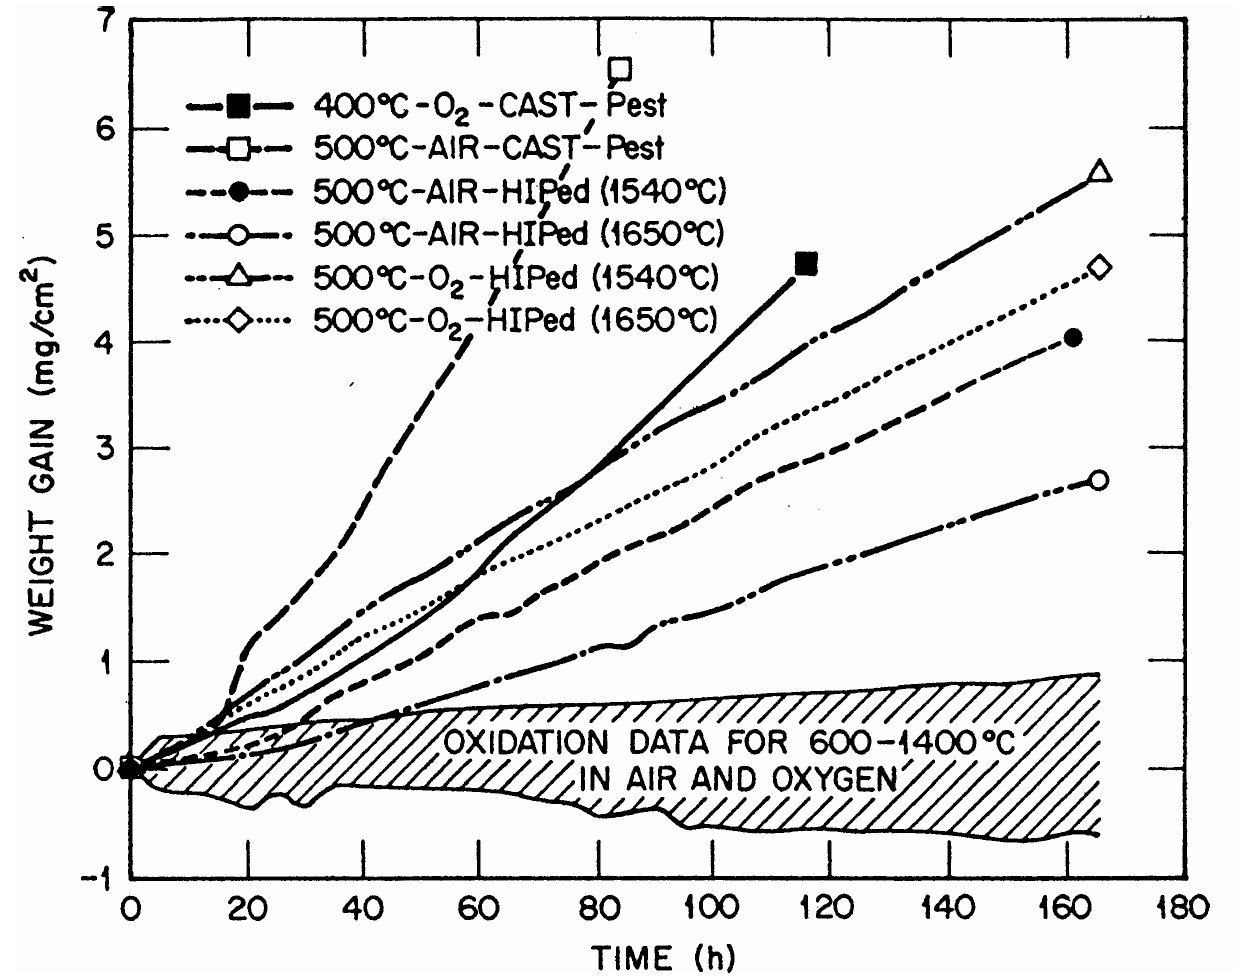
\includegraphics[width=11cm]{MoSi2_oxidation}
\caption{Mass change of MoSi$_2$ specimens, manufactured by either hot isostatic press (HIP) manufacture or casting, during oxidation at temperatures between 400--1400\celsius\ ~\cite{inui00}.}
\label{fig:MoSi2_oxidation}
\end{center}
\end{figure}
\vspace{-5mm}
%


%
\vspace{6mm}
\begin{figure}[H]
\begin{center}
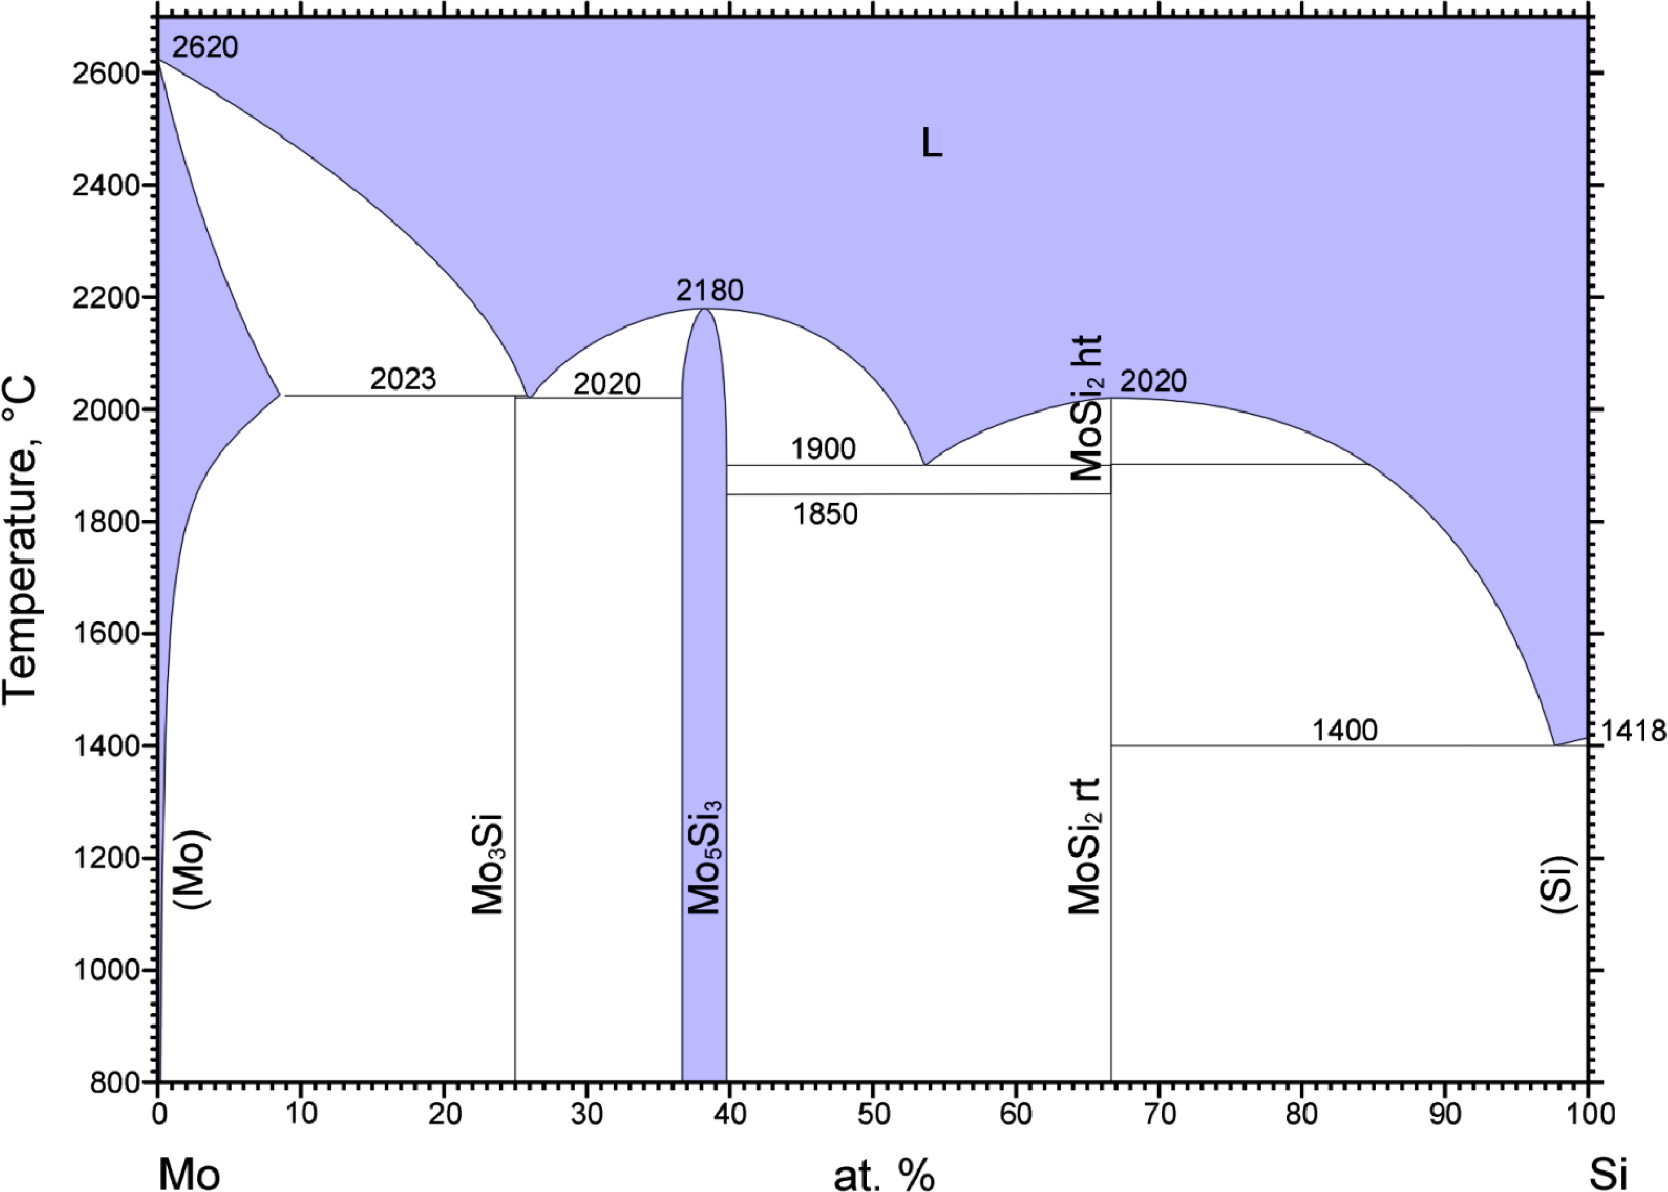
\includegraphics[width=15cm]{MoSi}
\caption{The Mo-Si binary phase-diagram ~\cite{svechnikov70}}
\label{fig:MoSi}
\end{center}
\end{figure}
%

\clearpage
Mo$_3$Si is attractive as it can be in equlibrium with the ductilising solid-solution phase. The structural properties have been evaluated ~\cite{rosales00, swadener01}.  It has a low fracture-toughness of 3 \mega\pascal\m$^{\frac{1}{2}}$.  Its compressive strength at 1400\celsius\ was found to decrease with increasing Si content and decreasing strain-rate.  At 10$^{-3}$/s, Mo$_3$Si shows a yield strength of 660 \mega\pascal\ at a Si content of 22at.\%, and a yield strength of 300 \mega\pascal at a Si content of 25at.\%.   Mo$_3$Si has inferior yield strength to Mo$_5$Si$_3$.  Using atomic force microscopy, <100>\{010\} slip was observed in nano-indentation samples oriented in <100>, <110> or <111> orientations.  <100> was found to be the orientation with the highest indentation modulus ~\cite{swadener01}.

Mo$_5$Si$_3$ has been quite heavily researched because of its excellent high-temperature mechanical properties (Figure \ref{fig:LMplotforintermetallics}).  It has the highest melting point in the Mo--Si binary ~\cite{svechnikov70}.  The high-temperature structural performance of Mo$_5$Si$_3$ is related to its high-thermal stability and the existence of mixed metallic and covalent bonding within its crystal structure ~\cite{sakidja08}.  This structural performance is not confined only to the 5:3 molybdenum silicide; 5:3 silicides of Nb and Ti Mo$_5$Si$_3$ has poor room temperature fracture-toughness of 3  \mega\pascal\m$^{\frac{1}{2}}$\ and poor oxidation properties at intermediate and high-temperatures ~\cite{akinc99, anton89, anton89b}.  This is below the fracture-toughness threshold that would allow for specimen machining.  The inclusion of molybdenum solid-solution to provide a degree of plastic deformation decreases high-temperature performance, increases density and contributes to poorer oxidation behaviour.  

MoSi$_2$ has the best high-temperature oxidation resistance out of the molybdenum silicides due to its Si content.  Its susceptibility to pesting, as seen in Figure \ref{fig:MoSi2_oxidation}, can be mitigated by subjecting specimens to a pre-treatment at a high-temperature and low oxygen partial pressure to allow Si to form a protective silica layer.  No solution has yet been found for its poor fracture-toughness ~\cite{anton89, kishida10, shah95, shah92}.  Attempts at incorporating ductile solid-solution composing of W, Nb and Mo were met with failure ~\cite{dimiduk03}.  Interfacial interactions led to gross microstructural destabilisation.  Current consensus is that there is no feasible way to design MoSi$_2$-based alloys with sufficient creep, fracture and oxidation properties that would render them suitable for high-temperature structural applications ~\cite{dimiduk03, sekido07}.

Akinc has reported that 3 at.\% boron additions to Mo$_5$Si$_3$ improves its oxidation properties between 800 -- 1500\celsius\ by as much as 5 orders of magnitude (Figure \ref{fig:Mo5Si3_oxidation}).  During the initial onset of oxidation, a boro-silicate glass forms in competition with MoO$_3$.  MoO$_3$ is the cause of catastrophic oxidation of Mo$_5$Si$_3$; it sublimes at 750\celsius\ ~\cite{brewer90} and is non-protective.  The boro-silicate glass experiences viscous flow at 1000\celsius\ and promotes closure of sub-micron scale porosity left behind due to MoO$_3$ volatilisation; thus minimising subsequent oxidation of Mo into MoO$_3$ (Figure \ref{fig:MoSi_oxidationpictures}) ~\cite{akinc99}.  This is one reason why the scientific community believe that it is worthwhile to explore the Mo--Si--B system as an alloy design space for ultra-high-temperature applications. 


% 
\begin{figure}[H]
\begin{center}
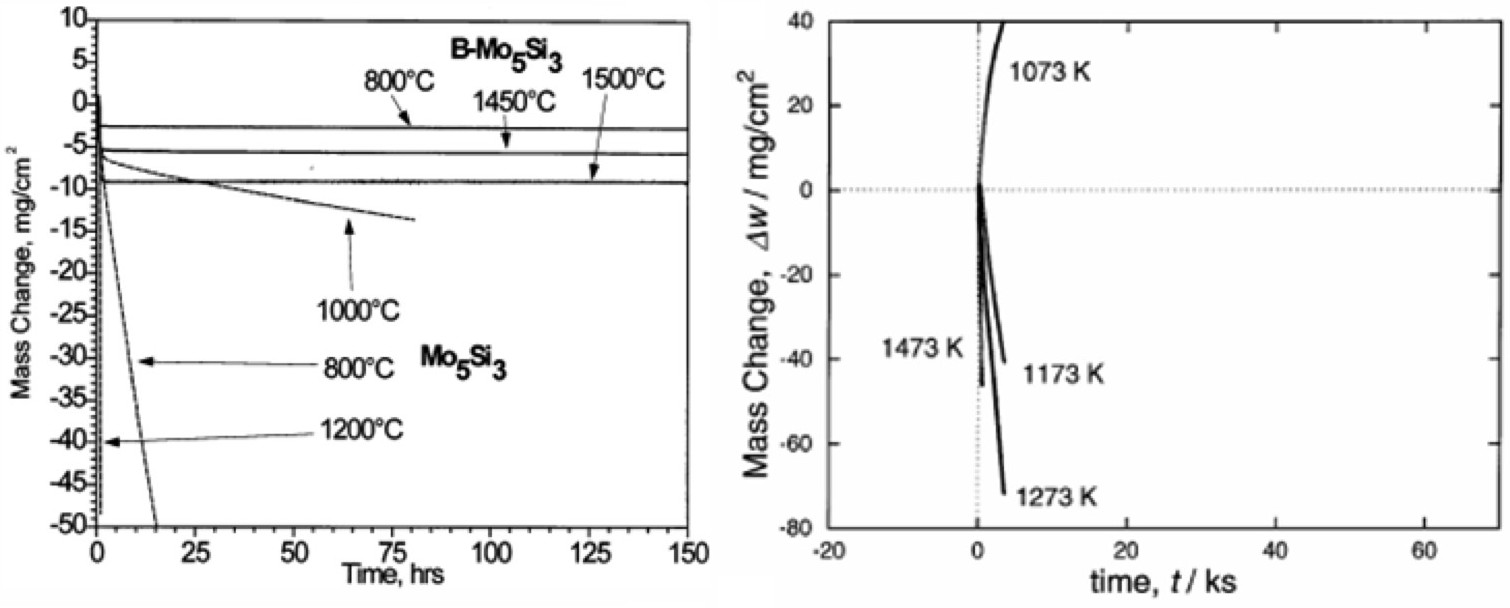
\includegraphics[width=.95\textwidth]{Mo5Si3_oxidation}
\vspace{-.3cm}
\caption{Mass change of Mo$_5$Si$_3$ during oxidation at temperatures between 800--1500\celsius\ ~\cite{akinc99}.}\label{fig:Mo5Si3_oxidation}
\end{center}
\end{figure}
\vspace{-.5cm}
%
\begin{figure}[H]
\begin{center}
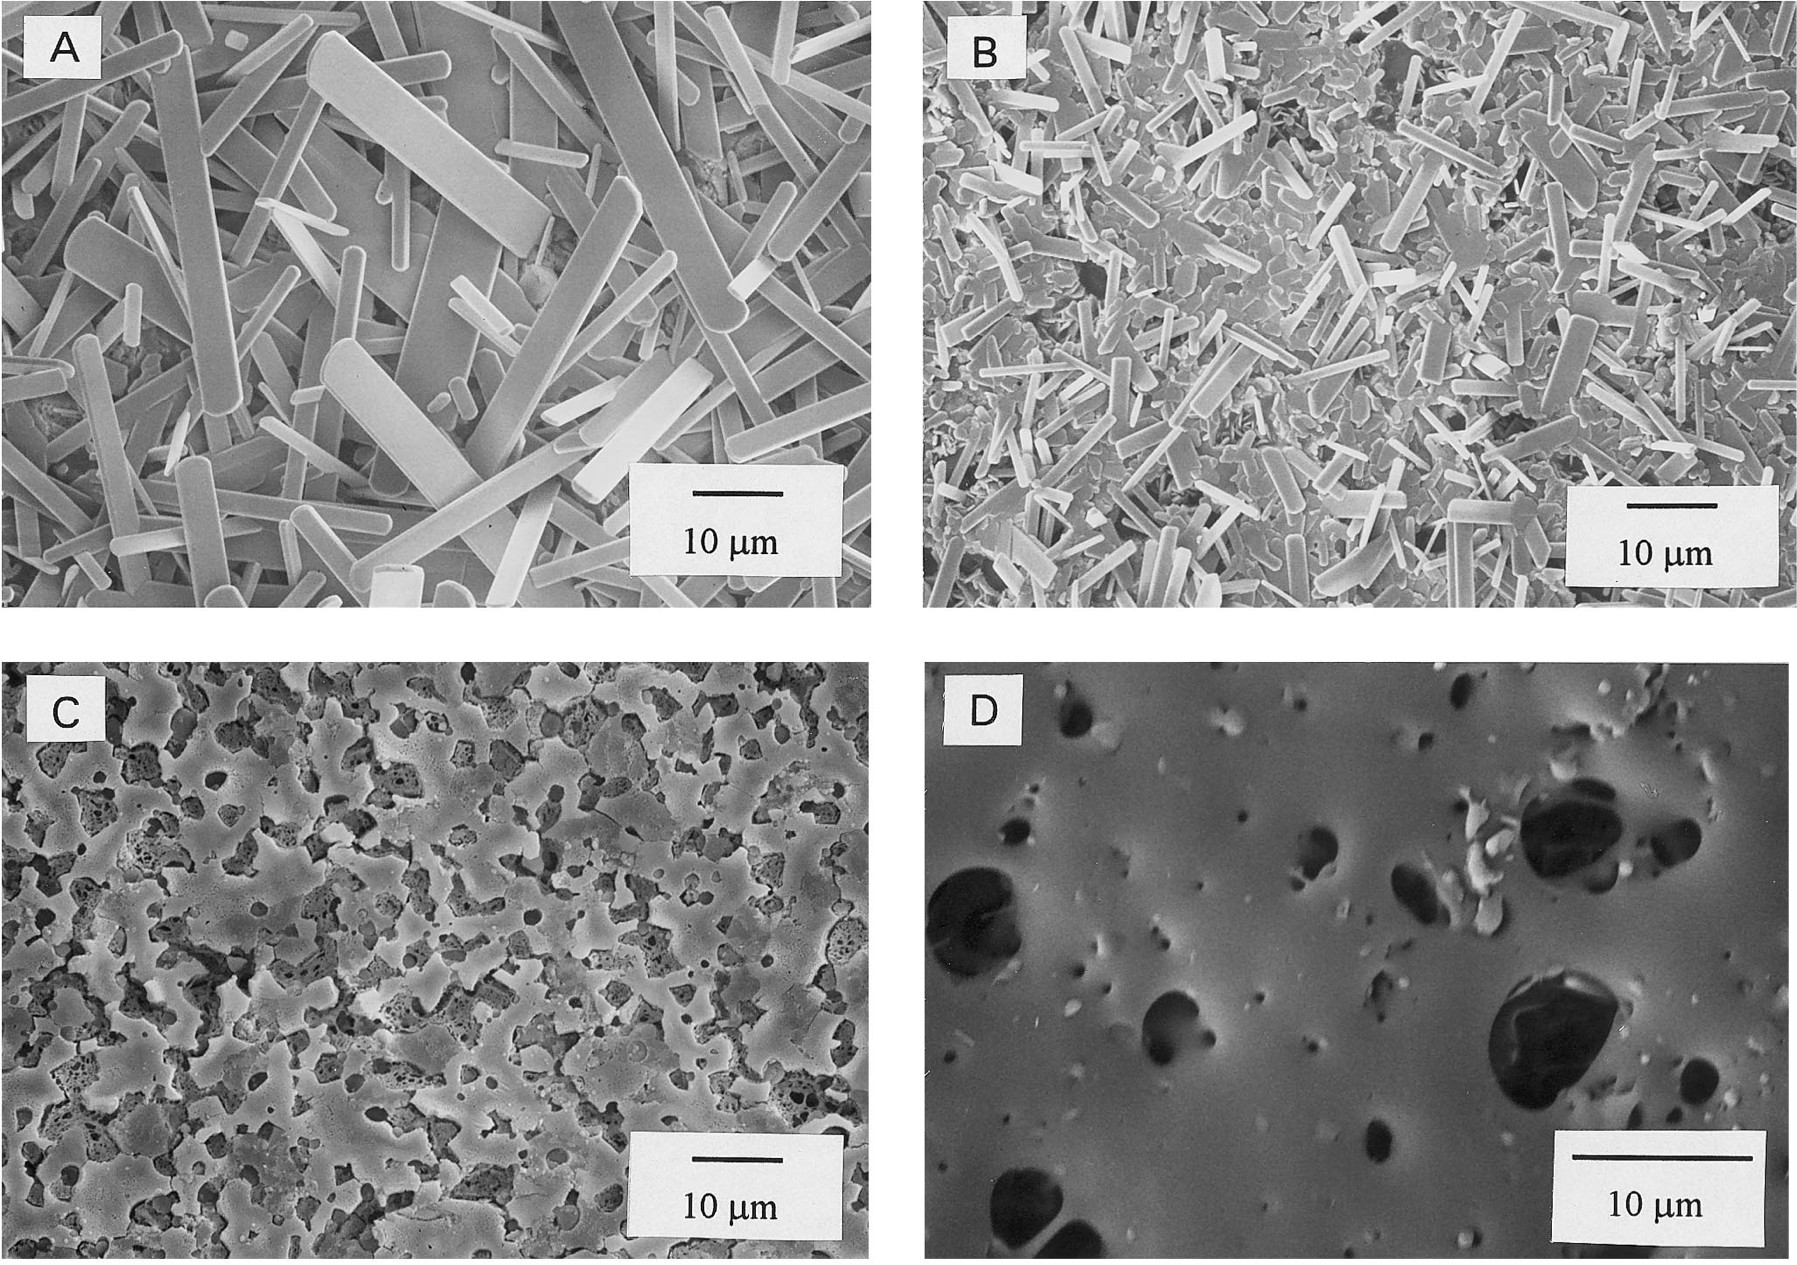
\includegraphics[width=.9\textwidth]{MoSi_oxidationpictures}
\vspace{-2mm}
\caption{SEM micrographs showing the transition of the initial oxide from MoO$_3$ to a boro-silicate glass ~\cite{akinc99}.}
\label{fig:MoSi_oxidationpictures}
\end{center}
\end{figure}
\vspace{-1cm}
%

\subsubsection{Molybdenum Borosilicide Alloys}

The Mo$_5$SiB$_2$ phase has been a focus of great interest to the high-temperature materials community due to its unparallelled creep properties at 1500\celsius\ ~\cite{hayashi04, ito01}.  This is a 400\celsius\ increase in creep capability over nickel superalloys.  At 1300\celsius, its creep-rate is about 3 orders of magnitude lower than a well-oriented MoSi$_2$ sample.  It is a boro-silicide variant of Mo$_5$Si$_3$.

The T$_2$ phase is a layered D8$_1$ crystal structure with a very high packing density (Figure \ref{fig:T2structure}) ~\cite{rawn01, sakidja08}.  The `A' and `A$_{\frac{1}{2}\frac{1}{2}}$' layers of pure Mo are sandwiched between layers of alternating Mo+Si and Mo+B layers.  At first glance, the layered structure could result in poor properties in shear, akin to that in graphite, but this has not been found to be the case.  The very large unit cell contains 20 Mo atoms, 4 Si atoms and 8 B atoms.  The large difference in atomic radii between Si and B ``neccessitates stacking arrangements" of the Mo layers such that distinct layers can be accommodated for Si and B.  

 
%
\vspace{8mm}
\begin{figure}[H]
\begin{center}
\includegraphics[width=9.5cm]{t2structure}
\caption{The crystal structure of Mo$_5$SiB$_2$ ~\cite{sakidja08}. }
\label{fig:T2structure}
\end{center}
\end{figure}
\vspace{-.2cm}
%
%
\begin{figure}[H]
\begin{center}
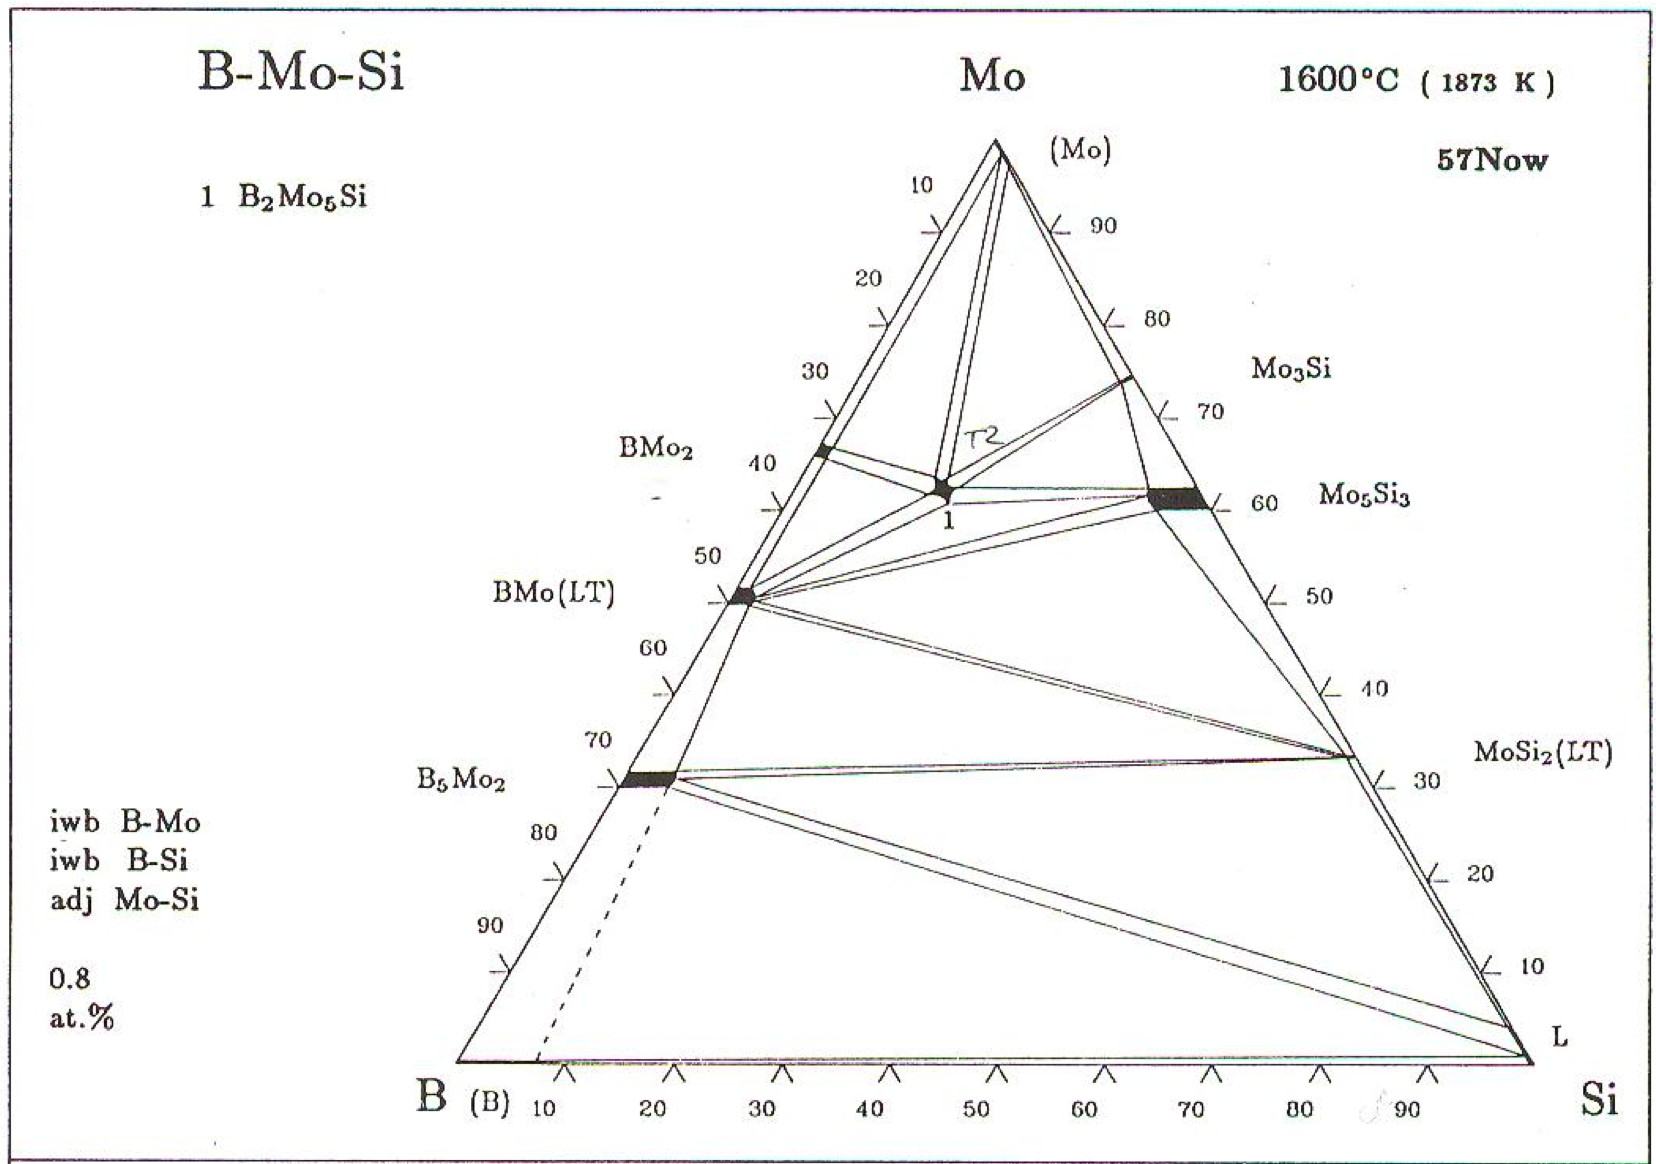
\includegraphics[width=\textwidth]{MoSiB_1600}
\caption{The ternary phase-diagram of Mo--Si--B ~\cite{nowotny57}.}
\label{fig:MoSiB_1600}
\end{center}
\end{figure}
%
%
\begin{figure}[H]
\begin{center}
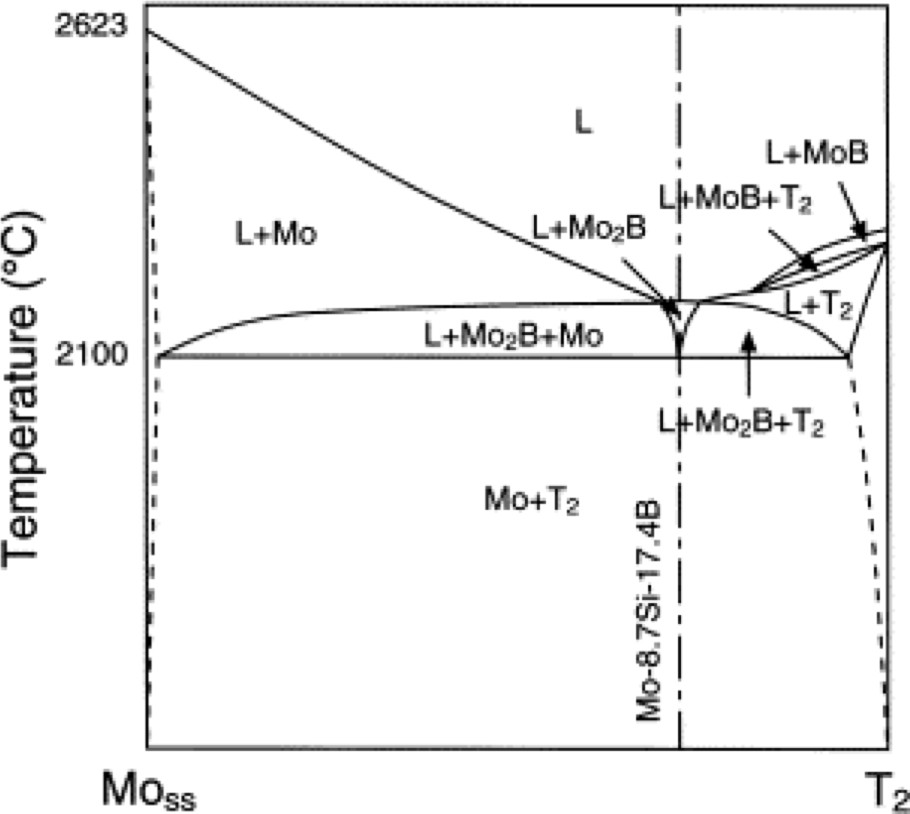
\includegraphics[width=8.5cm]{Mo-Mo5SiB2}
\caption{Mo--Mo$_5$SiB$_2$ pseudo-binary phase-diagram ~\cite{yoshimi03}.}
\label{fig:Mo-Mo5SiB2}
\end{center}
\end{figure}
%
\clearpage
Nowotny et al. identified the T$_2$ phase in a 1600\celsius\ isothermal section of the ternary in 1957 (Figure \ref{fig:MoSiB_1600})  ~\cite{nowotny57}.  A Mo--Mo$_5$SiB$_2$ pseudo-binary phase-diagram has also been constructed by Yoshimi et al. (Figure \ref{fig:Mo-Mo5SiB2}) ~\cite{yoshimi03}.    An alloy of T$_2$ particles in a solid-solution matrix, when subject to compression-creep at different temperatures and strain-rates, show a range of deformation behaviour ~\cite{alur04}.  Brittle fracture, plastic deformation and elastic deformation were all observed.  

Perepezko has explored the influence of microstructure control in the manufacture of Mo--Mo$_5$SiB$_2$ and Mo--Mo$_3$Si--Mo$_5$SiB$_2$ for ultra-high-temperature applications (Figure \ref{fig:Mo16Si8B}) ~\cite{perepezko01}.  The ternary eutectic is difficult to attain via casting because solidification segregation causes very stable borides and silicides to form instead.  Also, the liquidus-surfaces for Mo$_3$Si and T$_2$ around the ternary eutectic region are shallow (Figure \ref{fig:MoSiB_liquidus}).  The invariant eutectic can be by-passed during non-equilibrium solidification.  Mo$_3$Si and T$_2$ would form instead, and there will be very little toughening component in the microstructure (Figures \ref{fig:Mo16Si8B} and \ref{fig:MoSiB_witheutectic}).

Perepezko has introduced alloying elements such as Nb to stabilise the T$_2$ phase and destabilise boride reactions (Figure \ref{fig:MoSiB_withNb}) ~\cite{perepezko01, sakidja00}.  Nb can substitute for Mo to a large extent in solid-solution and T$_2$.  This increases microstructural control and allows for direct solidification of a two-phase solid-solution and T$_2$ alloy in the region shaded in the liquidus-projection (Figure \ref{fig:Mo19Nb12Si8B}). 

%
\begin{figure}[H]
\begin{center}
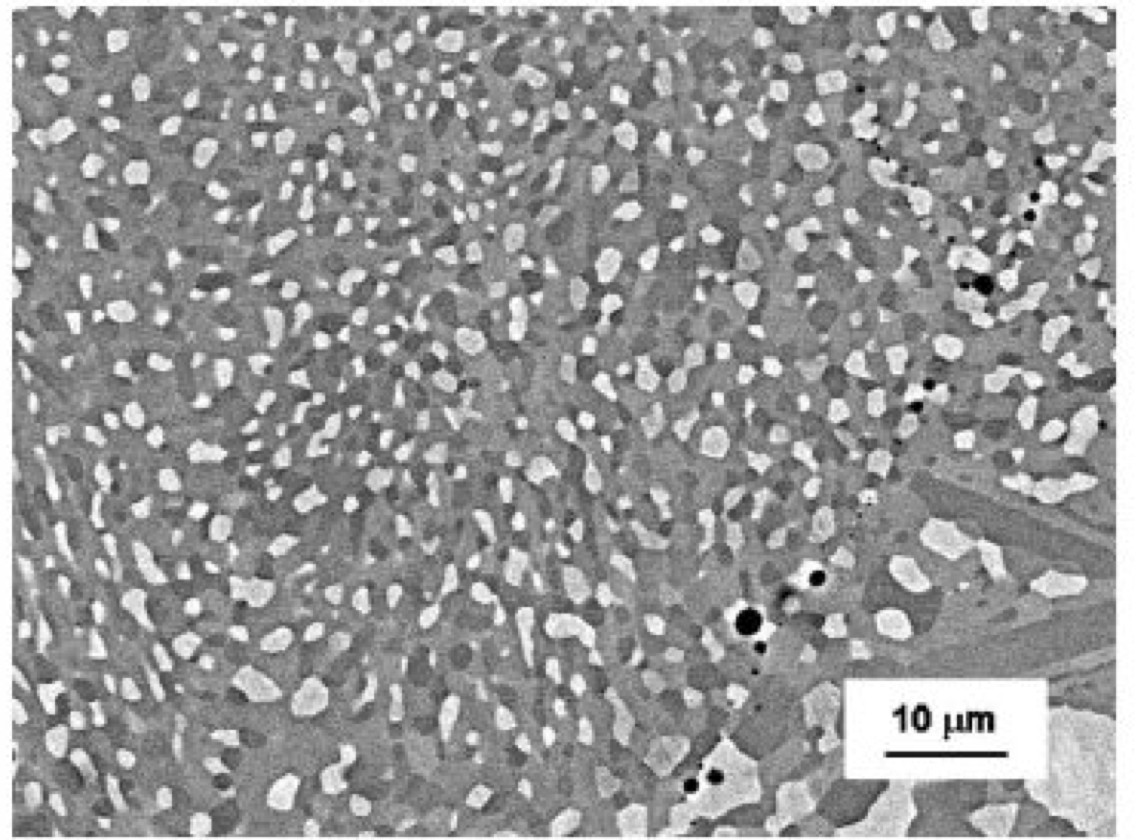
\includegraphics[width=11cm]{Mo16Si8B}
\caption{SEM micrograph of arc-melted Mo--16.8Si--8.4B ~\cite{perepezko01}.}
\label{fig:Mo16Si8B}
\end{center}
\end{figure}
%
%
\begin{figure}[H]
\begin{center}
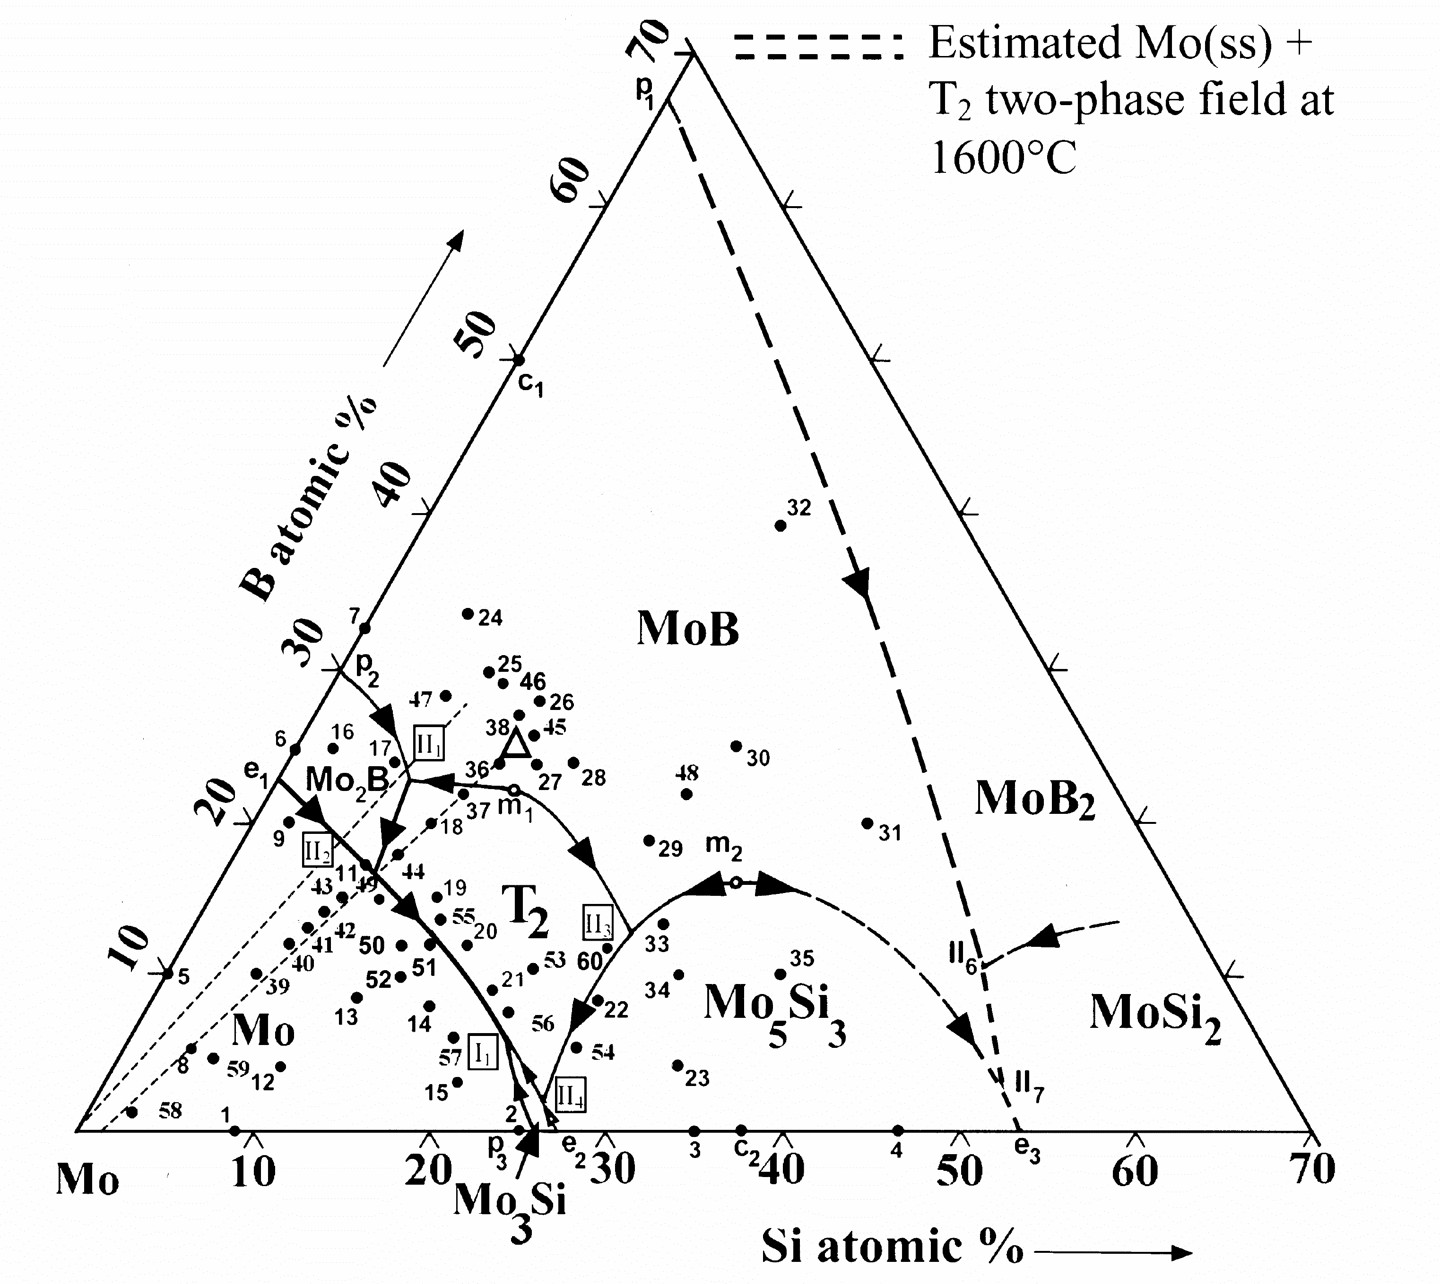
\includegraphics[width=14cm]{MoSiB_liquidus}
\vspace{-3mm}
\caption{The relevant portion of the Mo--Si--B liquidus projection T = 1873K ~\cite{perepezko01}.}\label{fig:MoSiB_liquidus}
\end{center}
\end{figure}
\vspace{-5mm} 	
%
%
\begin{figure}[H]
\begin{center}
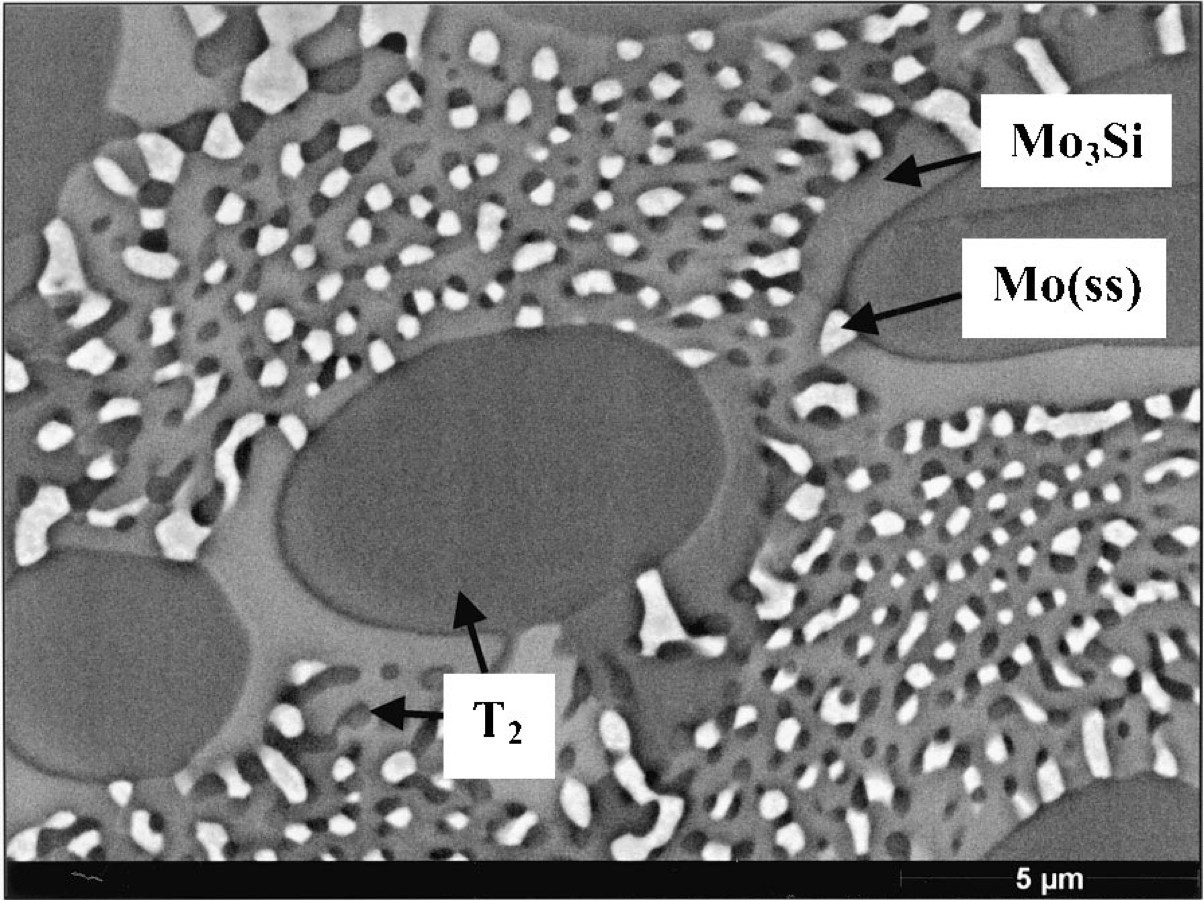
\includegraphics[width=10cm]{MoSiB_witheutectic}
\caption{Microstructure of an alloy with T$_2$ as the primary phase with a Mo(ss)--T$_2$--Mo$_3$Si invariant ternary eutectic ~\cite{perepezko01}.}
\label{fig:MoSiB_witheutectic}
\end{center}
\end{figure}
\vspace{.7cm} 
%
\begin{figure}[H]
\begin{center}
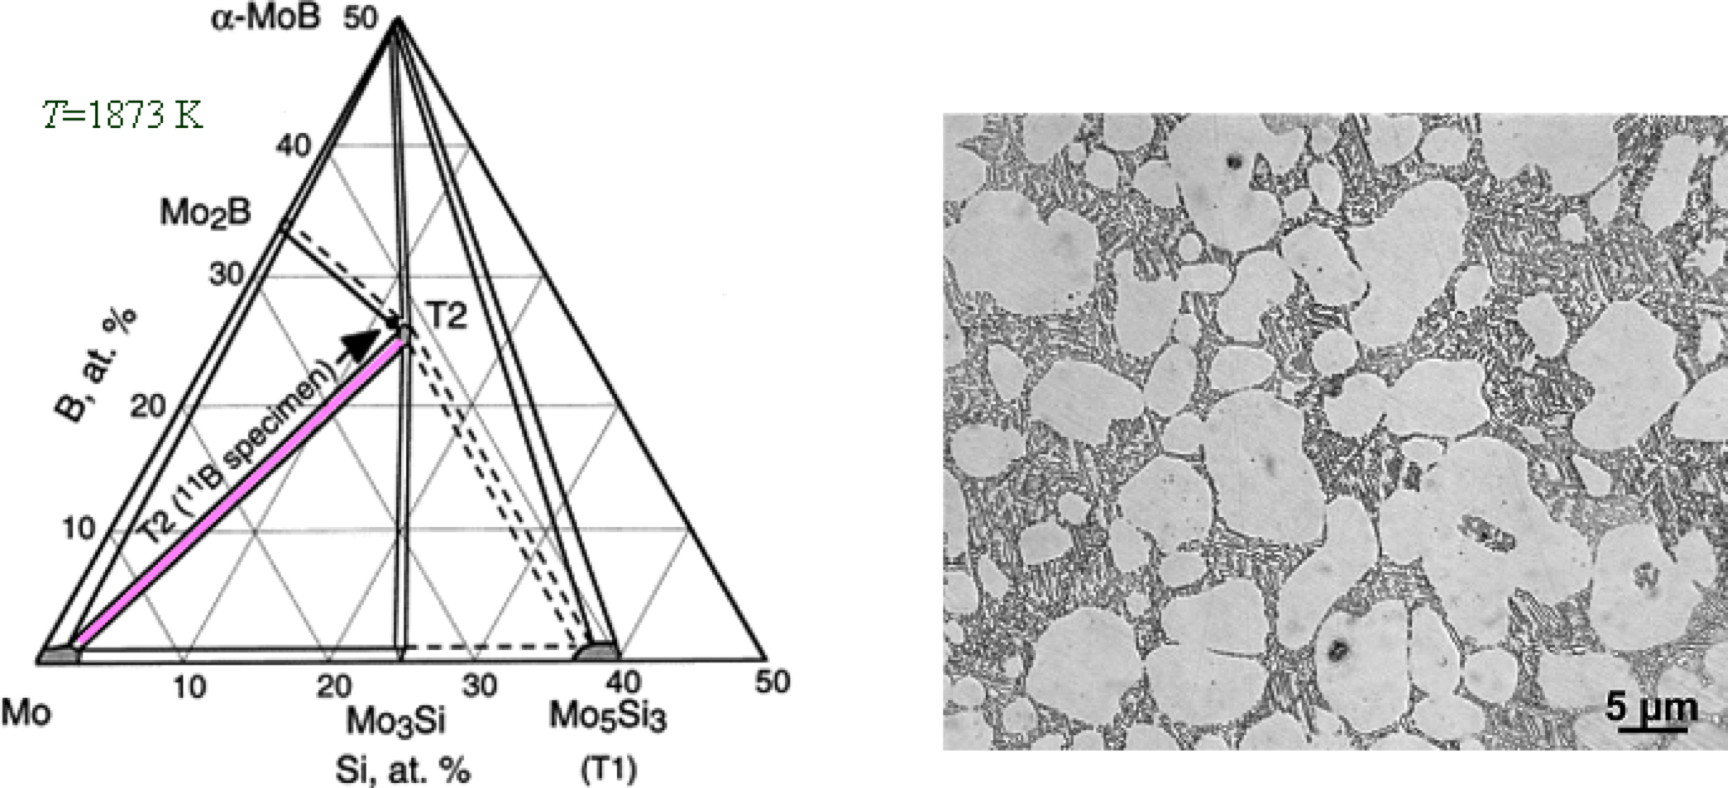
\includegraphics[width=\textwidth]{MoSiB_withNb}
\caption{Increase in solid-solution volume-fraction in the ternary eutectic with Nb-alloying ~\cite{perepezko01}.}\label{fig:MoSiB_withNb}
\end{center}
\end{figure}
%
\begin{figure}[H]
\begin{center}
\includegraphics[width=9cm]{Mo19Nb12Si8B}
\caption{SEM micrograph of a polished section of cast and annealed Mo--19.5Nb--12Si--8.5B (at.\%) ~\cite{perepezko01}.}\label{fig:Mo19Nb12Si8B}
\end{center}
\end{figure} 
%

The dislocations formed in annealed alloys containing Mo$_5$SiB$_2$ are mostly of edge character with Burgers vectors of <100], 1/2<111], and <110], implying either that screw dislocations are far more mobile then edge dislocations and/or that the dislocations observed are formed from condensation of vacancies.  It has been suggested ~\cite{sekido07} that these vacancies are formed in Mo-rich alloys of Mo$_5$SiB$_2$.  The edge dislocations that form when these vacancies aggregate act as heterogeneous nucleation sites for subsequent Mo precipitation.  In Mo-lean Mo$_5$SiB$_2$, defects that form do not contribute to dislocation formation ~\cite{sekido07}.

%
\begin{figure}[H]
\begin{center}
\includegraphics[width=16cm]{sekido07}
\caption{ Weak-beam dark-field images showing dislocations in Mo-rich T$_2$ phase.  The specimen was annealed for 20 hours at 1550\celsius.  The Burgers vector of the dislocations are (a) [010] and (b) [-1-10􏰇] ~\cite{sekido07}.}
\label{fig:sekido07}
\end{center}
\end{figure} 
%

A Mo--Si--B alloy was measured to have fracture-toughness values of 8 \mega\pascal\,m$^{\frac{1}{2}}$ at ambient temperature, to 25 \mega\pascal\,m$^{\frac{1}{2}}$ at 1400\celsius\ ~\cite{alur06}.  This is higher than the 3 \mega\pascal\,m$^{\frac{1}{2}}$ reported for molybdenum silicide alloys without a toughening solid-solution phase.  The dominant creep mechanisms in this alloy were found to be grain-boundary diffusion between 900--1200\celsius, and volume diffusion between 1200--1400\celsius.

In recent work ~\cite{kumar10}, the tensile creep properties of HIP-manfactured Mo--Si--B alloys have been successfully evaluated.  Tensile tests at a creep-rate of 10$^{-4}$s$^{-1}$ between 1000\celsius\ and 1200\celsius\ were performed on a solid-solution alloy, a solid-solution and ~35vol.\% T$_2$ alloy, and a solid-solution, T$_2$ and Mo$_3$Si alloy (Figure \ref{fig:ku10}).

%
\begin{figure}[H]
\begin{center}
\includegraphics[width=7.8cm]{ku10i}
\includegraphics[width=7.8cm]{ku10ii}
\vspace{5mm} 
\includegraphics[width=7.8cm]{ku10iii}
\caption{Tensile stress-strain curves from tests conducted at a nominal strain-rate of 10$^{-4}$ s$^{-1}$, at temperatures between 1000\celsius\ to 1200\celsius\ for (a) an Mo solid-solution alloy with <5vol.\% T$_2$ phase, (b) a two-phase alloy with solid-solution and T$_2$ phase (35 vol.\% ), (c) a three-phase alloy with solid-solution, T$_2$ and Mo$_3$Si ~\cite{kumar10}.}\label{fig:ku10}
\end{center}
\end{figure} 
%

In other recent work, this X$_5$SiB$_2$ phase has been described as a common 5:3 metal--metalloid compound that exists in many systems ~\cite{sakidja08}.  It is present in the Nb--Si--B ternary ~\cite{nunes97}, the V--Si--B ternary ~\cite{rodrigues09}, the Co--Si--B ternary, the Fe--Si--B ternary, the Mn--Si--B ternary, and the (Pt, Ir, Rh, Ru)--Si--B  ternaries ~\cite{sakidja08}.  Cr, Ta, W, Ti, Zr and Hf are all soluble to varying extents in this phase ~\cite{perepezko01, sakidja00, sakidja05, sakidja08}.  There is an ``unusually large"  refractory metal solubility in the Mo sites in the T$_2$ phase ~\cite{sakidja08}.

The mechanical and oxidation properties of T$_2$-containing alloys from the Mo--Si--B system are promising.  There are several viable alloying additions that stabilise the T$_2$ phase and the solid-solution phase.  Some alloying additions destabilise undesirable boride phases and the X$_3$Si phase.  These factors allow a degree of freedom in subsequent multi-phase alloy design.  Prototype protective oxidation bond coats for these alloys have also been developed ~\cite{perepezko10}.  Kinetics and reactive diffusion pathway analysis have been utilised in the design of a borosilicide coating that has a multi-layer phase-sequencing that allows for thermodynamic compatibility and an underlying diffusion barrier between the bond coat and the underlying substrate ~\cite{perepezko10}.  During high-temperature exposure, the bespoke coating has been elegantly designed to evolve in such a way such that its life is prolonged.

The evolution of Mo--Si--B alloys over the last two decades illustrates that substantial progress can be made when a judicious, strategic alloy design approach is coupled with appropriate, bespoke testing.  These alloys can be reasonably considered as bench-mark alloys for high-temperature structural materials.



\subsection{Niobium Silicides}

Nb--Nb$_3$Si alloys have been the focus of much research, partly because of their low densities and good high-temperature mechanical properties, ~\cite{jackson96, fleischer87, fleischer94, sauthoff88, shah92, bewlay03, miura09, balsone01}.  These characteristics allow for greater design flexibility.  Niobium silicides have poorer oxidation resistance than their molybdenum counterparts, pesting at low and intermediate temperatures ~\cite{ramberg93}.  They have poor room temperature fracture-toughness.  These issues have yet to be resolved ~\cite{jackson96, fleischer87, fleischer94, sauthoff88, shah92, ramberg93, bewlay03, mitra06}.

There are three niobium silicides in the Nb--Si binary: Nb$_3$Si, Nb$_5$Si$_3$ and NbSi$_2$ (Figure \ref{fig:NbSi}).  Niobium has a density of 8.57  \gram\usk\centi\rpcubic\meter, and Nb$_3$Si has a density of 7.52  \gram\usk\centi\rpcubic\meter.  The eutectic between niobium solid-solution and Nb$_3$Si has been looked at ~\cite{kimura05}, but there are many phase transitions between room temperature and the eutectic melting point (Figure \ref{fig:NbSi}).  At 1765\celsius, Nb$_3$Si undergoes a eutectoid decomposition to Nb and Nb$_5$Si$_3$.  To further complicate matters, Nb$_5$Si$_3$ has two allotropes.  The high-temperature phase is D8$_{m}$, and the low temperature phase is D8$_1$.  D8$_1$ has high strength at elevated temperatures ~\cite{bewlay01}.  The transformation temperature ranges between 1650\celsius\ and 1940\celsius\, and varies with composition.  This makes the manufacturing process for the D8$_1$ phase more complicated.  These transformation temperatures are well above the target operating temperature of 1200\celsius.  Once manufactured, the D8$_1$ phase should be stable.

%
\begin{figure}[H]
\begin{center}
\includegraphics[width=12cm]{NbSi}
\vspace{-2mm}
\caption{The Nb--Si binary phase-diagram ~\cite{okamoto90}.}\label{fig:NbSi}
\end{center}
\end{figure}  
%

In a two-phase alloy of Nb solid-solution and $\alpha$--Nb$_5$Si$_3$,  dislocations developed in the intermetallic when the alloy was compressed at 1673K.  Three types of slip systems operating are: \{011\}<111], \{001\}<100] and \{010\}<100] ~\cite{sekido10}.

Hypoeutectic alloys have dendrites of Nb solid-solution with an inter-dendritic eutectic consisting of a Nb$_3$Si matrix with fine Nb rods and ribbons aligned with the primary growth direction.  Hypereutectic alloys were found to contain primary Nb$_3$Si and Nb$_5$Si$_3$ dendrites with inter-dendritic eutectic.  The fracture-toughnesses of these materials ranged from 5.8  \mega\pascal\usk\meter$^{\frac{1}{2}}$ at the eutectic composition to 14.2  \mega\pascal\usk\meter$^{\frac{1}{2}}$ for a hypoeutectic composition at 10 at.\% Si, which are significantly better than monolithic Nb$_5$Si$_3$ ~\cite{strum94}.  In fact, the fracture-toughness for the latter is close to the minimum threshold for fracture-toughness of 15 \mega\pascal\usk\meter$^{\frac{1}{2}}$ ~\cite{shah95}.  However, the addition of the niobium matrix decreases creep strength by an order of magnitude at 1200\celsius, with minimum creep-rates comparable to those of nickel-base superalloys.  

Specimens used in high-temperature structural testing are mostly made using HIP manufacture of powder.  Ingots have been successfully made through conventional DS manufacturing, with the help of minor Sn or Ag additions ~\cite{bewlay03, vellios10}.

The extent of oxidation resistance in niobium silicide alloys positively correlates with Si content ~\cite{xiong09}.  Oxidation kinetics for Nb--10at.\%Si and Nb--20at.\%Si were similiar at 1000\celsius\ and 1200\celsius; specimens experienced linear oxide growth rates.  Mo, Ta and W have been used as alloying additions that would contribute to high-temperature strength.  Nb--20Si--10W had a parabolic oxide growth rate, and its weight increase was only about a quarter of the Nb--Si alloys.  WO$_3$ formed during thermal exposure, and although it is oxygen permeable, it is less volatile than MoO$_3$.  This ternary alloy showed higher oxidation resistance than  the quaternary alloy Nb--20Si--10W--10Mo.  Al, Cr and Ti additions to Nb--Nb$_5$Si$_3$ improved oxidation behaviour, but oxidation growth rates remained linear even after 100 hours of isothermal exposure at 800\celsius\ ~\cite{zelenitsas06}.  The alloy that had 5at.\%Cr formed a very thick oxide layer (Figuree \ref{fig:zelenitsas}).  The thinner oxide layer that formed on the alloy containing all three element additions spalled off upon cooling (Figure \ref{fig:zelenitsas}b).  It still had a significant thickness of several \milli\metre.

%
\begin{figure}[H]
\begin{center}
\includegraphics[width=4.5cm]{zelenitsas}
\includegraphics[width=5.3cm]{zelenitsasii}
\vspace{-2mm}
\caption{ Photographs of Nb--Nb$_5$Si$_3$ alloys containing (in at.\%) (a) 5Cr and (b) 24Ti--8Cr--4Al that had been subjected to 800\celsius\ for 100h ~\cite{zelenitsas06}.}\label{fig:zelenitsas}
\end{center}
\end{figure}  
%

To improve oxidation resistance in Nb alloys, Shah has attempted to attain a microstructure of Cr$_2$Nb and Si in a Nb--Cr--Si solid-solution matrix to increase Si content in the alloy ~\cite{shah95}.  Results were not encouraging; this is believed to have been caused by a complex intersection of liquidus surfaces.  Bewlay has added Ti, Al, Cr and Hf to improve oxidation properties ~\cite{bewlay03}.

Niobium is an alloying element that can positively contribute to other metal-silicide alloy systems.  It improves oxidation behaviour in Ti-Al and Zr-based alloys ~\cite{zhan09}.  The (Nb,Mo)s.s.--(Nb,Mo)$_5$Si$_3$ eutectic system shows good high-temperature mechanical properties.  However, the issue of poor oxidation resistance has not been adequately addressed in this system.  


\subsection{Chromium Silicides}
%
There are four chromium silicides in the Cr--Si binary: Cr$_3$Si, Cr$_5$Si$_3$, CrSi and CrSi$_2$ (Figure \ref{fig:CrSi}) ~\cite{gokhale90}.  We are interested in Cr$_3$Si as our strengthening phase because it is the intermetallic that can co-exist with the BCC chromium solid-solution phase.  There has been some research conducted on Cr$_5$Si$_3$, and like other intermetallics that have not been ductile-phase toughened, it has been shown to be brittle at room temperature.  All phases of this binary have low density.  The density of the solid-solution, the densest phase, is 6.91  \gram\usk\centi\rpcubic\meter.  The density of the Cr-rich intermetallic, Cr$_3$Si, is 6.47  \gram\usk\centi\rpcubic\meter.  Both densities are substantially lower than nickel-based superalloys.  Cr is BCC (Figure \ref{fig:BCC}) and Cr$_3$Si is A15 (Figure \ref{fig:A15}).  

%
\begin{figure}[H]
\begin{center}
\includegraphics[width=.9\textwidth]{CrSi}
\caption{The Cr--Si binary phase-diagram.}\label{fig:CrSi}
\end{center}
\end{figure}
%
%
\begin{figure}[H]
\begin{center}
\includegraphics[width=7cm]{BCC}
\caption{The body centered cubic structure of the solid-solution ~\cite{ashcroft76}.}\label{fig:BCC}
\end{center}
\end{figure} 
%
The low density constituent phases in this binary allow for alloys to be designed with substantial solid-solution content.  Alas, utilising Cr solid-solution as a toughening phase in alloys is a rather difficult matter.  Cr is known to suffer from nitrogen-embrittlement and notch-sensitivity at ambient temperature.  This makes Cr-based alloys crack-prone, and they are difficult to manufacture using conventional casting techniques.  They are also difficult to process and machine.  Extensive research into alloying elements to decrease the ductile-brittle transition-temperature (DBTT) did not achieve DBTTs below room temperature (Figure \ref{fig:Cr_ductility}) ~\cite{abrahamson57}. Most precious group metals (PGMs) were not tried as alloying additions because of their high costs.  Cr's DBTT can be most effectively brought down to 40\celsius\ by 4-6at.\% additions of Ru.  This DBTT is not ideal as it is above room temperature.  Such high Ru content would substantially increase alloy density, material costs and alloy density. This would decrease the attractiveness of Cr-based alloys.


In a recent patent, Ag was described to be effective at plasticising Cr and allowed for 15\% tensile elongation in a Cr-Ag alloy. Yield strengths of Cr solid-solution containing 0.02--6.0at.\% Ag were measured at room temperature, and temperatures between 800--1200\celsius\ (Figure \ref{fig:crag}) ~\cite{gu07}.  At 1200\celsius, these Cr-Ag alloys have yield strengths of about 25 \mega\pascal.   At 800\celsius, a temperature below the DBTT of Cr, these alloys have yield strengths that increase with Ag content, lying between 70 \mega\pascal\ and 120 \mega\pascal.  In the Cr--Ag binary phase-diagram, it can be seen that Ag does not dissolve into Cr solid-solution.  The excess Ag probably forms precipitates within the Cr solid-solution.  These precipitates would be sites of weakness when a force is applied at high-temperature.  Ag has a low melting-point and would form little pools of liquid silver in the alloy at high temperatures.  

Cr$_3$Si has inferior high-temperature structural properties to Mo and Nb silicides ~\cite{fleischer89, mitra06}.  Alloying of Mo with Cr$_3$Si successfully provides high-temperature creep-resistance ~\cite{raj95a}, but resulted in poorer oxidation resistance ~\cite{tomasi97}.

%
\begin{figure}[H]
\begin{center}
\includegraphics[width=8cm]{A15}
\caption{The A15 structure of Cr$_3$Si ~\cite{nevitt95}.}\label{fig:A15}
\end{center}
\end{figure}
% 
%
\begin{figure}[H]
\begin{center}
\includegraphics[width=.98\textwidth]{Cr_ductility}
\vspace{-2mm}
\caption{Initial transition-temperature for 65$^\circ$ bend versus alloying addition (at.\%) ~\cite{abrahamson57}. }\label{fig:Cr_ductility}
\end{center}
\end{figure}
\vspace{-8mm}
%
%
\begin{figure}[H]
\begin{center}
\includegraphics[width=10cm]{crag}
\caption{Yield strengths of Cr solid-solution alloys with 0.2-6.0at.\% Ag, measured at room temperature, 800\celsius, 1000\celsius, 1200\celsius\ and 1400\celsius\ ~\cite{gu07}.}\label{fig:crag}
\end{center}
\end{figure}
%
\clearpage
The theoretical Cr$_3$Si volume fraction in the Cr--Cr$_3$Si eutectic is 42at.\%, as predicted by the binary phase-diagram (Figure \ref{fig:CrSi}).  Despite the brittle nature of the Cr solid-solution, research has been performed on this eutectic system.  The sensitivity of microstructure to changes in composition and solidification rate have been detailed by H.  Bei et al. (Figure \ref{fig:CrCr3Si _micros}) ~\cite{bei03a}.  Solidification rates can be used as a method for controlling microstructure.   When directionally solidified at 40mm/h, a beautiful lamellar eutectic microstructure forms due to a planar solidification front (Figure \ref{fig:DS_CrCr3Si}).  Slight deviations in composition of less than 1at.\% can cause the microstructure to regress from lamellar to cellular when manufactured by DS (Figure \ref{fig:funnel}).  A slow rate of 20mm/h can  allow off-eutectic compositions to grow in a lamellar fashion.  Faster rates are not as forgiving (Figures \ref{fig:degenerate} and \ref{fig:funnel}).

Raj reports Cr$_3$Si as having poor oxidation resistance above 1200\celsius\ ~\cite{raj95}.  When exposed for 4 hours at 1200\celsius, a Cr$_2$O$_3$ layer forms with islands of SiO$_2$ sitting on top.  After 4 hours at 1400\celsius, a layer of SiO$_2$ manages to form, but it possesses poor adhesion.  The silicon content is not high enough to allow the intermetallic to form a thin, protective silica layer.  When a critical oxide thickness is reached, greater residual stresses can build up that would cause the oxide layer to spall off during thermal cycling. 

%
\begin{figure}[H]
\begin{center}
\includegraphics[width=16cm]{ireallylovewill}
\caption{Changes in the microstructure of Cr--Cr$_3$Si with minute deviatiations from eutectic composition ~\cite{bei03a}.  All ingots were manufactured with the arc-melt process.}
\label{fig:CrCr3Si _micros}
\end{center}
\end{figure}
%
%
\begin{figure}
\begin{center}
\includegraphics[width=16cm]{DS_Cr-Cr3Si}
\caption{Cr--Cr$_3$Si eutectic alloy directionally solidified at 40 mm/h and 60 rpm: (a) transverse and (b) longitudinal sections ~\cite{bei03}.}
\label{fig:DS_CrCr3Si}
\end{center}
\end{figure}
%

%
\begin{figure}
\begin{center}
\includegraphics[width=16cm]{DS_Cr-Cr3Si_bad}
\caption{Cr--Cr$_3$Si eutectic alloy directionally solidified at (a) 40 mm/h and 60 rpm, and at (b) 150 mm/h and 60 rpm, transverse section, displaying cellular structure ~\cite{bei03}.}
\label{fig:degenerate}
\end{center}
\end{figure}
%
\begin{figure}[H]
\begin{center}
\includegraphics[width=14cm]{funnel}
\caption{Microstructures that evolve as a consequence of different solidification rates and slight variance in compositions ~\cite{bei03a}.}
\label{fig:funnel}
\end{center}
\end{figure}
%

%
\begin{figure}[H]
\begin{center}
\includegraphics{Cr3Si_alloying}
\caption{Effect of Ternary additions to the Cr$_3$Si phase field ~\cite{shah92}.}\label{fig:Cr3Si_alloying}
\end{center}
\end{figure}
\vspace{-5mm}
%

\clearpage
Hf alloying additions to Cr--Si have been investigated recently ~\cite{schoonover08}.  Hf improves high-temperature strength and  oxidation resistance ~\cite{yang09}.  The high-temperature variants of Cr$_5$Si$_3$ and Hf$_5$Si$_3$ are isomorphous and hexagonal.  There is complete solubility between them in a calculated liquidus projection.  This has been extrapolated from the thermodynamic data on both constituent binary systems.  A ternary eutectic reaction that formed Cr, Cr$_3$Si and Cr$_2$Hf was seen in an arc-melted ingot that was calculated to contain only (Cr,Hf)$_5$Si$_3$ (Figure \ref{fig:crhfsieut}).  Ingot manufacture with homogeniety and low compositional uncertainty was not achieved in this study.  This could have resulted in the ternary eutectic microstructure forming instead of the expected (Cr,Hf)$_5$Si$_3$ phase.  In a later study, it was proposed that this phase did not form because Hf substitution of Cr in chromium silicides is negligible ~\cite{yang09}.
 
%
\begin{figure}[H]
\begin{center}
\includegraphics[width=11cm]{crhfsi}
\caption{A calculated Cr–Hf–Si liquidus projection extrapolated from available thermodynamic data on the constituent binary systems.  Class I invariant reactions have been labelled ‘‘E’’, Class II reactions have been labelled ‘‘U’’, binary eutectic reactions have been labelled ‘‘e’’, and binary peritectic reactions have been labelled ‘‘p’’.  Arc-melt manufactured compositions have been labelled ‘‘AM’’ , and those labelled ‘‘IL’’ were melted using an induction-levitation melting system ~\cite{schoonover08}.}
\label{fig:crhfsi}
\end{center}
\end{figure}
%

%
\begin{figure}[H]
\begin{center}
\includegraphics[width=8cm]{crhfsieut}
\caption{ Microstructure of a Cr--Hf--Si ingot manufactured by the arc-melt process.  It contains a ternary eutectic, (a) Cr$_3$Si, (b) Cr solid-solution and (c) Cr$_2$Hf phase, but was calculated to contain only the (Cr,Hf)$_5$Si$_3$ phase ~\cite{schoonover08}.}
\label{fig:crhfsieut}
\end{center}
\end{figure}
%


\subsection{Vanadium Silicides}

There are four vanadium silicides in the V--Si binary: V$_3$Si, V$_5$Si$_3$, V$_6$Si$_5$ and VSi$_2$ (Figure \ref{fig:VSi}) ~\cite{smith90}.  The density of the solid-solution is 6.11 \gram\usk\centi\rpcubic\meter and V$_3$Si is 5.2 \gram\usk\centi\rpcubic\meter.  The V solid-solution melts at 1910\celsius\ and V$_3$Si melts at 1925\celsius\ ~\cite{freund78}.  Limited work has been done on V--V$_3$Si ~\cite{rostoker58, strum94}.

V$_3$Si retains its hot-hardness better than Cr$_3$Si (Figure \ref{fig:VCr_hardness}); it is over twice as hard as Cr$_3$Si at 1100\celsius\ ~\cite{shah92}.  Hot-hardness is a good indicator of high-temperature structural properties.  These two intermetallics are perfectly miscible (Figure: \ref{fig:Cr3Si_alloying}).  The creep performance of V$_3$Si is slightly better than Cr$_3$Si at 1200\celsius\ and 1400\celsius\ (Figure \ref{fig:creepshah92_2}).  Both phases are substantially less creep resistant than Cr-39Mo-23Si (black square), which is a single-phase X$_3$Si alloy of Cr and Mo.  Fracture-toughness was 10  \mega\pascal\m$^{\frac{1}{2}}$ in the arc-melted eutectic and above 20  \mega\pascal\m$^{\frac{1}{2}}$ in the induction-manufactured and DS manufactured eutectic alloys (Figure \ref{fig:vkic}) ~\cite{strum94}.  V--V$_3$Si alloys are tougher than other silicide alloys.  DS manufactured material with cracks propagating parallel to its growth direction was less fracture-tough (Figure \ref{fig:vfracture}).  Little ductile-phase extension was observed.  Crack-bridging is not a significant contributor to fracture-toughness; the rule-of-mixtures is more applicable in this system ~\cite{strum94}.

Chromium and vanadium form a perfectly miscible body-centered cubic solid-solution (Figure: \ref{fig:CrV}) ~\cite{kocherzhinskii85}, and alloying can decrease the number of ordered bonds to increase toughness.  The phase-diagram of Cr--V--Si is unavailable.

%
\begin{figure}[H]
\begin{center}
\includegraphics[width=12cm]{VSi}
\caption{The V--Si binary phase-diagram ~\cite{smith90}.}
\label{fig:VSi}
\end{center}
\end{figure}
%

%
\begin{figure}[H]
\begin{center}
\includegraphics[width=9cm]{VCr3Si_hardness}
\vspace{-2mm}
\caption{Hardness of Cr$_3$Si and V$_3$Si as a function of temperature ~\cite{shah92}.}\label{fig:VCr_hardness}
\end{center}
\end{figure}
\vspace{-1cm}
%



%
\begin{figure}[H]
\begin{center}
\includegraphics[width=16cm]{creepshah92_2}
\caption{Comparison of minimum compressive creep-rate of silicides and nickel superalloys versus stress between 1000--1400\celsius\ ~\cite{shah92}.}\label{fig:creepshah92_2}
\end{center}
\end{figure}
%


%
\begin{figure}[H]
\begin{center}
\includegraphics[width=16.5cm]{vkic}
\caption{Fracture-toughness of castings of V--V$_3$Si by the arc-melting (AM), cold-crucible induction-melting (IM) and cold-crucible directional solidification (DS) ~\cite{strum94}.}\label{fig:vkic}
\end{center}
\end{figure}
%
%
\begin{figure}[H]
\begin{center}
\includegraphics[width=15cm]{vfracture}
\caption{SEM fractographs of fractures (a) transverse and (b) longitudinal to specimen growth orientation ~\cite{strum94}.}\label{fig:vfracture}
\end{center}
\end{figure}
%
%
\vspace{1mm}
\begin{figure}[H]
\begin{center}
\includegraphics[width=10cm]{CrV}
\caption{Binary phase-diagram of Cr and V ~\cite{kocherzhinskii85}.}\label{fig:CrV}
\end{center}
\end{figure}
%

\subsection{Titanium Silicides}

There are five titanium silicides in the Ti--Si binary: Ti$_3$Si, Ti$_5$Si$_3$, Ti$_5$Si$_4$, TiSi and TiSi$_2$ (Figure \ref{fig:TiSi}) ~\cite{seifert96}.   Ti$_5$Si$_3$ has been found to have excellent density-corrected high-temperature properties, but, like other intermetallics, show poor fracture-toughness at room temperature.  It has a very high melting point of 2122\celsius.  The Ti-rich silicide, Ti$_3$Si, transforms to Ti$_5$Si$_3$ at 1167\celsius.  This transformation is strongly hindered by nitrogen and oxygen contamination ~\cite{costa10}.  The eutectic temperature between Ti$_5$Si$_3$ and Ti is 1340\celsius, which is very low. Although the density of the Ti solid-solution is very low (4.51 \gram\usk\centi\rpcubic\meter), it has a low melting point of 1667\celsius, and cannot be considered as a matrix for an alloy operating at 1200\celsius\ or higher. 

Ti$_5$Si$_3$ has a D8$_8$ hexagonal structure similar to Ta$_5$Si$_3$.  It has a high melting point of 2130\celsius, has a low density (4.32 \gram\usk\centi\rpcubic\meter), and has been found to possess good creep resistance and oxidation behaviour ~\cite{zhan09}.  It has a substantially smaller elastic modulus than TiSi$_2$ (Figure \ref{fig:creepshah92_3}).  Both Ti silicides have lower elastic moduli than MoSi$_2$ at temperatures up to 1000\celsius.

Substantial additions of Ti to the Mo--Si--B alloys have been found to enlarge the region of stability for three-phase equilibrium between Mo solid-solution, Mo$_5$Si$_3$ and the T$_2$ phase ~\cite{yang10}.  Ti mainly substitutes for Mo.

%
\begin{figure}[H]
\begin{center}
\includegraphics[width=14cm]{TiSi}
\caption{The Ti--Si binary phase-diagram ~\cite{seifert96}.}\label{fig:TiSi}
\end{center}
\end{figure}
%
%
\begin{figure}[H]
\begin{center}
\includegraphics[width=.8\textwidth]{creepshah92_1}
\vspace{-.3cm}
\caption{Measured elastic modulii of various silicide systems and nickel-base superalloys between room temperature and 1200\celsius\ ~\cite{shah92}.}\label{fig:creepshah92_3}
\end{center}
\end{figure}
\vspace{-.5cm}
%


\subsection{Tantalum Silicides}

Tantalum silicides have not been the focus of much research as a high-temperature structural material.  The metal-rich tantalum silicides are substantially denser than their molybdenum and niobium counterparts, and have similarly poor oxidation character.  The higher density and poorer oxidation are disincentives to work with Ta silicides.  Hexagonal close packed (HCP) tantalum has been used as an alloying addition in silicide development due to its potent solid-solutioning strength and high melt temperature of 3020\celsius\ ~\cite{schlesinger94, naidu90ta}.  Ta silicides occur as HCP Ta$_3$Si, Ta$_2$Si, Ta$_5$Si$_3$ and TaSi$_2$ (Figure \ref{fig:TaSi}).  The Ta-rich silicides have very high melting temperatures ranging between 2340--2550\celsius.  The eutectic between the Ta solid-solution and Ta--Ta$_3$Si has a very high melting point of 2250\celsius.  This is about 500\celsius\ higher than the eutectic melting temperatures of Cr-silicides and V-silicides.  

Ta additions to the Mo--Si--B alloys stabilise promote three-phase equilibrium between the solid-solution, the 5:3 silicide and the T$_2$ phase ~\cite{sakidja08}.

%
\begin{figure}[H]
\begin{center}
\includegraphics[width=12cm]{TaSi}
\caption{The Ta--Si binary phase-diagram ~\cite{naidu90ta}.}\label{fig:TaSi}
\end{center}
\end{figure}

 
\subsection{Tungsten Silicides}
Tungsten is a BCC metal that forms two silicides: W$_5$Si$_3$ and WSi$_2$ ~\cite{naidu90w}.  It is a very dense element (19.26 \gram\usk\centi\rpcubic\meter).  W$_5$Si$_3$ has the same crystal structure as Mo$_5$Si$_3$ and Nb$_5$Si$_3$; it is tetragonal. It has a very high melting point of 2320\celsius.  Its density is also very high, at 14.42 \gram\usk\centi\rpcubic\meter.  WSi$_2$ is quite dense (9.82 \gram\usk\centi\rpcubic\meter) and has a melting point of 2160\celsius.  Research on these silicides is sparse due to their high densities, poor fracture-toughness and poor oxidation behaviour.  Mo- and Nb- silicides are seen to offer better sets of properties.  W is used as alloying additions for these alloys.  Its addition to the Mo--Si--B alloys stabilise also promote three-phase equilibrium between the solid-solution, the 5:3 silicide and the T$_2$ phase ~\cite{sakidja08}.  WSi$_2$ has a very high Young's modulus of 470\mega\pascal\ at ambient temperature (Figure \ref{fig:creepshah92_3}), but data at higher temperatures has not been collected.


\begin{figure}[H]
\begin{center}
\includegraphics[width=12cm]{WSi}
\caption{The W--Si binary phase-diagram ~\cite{naidu90w}.}\label{fig:WSi}
\end{center}
\end{figure}


\section{Intermetallic Alloy Manufacture and Processing}

Intermetallics currently experience a low degree of microstructural refinement, as many have very high melting points above 2000\celsius.  The choice of casting equipment is limited for such materials; thus, a large portion of research has been performed on ingots that are arc-melted or processed by powder-metallurgy.  The fast solidification rates experienced by arc-melted ingots can result in micro-cracks caused by thermal shock ~\cite{raj95a}.  The presence of grain boundaries in these microstructures is disadvantageous for high-temperature creep-resistance.  On the other hand, the fine microstructure allows for effective load partitioning into the intermetallic phases.  Excellent creep resistances have been achieved in HIP-ped powder of Mo--Si--B ~\cite{kumar07, jain10}.

Arc-melted ingots are often used to assess alloy microstructure.  In this method, there is a very large distribution of cooling rates.  The bottom sample section will experience a rate of a thousand degrees a second as it lies next to the water-chilled copper hearth.  The top sample section is furthest away from the source of cooling, and will experience rates that, although considered high, are an order of magnitude lower.  Although lower rates may decrease residual stresses accumulated during cooling, the huge differential in cooling rates between the top and bottom of each specimen will induce residual stress in the specimen.  Fracture-toughness analysis would need to be carefully planned if any sensible, reliable data is to be obtained.  Otherwise, fracture-toughness testing on such non-ideal material would be merely testing the quality of material manufacture, or the magnitude of residual stresses present, and not the material’s intrinsic fracture-toughness.

It could be said that one should rather address the cause of the high differential of cooling rates instead of attempting to circumvent it.  Samples with such differentials will experience cracking during manufacture or machining, and cannot be used in mechanical testing of any sensible form.  To improve the machinability and fracture-toughness of silicide alloys, they must be cooled very slowly past their DBTT during manufacture.  Rates of 5 \celsius/minute or less would be ideal.  This way, internal strains due to the differential in phase CTEs will be minimised, if generated at all.  Single-phase silicides have been shown to possess no dislocations when cooled this way during casting by levitation melting.  This was accomplished by dropping the cast into an alumina crucible that was pre-heated to about 1200\celsius\ using an RF (radio frequency) heating coil.  This is a temperature that is definitely above the DBTTs of the alloys being cast.  The alloy was then slowly cooled from 1200\celsius\ to room temperature.  Without this modification of a pre-heated crucible, the alloys cast into a cool crucible have been known to violently explode into many pieces due to thermal shock.

Careful selection of eutectic compositions with melting points lower than 1750\celsius\ can allow these compositions to be cast using a radio-frequency furnace.  Polycrystalline DS or non-DS solidified ingots can be manufactured.  By having slow withdrawal rates, alloy microstructures can be controlled (Figure ~\ref{fig:plapp}).  For material that have melting points that are less than 2800\celsius, a mirror-image furnace can be used to cast poly-crystalline or single-crystal ingots.  Feed-ingot chemistry needs to be homogenous, growth and rotation rates need to be controlled to prevent orientation misalignment.

Shah has reported that material manufacture using this technique will prove experimentally difficult ~\cite{shah95}.  He also thinks that DS may not be sustainable for solid-solution rich or low viscosity melts.  This comment will prove to be prescient in this work.

%
\begin{figure}[H]
\begin{center}
\includegraphics[width=11.5cm]{plapp}
\caption{ A freeze-frame of a model of eutectic colony formation during directional solidification ~\cite{plapp02}.}
\label{fig:plapp}
\end{center}
\end{figure}
%




% INPUT SILICIDE HALF
\section{Design Criteria}

Our pertinent criteria for alloys with the potential to supercede nickel-base superalloys have been drawn up using a representative 2$^{nd}$ generation nickel superalloy, CMSX--4, as a benchmark. We want creep and tensile properties to be an additional 100\celsius above CMSX--4. The material's density has to be less than 9.0 \gram\usk\centi\rpcubic\metre. Oxidation resistance needs to be an innate property, and an adherent thermodynamically stable, slow-growing oxide layer that has low oxygen permeability is required.  The three oxides that meet these criteria are those of chromium, aluminium and silicon (Figure \ref{fig:IntermetallicOxidation}).
%
\begin{figure}[H]
\begin{center}
\includegraphics{IntermetallicOxidation}
\caption{Parabolic growth constants of oxides on select ordered intermetallics.}\label{fig:IntermetallicOxidation}
\end{center}
\end{figure}
%
For alloys used at low to intermediate temperatures, chromium oxide is the preferred oxide as it has excellent corrosion resistance at this range of temperatures. Once placed in an environment with temperatures of higher than 1000\celsius, chromium oxide becomes thermodynamically unstable and volatilises. Thus, such alloys are inappropriate for use at high temperatures. Historically, alumina has been the oxide of choice for high temperature materials; however, aluminium-based intermetallics display mediocre high temperature mechanical properties. As for silicon-containing materials studies indicate that several systems possess good high temperature creep properties, but many systems still remain relatively unexplored. Silicon-containing systems will be explored to establish potential candidate systems to incorporate in our alloy design. 	

\section{A--A$_3$Si Alloy Design}
\subsection{Key Issues to Address}
Investigations of silicide-based high temperature alloys have focused on achieving creep resistant alloys at higher temperature capabilities than those of nickel-base superalloys. The low fracture toughnesses of 2--5 \mega\pascal\usk\meter$^{\frac{1}{2}}$ of monolithic intermetallics at room temperature, which is a fraction of a K$_{IC}$ of 15 \mega\pascal\usk\meter$^{\frac{1}{2}}$, the value that is generally agreed upon that is required for an alloy to be machinable ~\cite{raj95}. Due to the bonding nature of intermetallics and the existence of low energy cleavage planes, it will be difficult to improve fracture toughnesses substantially.

One approach to resolve this issue would be to introduce a toughening phase into the alloy.  For effective toughening, a continuous phase would be desirable ~\cite{kahn80}. By doing so, the load bearing area would effectively be reduced, and alloys of such a system would have lower creep resistances than intermetallic-intermetallic systems at a given temperature. Many intermetallic systems that are currently under investigation possess poor oxidative properties ~\cite{harris97}. One such system is the molybdenum - silicon binary.  Although all phases in this binary are susceptible to catastrophic oxidation at intermediate temperatures, their high temperature mechanical properties are being extensively researched. We do desire materials with higher temperature capability, but not at the expense of intermediate temperature properties. A turbine blade in an aero-engine's hot section experiences temperatures from 650\celsius\ at the blade base to 1100\celsius\ at the blade tip. Investigation of intermetallics in this system with higher silicon contents, such as MoSi$_2$, was undertaken in an attempt to increase the propensity for silica scale formation.  This compromised mechanical properties ~\cite{rawn01} and did not suppress pesting ~\cite{yanagihara96}. 

Tertiary elements such as Al were added on the basis that they had larger affinities to oxygen than Si and would be able to form a protective oxide layer.  However, Al has been added solely for its oxidative properties; extensive research on Al-based intermetallics have shown that they do not have good high temperature creep properties. This method is not ideal, as it compromises mechanical properties in order to improve oxidative properties, but fails to address other issues, such as the inherent low fracture toughness of such systems. 

The fact that arc-melted silicides with micro-cracks out-perform powder-processed ingots shows that the creep properties reported thus far are not an accurate reflection of the true potential of silicides.  This can be resolved provided production techniques can be developed. Designing alloys based on eutectic systems would lower the required casting temperature appreciably, and increase the likelihood of castability.  Low coeffficient of thermal expansion (CTE) anisotropy and high thermal conductivity can help minimise the extent of micro-crack formation during solidification.


\subsection{Silicide Selection}

To achieve effective damage tolerance, a toughening phase occurring as a continuous matrix is preferred over discrete particles.  By focusing our design efforts around eutectic systems that contain a solid solution phase, we seek to address two main issues.
\begin{enumerate}
\item Alloy microstructure can be designed with a continuous solid solution matrix.  \item Eutectics have substantially lower melting temperatures than the constituent intermetallics.
\end{enumerate}  
  This can allow increased ease of material manufacture and microstructural optimisation if the casting temperatures are lower than the maximum temperatures attain by existing or emerging equipment. There are only 10 A--A$_x$Si$_y$ silicide systems that contain a solid solution toughening phase and an intermetallic load-bearing phase, with a density of less than 9.0 \gram\usk\centi\rpcubic\metre. They must also have a high eutectic temperature that is higher than 1500\celsius, and have no phase transformation between room temperature and an operating temperature of 1200\celsius.  This reduces the number of candidates to Cr--Cr$_3$Si, Hf--HfSi$_2$, Mo--Mo$_3$Si, V--V$_3$Si and Y--Y$_5$Si$_3$, where the Cr, Mo and V systems have the same chemical formula A--A$_3$Si. The crystal structure of these two phases are shown in Figures \ref{fig:BCC} and \ref{fig:A15}. Basing the alloy design around the above three transition metal silicide systems is beneficial (Figure \ref{fig:periodictable}). 
%
\begin{enumerate}
\item Cr and V have low densities.
\item The A15 phase is cubic, which a simple crystal structure for an intermetallic.
\begin{enumerate}
\item it is more likely to possess sufficient equivalent independent slip systems.
\item it is more likely to permit plastic deformation at lower temperatures.
\end{enumerate}
\item Extensive alloying is possible because the formation of undesirable phases during will be minimised.
\begin{enumerate}
\item Cr and V are perfectly miscible.
\item Mo and V are perfectly miscible.
\item Cr$_3$Si and V$_3$Si are perfectly miscible.
\item Mo$_3$Si and V$_3$Si are perfectly miscible.
\end{enumerate}
\item All three systems have non-faceted/ non-faceted behaviour.
\begin{enumerate}
\item They form lamellar microstructures when solidified.
\item This increases fracture toughness.
\end{enumerate}
\end{enumerate}    
%
\begin{figure}[H]
\begin{center}
\includegraphics[width=4cm]{periodictable}
\caption{Portion of the periodic table showing the relative positions of Cr, Mo, Nb and V.}
\label{fig:periodictable}
\end{center}
\end{figure}
%
As mentioned, these systems have non-faceted/ non-faceted behaviour and form lamellar microstructures when solidified (Figures \ref{fig:growthmorphologies} and \ref{fig:DS_Cr-Cr3Si}) ~\cite{bei03}. The directionality of the lamellae can be controlled by directional solidification.  Slow solidification rates allow a planar growth front to be maintain, which allows for a neat lamellar structure to form. With fast solidification rates, the planar growth front breaks down, resulting in a cellular structure instead (Figure \ref{fig:DS_Cr-Cr3Si_bad}). The other scenario, non-faceted/faceted, is exemplified by nickel-base superalloys. They experience dendritic growth during fast solidification.
%
\vspace{1cm}
\begin{figure}[H]
\begin{center}
\includegraphics[width=.6\textwidth]{growthmorphologies}
\caption{Eutectic Growth Morphologies formed by planar and non-planar growth fronts.}\label{fig:growthmorphologies}
\end{center}
\end{figure}
%

\begin{figure}[hp!]
\begin{center}
\includegraphics[width=\textwidth]{DS_Cr-Cr3Si}
\caption{Cr-Cr$_3$Si eutectic alloy directionally solidified at 40 mm/h and 60 rpm: (a) transverse and (b) longitudinal sections ~\cite{bei03}.}\label{fig:DS_Cr-Cr3Si}
\end{center}
\end{figure}
%
\begin{figure}[hp!]
\begin{center}
\includegraphics[width=\textwidth]{DS_Cr-Cr3Si_bad}
\caption{Cr-Cr$_3$Si eutectic alloy directionally solidified at 150 mm/h and 60 rpm, transverse section, displaying cellular structure ~\cite{bei03}. }\label{fig:DS_Cr-Cr3Si_bad}
\end{center}
\end{figure} 
%
\begin{figure}[H]
\begin{center}
\includegraphics[width=9cm]{BCC}
\caption{The body centered cubic structure of the solid solution ~\cite{ashcroft76}.}\label{fig:BCC}
\end{center}
\end{figure} 
%
\begin{figure}[H]
\begin{center}
\includegraphics[width=9cm]{A15}
\caption{The A15 structure of A$_3$Si ~\cite{nevitt95}.}\label{fig:A15}
\end{center}
\end{figure}
Preliminary results show silicides with unoptimised microstructures containing micro-cracks display creep properties with a 200\celsius\ increase in temperature capability over nickel-base superalloys (Figures \ref{fig:creepshah92_1} and \ref{fig:creepshah92_2}.  However, these silicides have not been designed to contain a toughening phase and are very brittle, possessing poor fracture toughness at room temperature. 
%
\begin{figure}[H]
\begin{center}
\includegraphics[width=.6\textwidth]{creepshah92_1}
\vspace{-.3cm}
\caption{Compressive creep properties of candidate systems and nickel-base superalloys ~\cite{shah92}.}\label{fig:creepshah92_1}
\end{center}
\end{figure}
\vspace{-.5cm}
%
\begin{figure}[H]
\begin{center}
\includegraphics[width=.9\textwidth]{creepshah92_2}
\caption{Comparison of minimum compressive creep rate of silicides and nickel superalloys vs stress between 1000-1400\celsius\ ~\cite{shah92}.}\label{fig:creepshah92_2}
\end{center}
\end{figure}
%
\subsection{A--A$_3$Si Eutectics}

The first system to be assessed would be the Cr--Cr$_3$Si eutectic.  This eutectic system can help to counter the occurrence of ``pesting" as the character of chromium oxide is excellent for oxidation and corrosion resistances up to 1000\celsius ~\cite{raj95a}.  It is extensively used in alloy systems such as steel and nickel-base superalloys ~cite{reed06}. Cr is known to be a solid solution that is prone to nitrogen embrittlement and notch sensitivity ~\cite{abrahamson57}.  It is very sensitive to impurity content and its ductile-brittle transition temperature (DBTT) can range from 50--500\celsius\ (Figure \ref{fig:Cr_ductility}).  This can be most effectively brought down to 40\celsius\ through extensive alloying with ruthenium ~\cite{abrahamson57}.  This DBTT is not ideal as it is not below room temperature, and such additions would increase material costs and alloy density.
%
\begin{figure}[H]
\begin{center}
\includegraphics[width=.98\textwidth]{Cr_ductility}
\vspace{-2mm}
\caption{Initial transition temperature for 65$^\circ$ bend versus at.\% alloying addition ~\cite{abrahamson57}. }\label{fig:Cr_ductility}
\end{center}
\end{figure}
\vspace{-8mm}
%
Cr--Cr$_3$Si has the lowest melting point out of the 3 systems at 1705\celsius\ ~\cite{gokhale90}. The elastic constants of Cr$_3$Si have been reported by Bei et al.  to be between 98--412 GPa ~\cite{bei04}. Another system that will be looked at is the V--V$_3$Si eutectic.  Vanadium is tough; DBTT values between -110 and -65\celsius\ have been reported ~\cite{dunn61}. Data on the effect that vanadium has on the DBTT of chromium has not been found, but alloying vanadium with chromium can result in a solid solution with good room temperature fracture toughness. The creep performance of V$_3$Si is better than Cr$_3$Si at 1400\celsius\ (Figure \ref{fig:creepshah92_2}), and it retains its hot hardness better than Cr$_3$Si (Figure \ref{fig:VCr_hardness}). It is over twice as hard as Cr$_3$Si at 1100\celsius.  
%
\begin{figure}[H]
\begin{center}
\includegraphics[width=7cm]{VCr3Si_hardness}
\vspace{-2mm}
\caption{Hardness of Cr$_3$Si and V$_3$Si as a function of temperature.}\label{fig:VCr_hardness}
\end{center}
\end{figure}
\vspace{-1cm}
%
Chromium and vanadium form a perfectly miscible body-centered cubic solid solution (Figure: \ref{fig:CrV}) ~\cite{kocherzhinskii85}, and alloying can decrease the number of ordered bonds to increase toughness. The two intermetallics Cr$_3$Si and V$_3$Si are perfectly miscible as well (Figure: \ref{fig:Cr3Si_alloying}) ~\cite{shah92}. The phase diagram of Cr--V--Si is unavailable. This suggests that no additional phases will form if one were to move across the tie-line from eutectic Cr--Cr$_3$Si towards V--V$_3$Si, as Cr and V can completely substitute for each other. As there are no ternary phase diagrams available for the Cr--V--Si system, the location of the eutectic trough in ternary space will need to be determined.
%
\vspace{1mm}
\begin{figure}[H]
\begin{center}
\includegraphics[width=9cm]{CrV}
\caption{Binary phase diagram of Cr and V ~\cite{kocherzhinskii85}.}\label{fig:CrV}
\end{center}
\end{figure}
%
\begin{figure}[H]
\begin{center}
\includegraphics{Cr3Si_alloying}
\caption{Effect of Ternary additions to the Cr$_3$Si phase field ~\cite{shah92}.}\label{fig:Cr3Si_alloying}
\end{center}
\end{figure}
\vspace{-5mm}
%
As oxidation resistance needs to be an inherent property of a turbine blade material, a preliminary study of the oxidation behaviour of these tie-line eutectics needs to be conducted to determine which, if any, eutectic compositions has sufficient oxidation resistance. An alloy with sufficient oxidation resistance needs to form an adherent Cr$_2$O$_3$ layer at low and intermediate temperatures, and an adherent SiO$_2$ layer at high temperatures. This would probably result in a dual-layer oxide structure. It is suspected that substituting vanadium for chromium can result in a more oxidation resistant alloy, as all vanadium oxides volatise between 600--1200\celsius\ ~\cite{wriedt90}. During oxidation, and oxides of vanadium will undergo sacrificial oxidation and will not compete with Cr$_2$O3 and SiO$_2$ to form oxide layers. SiO$_2$ has the lowest parabolic rate constant out of Al$_2$O$_3$, Cr$_2$O3 and SiO$_2$, and decreasing chromium concentration can help prevent the oxidation of silicon from being overwhelmed by that of chromium during the onset of oxidation. SiO$_2$ could thereby have a better chance of forming a continuous layer. This can help combat the poor high temperature oxidation resistance of Cr$_3$Si reported by Raj ~\cite{raj95}. In the event that vanadium does not preferentially oxidise initially, a layer of vanadium-rich material will form just beneath the oxide layer. Upon oxide spallation, runaway may occur, as vanadium oxides are volatile and not protective. 

Shah reports that single crystal material is less likely to pest than material with uncontrolled coarse grain structure ~\cite{shah92}. He also states that single-crystal cubic intermetallics with isotropic CTE and low DBTT are not likely to pest, referring to his preliminary observations on Cr$_3$Si and CoSi$_2$. The pest effect was not investigated in the V-Si binary. Investigating the oxidation behaviour at intermediate and high temperatures of the eutectic compositions between Cr--Cr$_3$Si and V--V$_3$Si can verify if pesting is an issue.

%

\begin{figure}[H]
\begin{center}
\includegraphics[width=.78\textwidth]{shahpest}
\caption{Schematic map showing the effect of the DBTT, the nature of the grain structure and the anisotropy of the CTE on the pest effect ~\cite{shah92}.}
\label{fig:shahpest}
\end{center}
\end{figure}
\vspace{-9mm}
%
The temperature dependence of the alloys' specific weight change for a given exposure time may be presented as a way of ranking oxidation resistance. This will help clarify the effects of a Cr$_2$O$_3$ and SiO$_2$ dual-layer structure on oxidation properties. Due to the novel and intricate alloy manufacturing required, we need to determine whether we are able to reproduce the lamellar and cellular microstructures of Bei et al.. If successful, we will attempt to manufacture material of the same microstructure for the V--V$_3$Si eutectic. 

The effect lamellar spacing has on an alloy's high temperature mechanical properties will then be studied. It is suspected that cellular microstructures may exhibit better mechanical properties. With a smaller lamellar spacing, it will be more effective at crack deflection, and may even possess a spacing that is smaller than the critical crack length of the material, effectively toughening it through crack containment. Also, they are more anisotropic, and can better sustain impacts in the transverse direction. 

Several groups have reported that Mo substitutions for Cr in monolithic Cr$_3$Si result in improvements in both high temperature creep capabilities and resistance to runaway oxidation at low and intermediate temperatures ~\cite{raj95}. Since Mo and Nb sit beneath Cr and V on the periodic table (Figure {fig:periodictable}), limited substitution of Mo and Nb into the (Cr, V)--(Cr, V)$_3$Si system will be investigated as this may provide benefits to high temperature creep. There is a continuous A--A$_3$Si phase field in the Cr--Mo--Si system that extends across the Cr-rich side to the Mo-rich side, and additional phases should not form during addition of Mo.
\subsection{A--A$_3$Si--A$_5$SiB$_2$ Eutectics}

Mo$_5$SiB$_2$, a T2 phase (Figure \ref{fig:T2structure}), is an extremely creep resistant phase at high temperature ~\cite{rawn01}. Incorporating it can allow for improvements in creep properties. Unfortunately, chromium additions would destabilise the T2 phase, as seen in Figure {fig:CrSiB}. This phase forms via a peritectic reaction, and would require further alloying additions to either tease it into a eutectic reaction ~\cite{sakidja05}, or to counter Cr's T2 phase de-stabilization~\cite{nowotny58}. 
%
\vspace{2cm}
\begin{figure}[H]
\begin{center}
\includegraphics[width=\textwidth]{CrSiB}
\caption{Ternary phase diagram of Cr--Si--B ~\cite{nowotny58}.}
\label{fig:CrSiB}
\end{center}
\end{figure}
%
\begin{figure}[H]
\begin{center}
\includegraphics[width=\textwidth]{T2_alloying}
\caption{Schematic illustration of observed solubility for selected transition metal (TM) substitutions in both the bcc and the T2 phase in the quaternary Mo--TM--Si--B. ~\cite{sakidja05}.}
\label{fig:T2_alloying}
\end{center}
\end{figure}
\vspace{-.5cm}
%
There is no ternary phase diagram available for the V--Si--B system except for the schematic seen in Sakidja and Perepezko (Figure \ref{fig:T2_alloying}) ~\cite{sakidja05}. The analogous V$_5$SiB$_2$ has been reported. An approach to incorporate T2 into our eutectic structure would be to ascertain if a A--A$_3$Si--A$_5$SiB$_2$ eutectic occurs in this system. The threshold of chromium concentration at which the A$_5$SiB$_2$ phase becomes destabilised in the (Cr,V)--(Cr,V)$_3$Si--(Cr,V)$_5$SiB$_2$ ternary eutectic will then be assessed. If this proves successful, the eutectic will be extended to (Cr, Mo,V)--(Cr, Mo,V)$_3$Si--(Cr, Mo,V)$_5$SiB$_2$. Mo additions can further stabilise the T2 phase. Rawn reports that B substitutes for Si to a limited extent, which suggests that the composition of T2 is not necessarily stiochiometric. During extension of the ternary V--Si--B system to include more elements, this B--Si ratio may change.

\section{Experimental Method}
\subsection{Silicides}

The (Cr,V)--(Cr,V)$_3$Si tie-line will be determined by arc-melting a set of five ingots of estimated compositions. As these alloys are expected to be brittle and hard at room temperature, sample machining will be done by electro-spark machining if cutting with a diamond saw proves unsuccessful. They will prepared for optical examination by implanting in Bakelite� and polished to a .05\micro\meter\ finish. They will then be etched with Murakami solution, as detailed by Bei et al.. The volume fraction of pro-eutectic phases in these ingots will be gauged by examining their microstructure using an optical microscope. Their compositions will be analysed using EDS. Chromium is more volatile than the other elements, and chromium losses are expected during manufacture. Compositions will be adjusted to eliminate pro-eutectic phases, and this process will be iterated till optimised eutectic microstructures are obtained. 

Isothermal oxidation at 800\celsius\ and 1150\celsius\ for 100 hours will be conducted on the tie-line eutectics as an initial investigation of the characters of oxides formed. Cyclic oxidation may be performed if time permits. Once successful, the same process will be iterated for subsequent molybdenum substitutions to the (Cr,V)--(Cr,V)$_3$Si eutectics that have been found to be oxidation resistant. Polycrystalline lamellar Cr--Cr$_3$Si will be cast using the department's radio frequency (RF) furnace. It does not have the capability to cast the V--V$_3$Si eutectic as its maximum casting temperature is 1800\celsius, 70\celsius below the eutectic's melting point. Other equipment will have to be sought. One alternative is a 4-mirror image furnace with a temperature capability of 2800\celsius. This is available at the Physics Department at the University of Warwick. Lamellar Cr--Cr$_3$Si and V--V$_3$Si can be cast there, as this furnace has a maximum casting rate of 18 mm/h. Attainment of single-crystal material and elimination of pro-eutectic phases will require a few iterations of castings. Once optimised polycrystal or single-crystal microstructures are obtained, creep samples will be electro-spark machined, and either compression or tensile creep will be performed at 1150\celsius\ and 1200\celsius. This creep data will be compared to available data on a representative commercially available nickel-base superalloy CMSX--4. Other equipment will have to be sought to cast cellular Cr--Cr$_3$Si and V--V$_3$Si. If this is successful, creep data will be collected on these alloys. A method will have to be found to manufacture TEM specimens. TEM will be performed on the as-crept samples to look at dislocation behaviour.

\subsection{Boro Silicides}
The existence of the ternary eutectic of V--V$_3$Si--V$_5$SiB$_2$ will be determined. A series of ingots with varying concentrations of boron added to the V--� V$_3$Si eutectic will be made by arc-melting. Microstructural and compositional analysis will be carried out using optical microscopy, SEM and EDS. If the ternary eutectic is found, isothermal oxidation will be performed. We will attempt to cast it using the 4-mirror image furnace and determine its creep properties. Chromium substitutions of vanadium will be made to investigate the extent of ternary eutectic destabilisation.

\section{Results}
Arc-melt ingots have been made of Cr--Cr$_3$Si and V--V$_3$Si. The vacuum system of the arc-melt facilities in the department may not be good enough, as the Cr � Cr$_3$Si ingots seem to suffer from nitrogen embrittlement. There is a National Laboratory at the University of Birmingham that has arc-melt and skull-ingot facilities. Some samples will be made in Birmingham to see if purer and more homogeneous samples can be achieved.

Two castings of the Cr--Cr$_3$Si eutectic were done using the radio frequency furnace in Cambridge. The first cast was allowed to equilibriate at 1740\celsius, 35\celsius\ above eutectic melting point, for 1 hour, before being withdrawn at 20 mm/h. When the alumina crucible was broken open after the cast, the feed arc-melt ingot was found to have only partially melted. The hold time was possibly not long enough for the ingot to melt, and the hot zone could be smaller than the feed ingot, and only the portion within the hot zone melted. The second cast was equilibriated at 1780\celsius\ for an hour. A better melt was achieved before this cast. Peering down the opening of the cylindrical crucible, a meniscus was seen. Under the circumstances, that was the best measure of the degree of melting of the feed ingot. This ingot was also solidified at 20 mm/hr. Due to reaction between the alumina crucible and cast ingot, the ingot had to be broken out of the crucible. This ingot seemed to have been cast well. Microstructural and compositional analysis have not been performed on the ingots yet, due to difficulties in getting the ingot cut. The electro-spark machining equipment at the department were unsuccessfully employed. The samples had to be out-sourced for machining.

A cast was performed using the 4-mirror furnace at the Physics Department of the University of Warwick (Figure \ref{fig:MirrorFurnace}). The casting rate was at the furnace's maximum drawing rate of 18 mm/h. Despite using an ingot that had undergone several arc-melts, inhomogenities still persisted, and the melt could not be sustained as the melting temperature of the feed ingot fluctuated too much. Due to the finicky nature of the cast, the melt broke three times. Melt contact was re-established each time, but this meant that the grains were discontinuous, and there is not enough uninterrupted length to machine out a creep specimen (Figure \ref{fig:FirstCast}).
%
\begin{figure}[H]
\begin{center}
\includegraphics{MirrorFurnace}
\caption{Photo of the 4-mirror furnace at the University of Warwick.}\label{fig:MirrorFurnace}
\end{center}
\end{figure}
%
\begin{figure}[H]
\begin{center}
\includegraphics{FirstCast}
\caption{Photo of our first directionally solidified Cr-Cr$_3$Si ingot.}\label{fig:FirstCast}
\end{center}
\end{figure}
%
At this casting rate, a lamellar microstructure should be seen. However, there is too much dendritic chromium solid-solution pro-eutectic in the microstructure disrupting lamellae formation (Figure: \ref{fig:FirstCast_micros}). Only about 2\% of the area fraction of the transverse section was lamellar. 	 
%
\begin{figure}[H]
\begin{center}
\subfloat[Longitundinal section of cast.]{\includegraphics{FirstCast_trans}}
\newline
\subfloat[Transverse section of cast.]{\includegraphics{FirstCast_long}}
\caption{Microstructures obtained during our first cast using the 4-mirror furnace, cast with arc-melt seed ingot.}
\label{fig:FirstCast_micros}
\end{center}
\end{figure}
%
Energy Dispersive Spectroscopy analysis shows the chromium solid solution containing 6.33 at.\% of silicon dissolved in it, which is less than the maximum solubility of silicon on the phase diagram of 11.7 at.\% at the eutectic temperature. Cr3Si had 81.42 at.\%Cr and 18.58 at.\%Si. The composition of lamellae was found to be 89.09 at.\%Cr and 10.91 at.\% Si with area analysis. 

Chromium volatilisation was overcompensated for in this cast. The next feed ingot will have 3.4 at.\% less chromium. We intend to cast more ingots to achieve lamellar microstructures. Recently, RF facilities have been located at the Physics Department of the University of Cambridge. They can be used to manufacture more homogeneous feed ingots for mirror furnace casting. If there is accessibility to equipment and ease of processing, all arc-melt ingots required may be manufactured there too, as this ensures better homogeneity than arc-melting. Also, other facilities with mirror furnaces are being explored to see if the time for each iteration can be cut down.

Accessible creep rigs are being explored. Dr Bill Clegg of our department has a creep rig for ultra-high temperature materials that can reach 2000\celsius. There are also compression creep rigs available at the University of Swansea that require small amounts of test material, which may prove to be ideal.
%Calculations will also be done to determine the bond strength of the atoms in alloys? 

\chapter{Conclusions and Future Work}
\section{Nickel-Base Superalloys}
Materials that have operating capabilities at higher temperatures are required for fuel efficiency. The microstructural stability of three of the most advanced 4$^{th}$ generation alloys, LDSX--1, 6, and 8, with representative low, medium and high misfit, was evaluated. Misfit values of the alloys were measured using X-ray diffraction at a synchrotron. Interrupted creep specimens were subjected to thermal exposure at 950\celsius, the temperature that the specimens were crept at, for a further 10, 50, 100, 200, 500 or 3000 hours. The more heavily alloyed LDSX 6 with higher lattice misfit took a longer time than LDSX 1 to reach the same elongation. The most heavily alloyed LDSX 8, suffered from premature rupture, and had half the rupture life of LDSX 1. 

Dislocations were observed in the $\gamma$ channels of the as heat treated LDSX 8 in TEM. The presence of dislocations prior to application of stress is quite unusual. Dislocation networks became noticeable in the dendritic regions of the interrupted creep specimen after a subsequent thermal exposure of 10 hours. Their density increased with thermal exposure length. Their presence indicates that the $\gamma$/$\gamma'$ interfaces have lost coherency by forming these stress-relieving networks. LDSX 8 is microstructurally unstable. Rampant precipitation was observed after 200 hours at 950\celsius, and most dendritic regions contained substantial TCP precipitates. This extensive TCP precipitation is detrimental to creep properties, as it depletes the surrounding microstructure of strengthening elements. The removal of these elements reduced the alloy's lattice misfit, but rafting was not halted nor reversed, as can be seen in the specimen that had been exposed for 500 hours at 950\celsius. 

It is difficult to isolate the influence that lattice misfit has on creep from the influence of the extent of TCP precipitatation; these two factors have a very strong correlation, as can be seen in LDSX 8. Lattice misfit becomes more negative upon the addition of select refractory elements; this also increases rafting and promoted TCP precipitation. The premature failure of LDSX 8 in creep has been attributed to both its highly rafted labyrinth structure and the extensive precipitation of TCPs. At 1\% elongation, the poorer performance of LDSX 8, as seen from its shorter time to 1\% elongation at 950\celsius\ when compared to LDSX 6, was exclusively due to its labyrinth structure. The creep rupture time for LDSX 8 was even worse; it was half that of LDSX 6. At this stage, TCP precipitation probably had a stronger negative influence than the labyrinth structure.

These results suggested that wider $\gamma$ channels impact creep only to a small extent, and this impact is limited to initial creep strain. These channels may allow the dislocations to travel a larger distance with ease, but once the dislocations encounter a $\gamma'$ precipitate, they are captured at the $\gamma$/$\gamma'$ interface, and cannot travel further. In fact, we suggest that the $\gamma'$ precipitates in LDSX 6 may be stronger than those in LDSX 1 due to the higher content of refractory elements present. They posed a larger resistance to precipitate cutting by dislocations, thereby improved creep resistance and allowed for LDSX 6 to display a longer time to creep rupture than LDSX 1.

An increase of misfit improved creep performance, but a misfit larger than the optimum level is detrimental to creep. We do not see an adverse effect due to the extent of rafting; LDSX 6 rafted to a greater extent than LDSX 1, but had better creep properties. A negative effect is only seen when the labyrinth structure is present.

Measurements of the lattice parameters of the gamma matrix phases and $\gamma'$ precipitate phases of the alloys were performed on the BM28 beamline at the European Synchrotron Radiation Facility (ESRF) in Grenoble, France. The measured misfit values were higher than the values predicted by JMatPro$^{\copyright}$ as can be seen in Tables \ref{tab:misfitesrf} and \ref{tab:misfitjmatpro}.

These results suggest there is an upper limit on the useful magnitude of the negative misfit and thus the concentration of refractory elements used to strengthen the $\gamma$-matrix at intermediate temperatures. At lower temperatures, misfit appeared beneficial for creep at 750\celsius. But at higher temperatures, high misfit caused spontaneous rafting and gave a labyrinth structure. This appeared to be detrimental for creep at 950\celsius\ even before substantial TCP precipitation is observed. This will be confirmed by producing a microstructure in LDSX 8 without the labyrinth rafting through a suitable heat treatment.

\section{Intermetallics}
We have considered a number of intermetallic systems and concluded that the most promising initial step in alloy design would be to look at (Cr, V)solid solution - (Cr,V)$_3$Si intermetallic alloys. These two-phase eutectic alloys have a solid solution phase for fracture toughness and an intermetallic phase for high temperature strength. Chromium had been chosen as a constituent to provide oxidation and corrosion resistance to temperatures of up to 900\celsius, and silicon had been chosen to provide oxidation resistance at temperatures above 900\celsius. Ductility problems faced by chromium include its intrinsic brittleness at room temperature, its susceptibility to embrittlement due to interstitial impurities, especially that of nitrogen embrittlement at high temperatures. Vanadium is ductile at room temperature, and forms a perfect solid solution with chromium, which can also increase ductility through a decrease in the number of ordered bonds. V$_3$Si displays higher hardness than Cr$_3$Si at all temperatures up to 1200\celsius. The addition of vanadium can lend ductility and high temperature strength to this system. The lack of oxidation resistance of vanadium can be countered by the high contents of chromium and silicon. This system will have low density, no phase transformation at all operating temperatures, and no precipitation of undesirable phases. 

Alloys of this system will be directionally cast to attain a lamellar microstructure that will increase fracture toughness by increasing critical crack length through crack deflection. We will then locate the T2 boro-silicide phase in the V--Si--B ternary, and attempt to incorporate it into our eutectic structure by ascertaining if a (Cr, V)--(Cr, V)$_3$Si-- (Cr,V)$_5$SiB$_2$ ternary-phase eutectic occurs in this system. Chromium destabilises the T2 structure, and the threshold of chromium concentration at which the (Cr, V)$_5$SiB$_2$ phase is destabilised in the (Cr,V)--(Cr,V)$_3$Si--(Cr,V)$_5$SiB$_2$ ternary eutectic will be assessed.

The work performed so far includes making arc-melt ingots to locate eutectic compositions, making arc-melt feed ingots for RF directional solidification and mirror furnace casting, microstructural examination using optical microscopy and FEGSEM, and compositional analysis using the CAMSCAN SEM. 
%BIBLIOGRAPHY
\bibliographystyle{acm}
\bibliography{references}
\end{document} 